
\chapter{The Geo-Cloud Experiment}
\label{chap:geocloud-experiment}
\drop{T}{he} GEO-Cloud experiment consists of the emulation of a realistic and complete Earth Observation System that provides services using cloud technology. For that purpose a constellation of satellites, ground stations, a cloud architecture, use cases and end users' models are designed.

The \ac{EO} system will be computed and emulated in \emph{Fed4FIRE}: A constellation of satellites record images of the Earth in a daily basis. The images are transferred to ground stations that ingest the data into a cloud computing infrastructure. The data is processed and distributed to end users.

The GEO-Cloud experiment is tested in three testbeds: \vw,\bonfire and
\pl. GEO-Cloud is divided into two sub-experiments:
\begin{itemize}
\item One experiment in a system integrated in \vw and \bonfire.
\item One experiment in \pl.
\end{itemize}

The experiment in \vw and \bonfire emulates the whole \ac{EO} system. The system is constituted by:

\begin{itemize}
\item A \sss including models of satellite constellation and a ground stations
  network.
\item A cloud computing system that implements a novel architecture that
  integrates an \emph{Orchestrator}, , an \emph{Processing Chain} component
  based on\ac{EaaS}  with image processors to transform the raw data acquired by the satellites and
  transform it into orthorectified images, and finally an \emph{Archive and Catalogue}
  module for storing, cataloging and allocating images.
\end{itemize}

The experiment in \pl consists of the emulation of the networks that constitute
the links between the ground stations to the cloud and from the cloud to the end
users. There, the network performance, features, bandwidth and impairments are
monitored and measured. Those parameters once measured are used to update the
models implemented in \vw, i.e, bandwidth, latency and loss-rate.

In the next sections, the detailed design of the GEO-Cloud experiment is fully described.


\section{Satellite System Design}
\label{subsec:system-design}
\subsection{Design of the flight and ground segments}
\label{subsubsec:design-flight-ground}
In this subsection, the main characteristics of the system are presented. Objectives, constraints, previous estimations and possible modifications and their effects in the system are exposed.

In a wide vision, it is an \ac{EO} system consisting of a constellation of satellites equally spaced in a \ac{LEO} orbit with the aim of achieving daily coverage of the entire Earth surface. These conditions imply a very sophisticated handle of a huge quantity of data.

The following requirements have been fulfilled to design the system:
\begin{itemize}
\item Swath: $160~km$ (based on state of the art cameras).
\item Resolution: $6.7~m$ (based on state of the art cameras).
\item Low Earth Orbits.
\item Sun Synchronous orbits.
\item Download data rate: $160~Mbps$ (based on Deimos-2 satellite characteristics).
\item Optical Bands: 5 Multispectral (based on state of the art cameras).
\end{itemize}

\paragraph{Global Daily Coverage}~\\
The objective of this system is the acquisition of images of the total Earth surface in a daily basis. Global coverage is considered to include the land surface that is shown in Figure~\ref{fig:intr-land-surface}.


\begin{figure}[!h]
\begin{center}
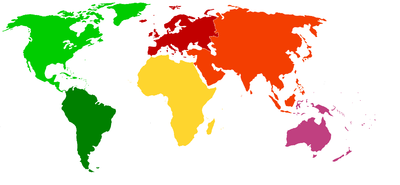
\includegraphics[width=0.6\textwidth]{detaildesign/surface-daily.png}
\caption{Land surface to be acquired in a daily basis}
\label{fig:intr-land-surface}
\end{center}
\end{figure}


\paragraph{Flight Segment}~\\
The satellites are selected according to the current state of the art. However,
some enhancements can be assumed as a way to adjust the analysis to the short
term future.


\subparagraph{Satellite performances}~\\
As a first iteration for the system, small platforms of less of $500~kg$ are
supposed according to the size and payload bay characteristics of representative
platforms in this category. This study is based on the bus platforms currently
offered by Surrey Satellite Technology Ltd, Satrec Initiative and Sierra Nevada Corporation.

In order to reduce the amount of satellites orbiting the Earth, a design with
two payloads was assumed. Thus, the swath (the width of the field of view of each satellite in the surface of the Earth) can be duplicated without decreasing the resolution.

The satellites shall be pointing to nadir, acquiring images without maneuvering
because of the acquisition plan for covering the Earth daily. Simultaneously,
when a satellite gets into the field of view of a Ground Station, the download
of the acquired images starts and at the same time the satellite continues
recording the surface of the Earth.

The main specifications of the satellites in the constellation are shown in Table~\ref{table:intro-satellite-performances}. The values of each parameter were selected according to the state of the art and the desired quality of the images in the mission.

\begin{table}[hp]
  \centering
  {\small
  


\begin{tabular}{p{.2\textwidth}p{.2\textwidth}}
  \tabheadformat
  \tabhead{Specification}   &
  \tabhead{Value}\\
\hline
\textit{GSD}         & $6.7~m$ \\
\hline
\textit{Swath}         & $160~km$ \\
\hline
\textit{Number of bands}         & $5$ \\
\hline
\textit{Digitalization}         & $12~bits$ \\
\hline
\textit{Download Data Rate}         & $160~Mbps$ \\
\hline
\textit{Compression Rate}         &  $2:1$\\
\hline

\end{tabular}


% Local variables:
%   coding: utf-8
%   ispell-local-dictionary: "castellano8"
%   TeX-master: "main.tex"
% End:

  }
  \caption{Main performance parameters of the satellites}
  \label{table:intro-satellite-performances}
\end{table}


\subparagraph{Orbit definition}~\\
The use of \emph{sun-synchronous} orbits in \ac{EO} satellite missions is common. These orbits guarantee that the lighting conditions of the imaged places are the same during the mission, which is a very desirable characteristic.

\ac{LTAN} is also a desired condition of the orbit very related to the lighting
and weather conditions of those places that the satellite overflies (\ac{LTAN}
is selected according to the desired local time of the overflown places and the
cloud formation during the day). The use of \emph{LTAN 10:30h} is commmon for
Earth Observation because at that time the best conditions of cloudiness,
reflectivity and luminosity are given.

Other of the main parameters of an orbit is the altitude. Altitude has effects
in the resolution and the swath of the satellites, which has impact in the
number of satellites required to achieve the coverage objective. According to
the value of those parameters in the payloads included in the satellites, the
reference altitude for the system was found to be $646~km$. \ac{SSO}
condition implies a relation between the altitude and the inclination of the
orbit of $97.97~º$ in this case.

\subparagraph{Number of satellites in the constellation}~\\
The number of satellites is calculated by using the altitude ($646~km$), the
inclination ($97.97~º$) and the swath ($160~km$). As a result, 17 satellites are
required to carry out this mission. In Figure~\ref{fig:intr-constellation-global} the whole constellation is
shown.

\begin{figure}[!h]
\begin{center}
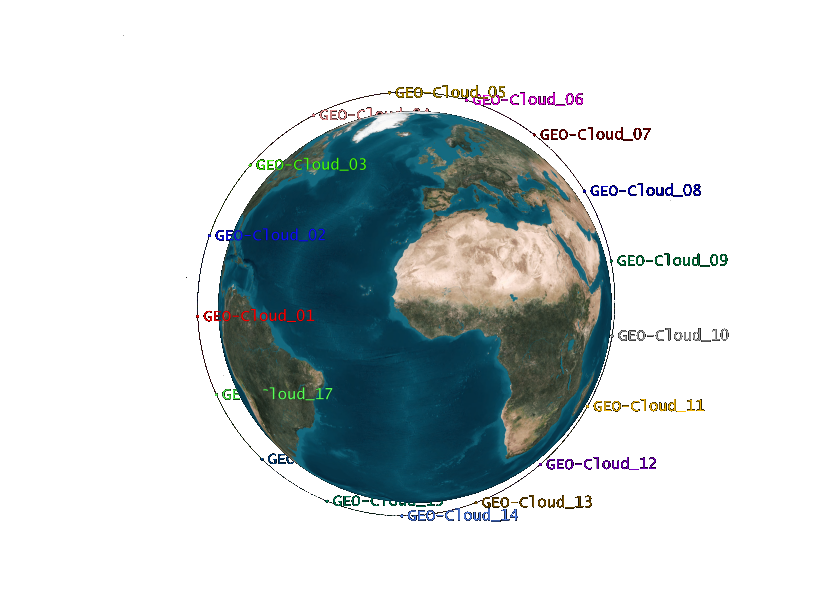
\includegraphics[width=0.75\textwidth]{detaildesign/constellation-global.png}
\caption{Constellation of 17 satellites in a SSO at $646~km$}
\label{fig:intr-constellation-global}
\end{center}
\end{figure}

\paragraph{Ground Stations design}~\\
When the satellite acquires the data, it has to be downloaded to the Ground
Stations. Due to the huge
quantity of data and the limitations to download data rate sets, several
stations distributed over the surface of the Earth are required. They will allow
the satellites to communicate with them and to download the
images. Figure~\ref{fig:intr-footprints} shows how the Ground Stations and their
footprints (area in which the satellites can communicate with the Ground
Station) are distributed.


\begin{figure}[!h]
\begin{center}
\includegraphics[width=0.85\textwidth]{detaildesign/footprints.png}
\caption{Footprints of the selected Ground Stations}
\label{fig:intr-footprints}
\end{center}
\end{figure}

\subsection{Generated Data Volume}

Specifically, $135,698,500~km^2$ of ground surface are daily acquired. With the
following expression can be estimated the data volume generated:

\begin{equation}
Acquired~Data~Volume= \frac{Acquired~Surface}{GSD^2}~*~Nº bands~*~Digitalization
\end{equation}

Before downloading the images they are compressed. The ancillary data is
included in the process (auxiliary information useful for the geolocation of the
images, satellite status and communication protocol among others). In this case, the ancillary data is estimated to be
12\% of the acquired data (based on Deimos 2 satellite measurements), which is
added and then compressed. With the values depicted in
Table~\ref{table:intro-satellite-performances}, the ancillary and the daily ground
surface adquired, the data on ground can be estimated. As a result, including
ancillary data before compression, $11.55~TBytes$  shall be daily downloaded.



\section{Satellite System Development}
\label{sec:spaceSystemSimulator}

This section presents the \sss that emulates the real behaviour of a satellite constellation of 17 satellites that download images to a network of 12 ground stations connected with the \bonfire cloud. The simulator is implemented in \vw.

The \sss is constituted of three components:
\begin{itemize}
\item \satss: it simulates the dynamics and communications of the constellation of 17 Earth observation satellites.
\item \gsss: it simulates the dynamics and communications of the network of 12 ground stations distributed around the World.
\item \emph{Distributed Database:} it contains all the required information and parameters to initialize the simulators and make them run in every specific simulator.
While the \satss and the \gsss are implemented in \vw, the distributed database
is computed in the \bonfire cloud.
\end{itemize}

To adapt the \sss to the Fed4FIRE testbeds, some located scenarios were designed in order to reduce the amount of data to process, store and distribute during the simulations. Thus the simulation is shortened to a specific time required to acquire and download certain areas of interest \emph{(AOI)}.

The detailed design of the \sss and its implementation in \vw are next presented.

\subsection{Image Acquisition}
\label{sec:image-acquisition}

The first step is to implement the acquisition of images by the satellites of
the six predefined scenarios (for an extended description on the scenarios see
Anexo~\ref{anex:scenarios}) with the satellite
constellation:
%\begin{enumerate}[label=\bfseries Scenario \arabic*:]

\begin{enumerate}
\item Emergencies – Lorca Earthquake (Spain)
\item  Infrastructure monitoring. Affection in railway infrastructures by sand movement in desert areas (Spain)
\item Land Management – South West of England
\item Precision Agriculture – Argentina
\item Basemaps – Worldwide
\end{enumerate}

In each scenario, an Area of Interest \emph{(AOI)} is defined to be acquired
during the simulation. The in orbit satellites are nadir pointing in order to acquire images of the sub satellite point over the Earth surface as shown in Figure \ref{fig:sss-example-strip}.
\begin{figure}[!h]
\begin{center}
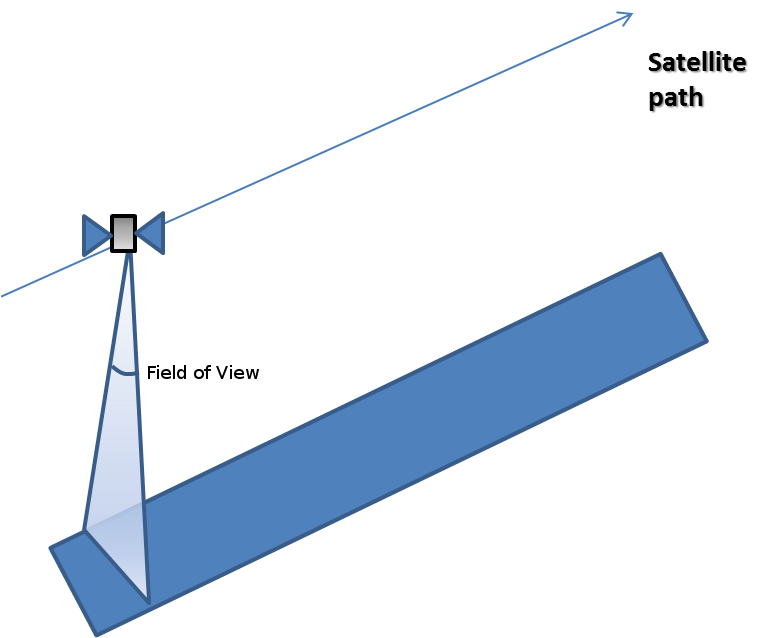
\includegraphics[width=0.6\textwidth]{spaceSystemSimulator/strip-imaging.png}
\caption{Example of strip imaging}
\label{fig:sss-example-strip}
  \end{center}
\end{figure}

In the next subsection the assumptions to simulate the system as realistically
as possible are described for the scenarios. Note that the \emph{AOI} of the scenario 5 is the whole land mass on Earth. This involves that because of the huge amount of data that has to be recorded, specific assumptions to the scenario 5 was made according to the Fed4FIRE testbeds’ limitations.

\subsubsection{Assumptions in satellite image acquisition}
\label{subsubsec:assumptions}

The \emph{AOI} in each scenario can be acquired by one or more satellites depending on
the size of the \emph{AOI} relatively to the scene size (note that the GEO-Cloud
satellites have a swath of $160~km$, thus we divide the acquisition into scenes of
$160~km$ x $160~km$).
In each scenario we call \emph{main satellites} to the satellites with the task
of acquiring the \emph{AOI} (note that all satellites are \emph{main satellites} in the
model for the scenarios 5 and 6).

Along the duration of the scenario other satellites acquire images of the areas
of the Earth surface they are passing over. Those images are not in the area of
interest.

During the experiments in \bonfire, they will be processed but not stored into the system, since the focus of the mission in every scenario has to be in the defined area of interest. Those non \emph{AOI} images allow us to emulate a real system, since we take into account all the possible inputs to the system (note that in the scenarios 5 and 6 all the images created are \emph{AOI}).


\begin{figure}[!h]
\begin{center}
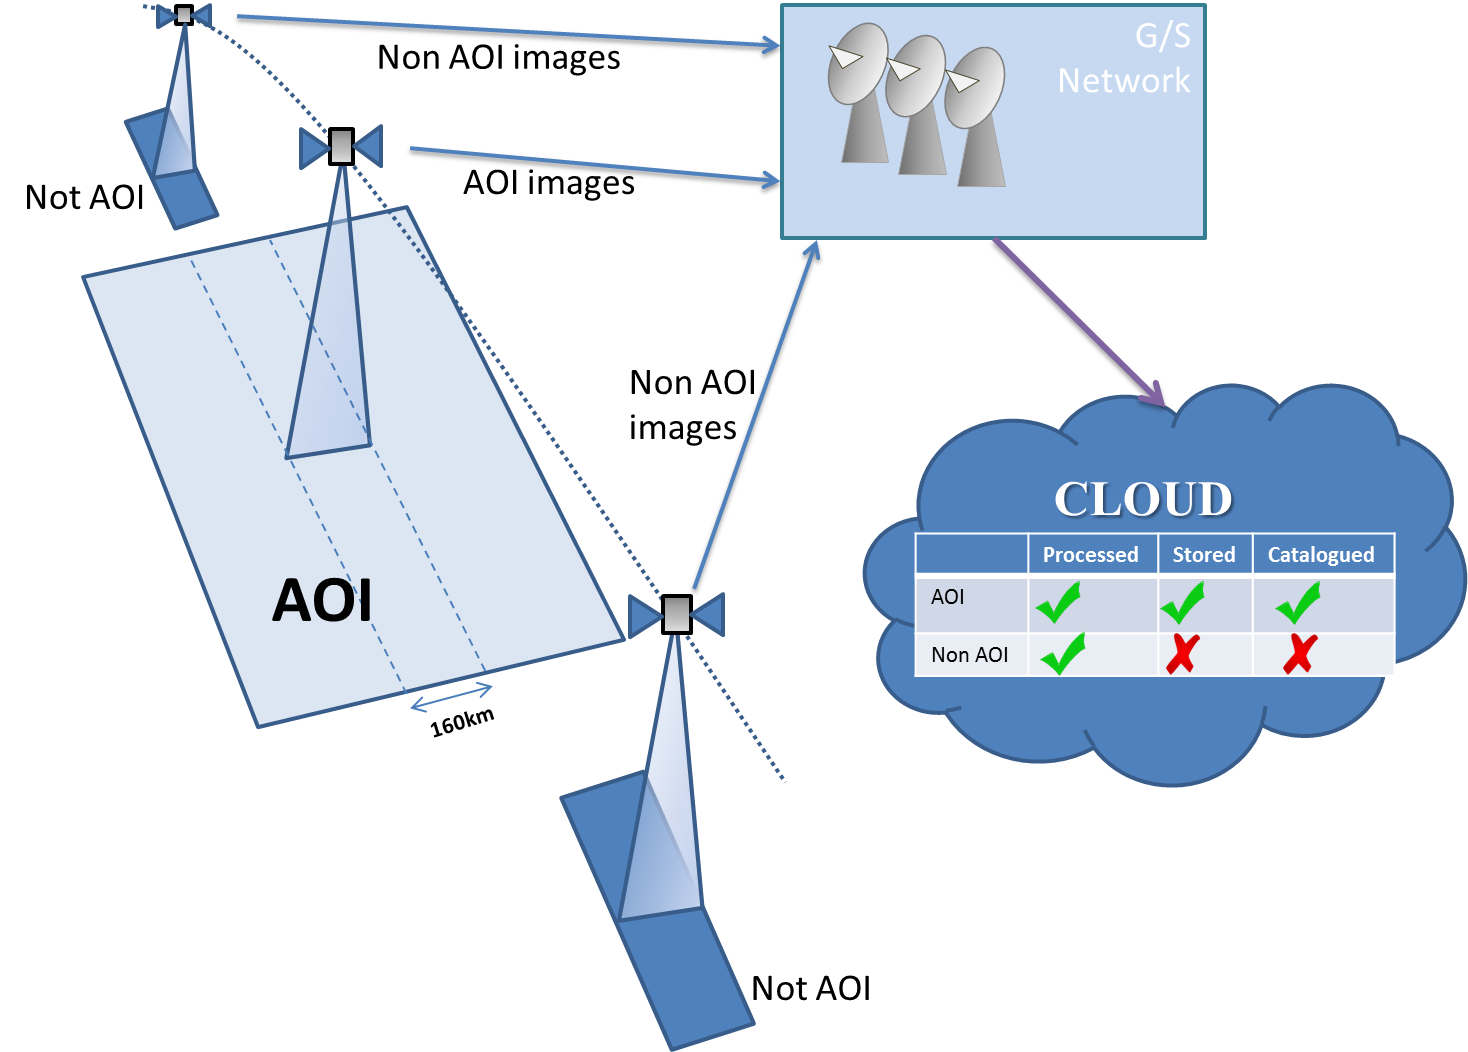
\includegraphics[width=0.8\textwidth]{spaceSystemSimulator/images-adquisition-diagram.png}
\caption{Diagram of images adquisition}
\label{fig:sss-acquisition-diagram}
\end{center}
\end{figure}

Thus, those non \emph{AOI} images, during the simulation will be acquired,
downloaded to the ground stations, transferred to the cloud and processed, but
not stored, neither catalogued. In addition, it has to be taken into account
that the main satellites can also acquire some images out of the \emph{AOI}
during the duration of each scenario. Those acquired images are also considered
non \emph{AOI} images.

In every scenario the time is set to 0 when the simulation starts in the Fed4FIRE environment.

These assumptions are summarized as follows:
\begin{enumerate}
\item Only the scenes acquired by a satellite that include the \emph{AOI} are considered to carry out the complete simulation.
\item Images taken by the satellites that are out of the \emph{AOI} are processed but
  not stored into the system to adjust the experiment execution to the resources
  provided by \bonfire.
\end{enumerate}

\subsubsection{Types of acquisition of the AOI by a single satellite}
\label{subsubsec:types-acquisition}

Depending on the relative sizes of both the \emph{AOI} and the scenes, three different
situations can occur when a single satellite is acquiring images (see Figure~\ref{fig:sss-types-aoi-acquisitions}):
\begin{itemize}
\item Simple acquisition: the \emph{AOI} (at least the part to be imaged by the
  satellite) fits into just one scene.

% \begin{figure}[!h]
% \begin{center}
% 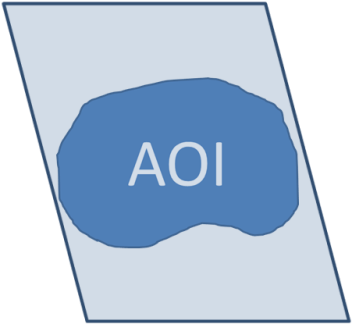
\includegraphics[width=0.3\textwidth]{spaceSystemSimulator/simple-acquisition.png}
% \caption{Simple acquisition}
% \label{fig:sss-simple-acquisition}
% \end{center}
% \end{figure}
\item Multiple consecutive acquisitions: the \emph{AOI} to be acquired by a satellite
fits in a strip with several scenes.
% \begin{figure}[!h]
% \begin{center}
% 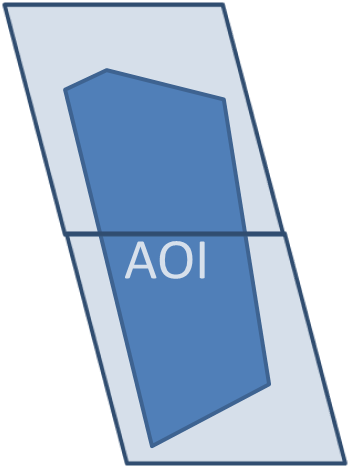
\includegraphics[width=0.3\textwidth]{spaceSystemSimulator/multiple-consecutive-acquisitions.png}
% \caption{Multiple consecutive acquisitions}
% \label{fig:sss-multiple-acquisition-diagram}
% \end{center}
% \end{figure}

\item Multiple non-consecutive acquisitions: the \emph{AOI} to be acquired by a
  satellite fits in a strip but there are some scenes between the acquisitions
  that have to be acquired in order to complete the general mission (world map
  daily) but it is not necessary for the scenario.
\end{itemize}

% \begin{figure}[!h]
% \begin{center}
% 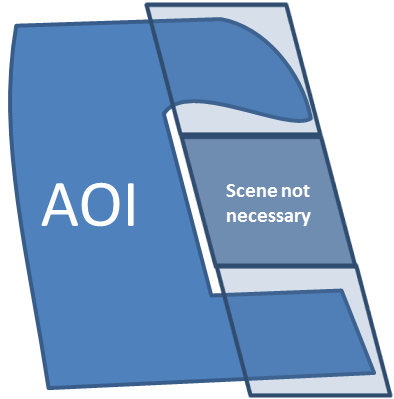
\includegraphics[width=0.3\textwidth]{spaceSystemSimulator/non-consecutive-acquisitions.png}
% \caption{Multiple non-consecutive acquisitions}
% \label{fig:sss-non-consecutive-acquisition}
% \end{center}
% \end{figure}
\begin{figure*}
\begin{center}
  \subfloat[Simple acquisition]{
    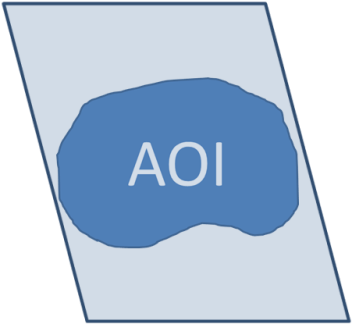
\includegraphics[width=0.25\textwidth]{spaceSystemSimulator/simple-acquisition.png}
    \label{fig:sss-simple-acquisition}
  }
 \hspace{0.01\textwidth}
 \subfloat[Multiple consecutive acquisitions]{
    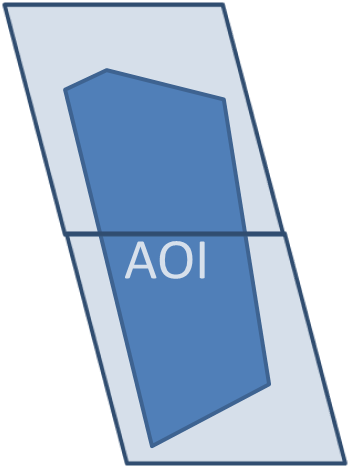
\includegraphics[width=0.25\textwidth]{spaceSystemSimulator/multiple-consecutive-acquisitions.png}
    \label{fig:sss-multiple-consecutive-acquisition}
  }
\hspace{0.01\textwidth}
 \subfloat[Multiple non-consecutive acquisitions]{
    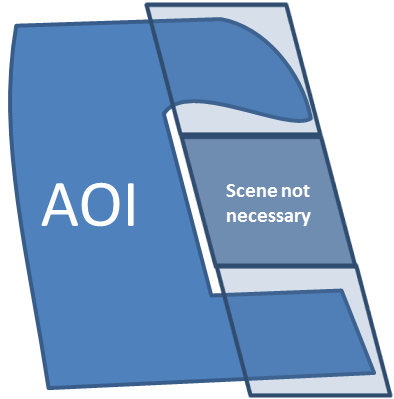
\includegraphics[width=0.25\textwidth]{spaceSystemSimulator/non-consecutive-acquisitions.png}
    \label{fig:sss-non-consecutive-acquisition}
  }
\caption{Different types of the AOI acquisitions}
\label{fig:sss-types-aoi-acquisitions}
\end{center}
\end{figure*}



\subsubsection{Parameters required for the simulation of the scenarios}
\label{subsubsec:parameters-required}
For each scenario, the following parameters and assumptions are considered:
\begin{enumerate}
\item \emph{S: Scenario number.} It indicates the scenario that is being simulated (from 1 to 6).
\item \emph{Main satellites:} The main satellites are those that acquire images of the AOI in each scenario. Notice that all the satellites are numbered from 1 to 17.
\item \emph{ADR:} Acquisition Data Rate. Rate at which the images are acquired
  by the satellite.

\begin{equation} \label{eq:ADR}
ADR=1395~Mbps
\end{equation}

\item \emph{CR:} Compression Rate. Rate at which the images are compressed in
  the satellite for their download.
\begin{equation}\label{eq:CR}
CR=14.1
\end{equation}
\item \emph{$Bandwidth_{sat}$:} Download rate between the satellites and the
  ground stations.
\begin{equation}\label{eq:Bandwidth}
Bandwidth_{sat}=160~Mbps
\end{equation}

The previous bandwidth is used as follows:
\begin{itemize}
\item The satellite is downloading images in memory and at the same time is
  acquiring images and downloading them:
\begin{equation}\label{eq:totalBandwidth}
Bandwidth_{sat}=Bandwidth_{(sim\_acq)}+Bandwidth_{mem}
\end{equation}

where $Bandwidth_{(sim\_acq)}$ is the bandwidth used for downloading images that
are being acquiring at the same time and $Bandwidth_{mem}$ is the bandwidth used
to download images in the satellite memory. $Bandwidth_{(sim\_acq)}$ can be
obtained as follows:
\begin{equation}\label{eq:bandwidth-sim}
  Bandwidth_{(sim\_acq)}=\frac{ADR}{CR}=98.9~Mbps
\end{equation}

where \emph{ADR} is the Acquisition Data Rate (Mbps) and \emph{CR} the data
compression rate. And $Bandwidth_{mem}$ can be obtained as follows:
\begin{equation}\label{eq:bandwidth-mem}
  Bandwidth_{mem}=Bandwidth_{sat}-Bandwidth_{(sim\_acq)}=61.1~Mbps
\end{equation}
\end{itemize}

\item \emph{$T_0$:} Start time. It is the start time of the scenario. The scenario starts when the first main satellite begins the acquisition of the first portion of \emph{AOI}.
\item \emph{$T_f$:} End time. It is the time when the last main satellite finishes the downloading of the \emph{AOI} taken images.
\item \emph{$[T_{AOI}]_{0i}$:} Time a main satellite starts acquiring the \emph{AOI}. $i$ stands for the number of the main satellite.
\item \emph{$[T_{AOI}]_{fi}$:} This is the time a main satellite finishes acquiring a piece of \emph{AOI}.
\item \emph{$[\Delta T_{AOI}]_i$:} This is the difference
  $[T_{AOI}]_{fi}-[T_{AOI}]_{0i}$. Note: Some satellites (all of them in the
  model for scenario 5) can require more than one orbit to acquire the
  corresponding \emph{AOI}, and then these satellites will have a different
  $[\Delta T_{AOI}]_i$ in each acquisition of \emph{AOI}. $[\Delta T_{AOI}]_i$
  is a multiple of  $T_{scene}=23.4~s$, which is the needed time to acquire one
  scene of $160~km$x $160~km$, considering that satellite velocity on ground is
  $v_{Gsat}=6.84~km/s$:
\begin{equation}\label{eq:Tscene}
	T_{scene}=L_{scene}/v_{Gsat}
\end{equation}

$[\Delta T_{AOI}]_i$  can be calculated as follows:
\begin{equation}\label{eq:deltataoi}
[\Delta T_{AOI}]_i=n L_{scene}/v_{Gsat} =nT_{scene}=[T_{AOI}]_{fi}-[T_{AOI}]_{0i}
\end{equation}

where $n$ is the number of scenes, $L_{scene}$  is the length of the scene (in
this case $160~km$), and $v_{Gsat}$ the velocity of the satellite on ground (in this case $6.84~km/s$).
\item \emph{$[T_{GS}]_{0ij}$:} Time a main satellite $i$ enters into the visibility cone of a \emph{Ground Station} $j$.
\item \emph{$[T_{GS}]_{fij}$:} Time a main satellite $i$ leaves the visibility cone of a Ground Station  $j$.
\item \emph{$[\Delta T_{GS}]_{ij}$:} This is the difference $[T_{GS}]_{fij}-[T_{GS}]_{0ij}.$
\item \emph{$T_{start}$:} This is the start time of the simulation. We chose to be $5$ seconds in order to synchronize all the satellites.

\end{enumerate}

As an example, the Table~\ref{table:sss-acquisitions-scenario2} shows the data was obtained from ``Scenario 2: Infrastructure monitoring affection in railway infrastructures by sand movement in desert areas'':

\begin{table}[h]
  \centering
  {\small
  


\begin{tabular}{c c c c c c c}\hline
\tabheadformat
\tabhead{Scenario} & \tabhead{Start Time} &
\tabhead{End Time} & \tabhead{Main} & \tabhead{Start} &
\tabhead{End} &\tabhead{Number of}\\
\tabheadformat
 & $T_0$&$T_f$ &\tabhead{Satellite} & \tabhead{Acquisition}&\tabhead{Acquisition} &\tabhead{\emph{AOI} scenes}\\
 \tabheadformat
 & & & & $[T_{AOI}]_{0i}$&$[T_{AOI}]_{fi}$ & \\\hline
\multirow{3}{*}{2} & \multirow{3}{*}{54060} & \multirow{3}{*}{54753.4}&4 & 54060&54083.4&\multirow{3}{*}{1} \\\cline{4-6}
                   &        &         & 3 & 54390&54413.4 \\\cline{4-6}
                   &        &         & 2 & 54730&54753.4  \\\hline      
\end{tabular}

  }
  \caption{Example of data of image acquisition for Scenario 2}
  \label{table:sss-acquisitions-scenario2}
\end{table}


\subsection{Image Downloading}
\label{subsec:image-downloading}

The acquired images by the satellites shall be downloaded to the emulated ground
stations through the antennas network designed (see Section~\ref{subsec:system-design}). All the scenarios finish at $T_f$, when the last
main satellite completely downloads the last acquired portion of the
\emph{AOI}. During the simulation, the rest of the satellites not overflying the
\emph{AOI} would be imaging other places; these images will also be downloaded
and processed in parallel to the \emph{AOI} images to simulate a realistic case,
but as previously explained those images will not be stored nor catalogued.

Because of the limitations in the testbeds (limited storage and compute
resources in \bonfire cloud and multiplexed channel over virtual networks in
\vw) it is necessary to scale the data involved in these simulations from the
original design of the GEO-Cloud experiment. It has been decided to change the
designed compression rate from lossless compression $2:1$ to a rate compression
$14:1$. With this change, the data volume has been reduced and the size of every
$160km$ x $160km$ scene after compression is now $288~MB$ instead of the almost
$2~GB$ size of the original images.

In order to download the data, the satellites have to be inside the visibility
cone of a ground station. During these accesses, the satellites download images
at a rate of $160~Mbps$. Part of these images are in memory before entering the
visibility cone and others are being acquired simultaneously during the
downloading task (see section \ref{subsubsec:parameters-required} for a wider explanation of the download parameters and Figure \ref{fig:sss-multiplexed-downloading}).

\begin{figure}[!h]
\begin{center}
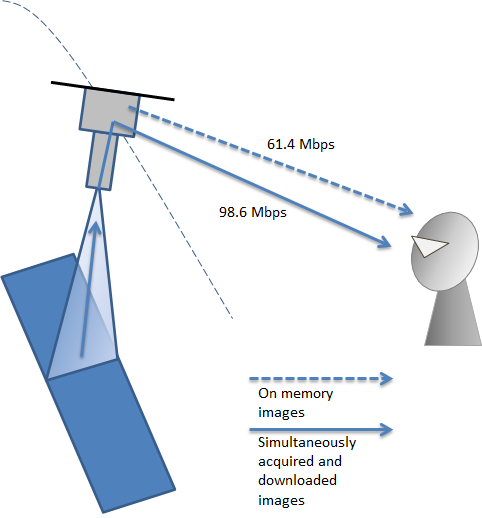
\includegraphics[width=0.5\textwidth]{spaceSystemSimulator/multiplexed-downloading.png}
\caption{Multiplexed images downloading}
\label{fig:sss-multiplexed-downloading}
\end{center}
\end{figure}



It is possible that the duration of the accesses and the time to download an image are not multiples of $T_{scene}=23.4~s$. In this case, an image would be partially downloaded at the end of the access but it would be supposed that this image is completely downloaded in the following access in other ground station.

For the memory management, a \emph{LIFO} (last in, first out) procedure is
applied. This implies that the latest acquired images will be downloaded as soon
as possible. This imposes that when a satellite is inside the visibility cone of
a ground station both the images latest acquired and the images that are being
acquired of the \emph{AOI} will be simultaneously downloaded by multiplexing
them. Note that because of differences between the rate of acquisition and
downloading, and also because of the compression process, the downloading of
images that are being simultaneously acquired do not occupy all the bandwidth of
$160~Mbps$; the portion not occupied is used to download on board storage also
with a \emph{LIFO} process (See section \ref{subsubsec:parameters-required} numbers 3 to 5).


As an example, the data of the accesses for the Scenario 2 are included in Table~\ref{table:sss-accesses-scenario2}.


\begin{table}[h]
  \centering
  {\small
  
\begin{tabular}{p{.2\textwidth}p{.2\textwidth}c c c}\hline
\tabheadformat
\tabhead{Sat. Ident. Number} & \tabhead{Ground Station} &
\tabhead{Access Start Time} & \tabhead{Access Stop Time}
&\tabhead{Duration of the passes}\\
\tabheadformat
 & &$(s)$ &$(s)$ &$(s)$ \\\hline
        1 & Krugersdorp  & 54184.2 &54516 &331.8\\\hline
        2 & Dubai        & 54184.2 &54516 &331.8\\\hline
        2 & Krugersdorp  & 54549.4&54753.4 &204\\\hline
        3 & Dubai        & 54060 &54753.4&204\\\hline
        4 & Dubai        &54060&54337.5&277.5\\\hline              
        4 & Svalvard     &54660&54753.4&93.4\\\hline
        5 & Svalvard     &54316.3&54753.4&437.1\\\hline
        6 & Prince Albert&54708.1&54753.4&45.3\\\hline
        6 & Svalvard     &54060&54639.4&579.4\\\hline
        7 & Prince Albert&54362&54753.4&391.4\\\hline
        7 & Svalvard     &54060&54296.7&236.7\\\hline
        8 & Prince Albert&54060&54577.9&517.9\\\hline
        9 & Prince Albert&54060&54246.8&186.8\\\hline
        15 & Troll       &54419&54670.3&251.3\\\hline
        16 & Troll       &54085.6&54303.4&217.8\\\hline
        17 &Krugersdorp  &54495.4&54753.4&258\\\hline              
\end{tabular}

  }
  \caption{Example of data of accesses for Scenario 2}
  \label{table:sss-accesses-scenario2}
\end{table}


Next, a summary of the assumptions made for the image downloading from the
satellites to the ground stations are described:
\begin{enumerate}
\item Time to process the images on board before downloading is considered to be instantaneous. Then, the simultaneous acquisition and download of the \emph{AOI} inside the visibility cone is done without latency.
\item The ground stations network was designed to guarantee the download of a complete world map in a daily basis. With this assumption into account, the management of the memory on board of each satellite does not require an additional design. This involves that we do not know in which ground station all the areas acquired out of a visibility cone are downloaded.
\item Because of the small gap between the satellites, which are in the same orbit, more than one antenna in each ground station is required to be available. This provides the possibility of having simultaneous contacts with all the satellites inside the visibility cone.
\end{enumerate}

\subsection{Getting the satellite data}
\label{subsec:getting-satellite-data}

The steps to obtain and simulate the realistic behaviour of the satellites are
next described.


\subsubsection{Extraction of the real behaviour of the satellite constellation
  in the scenarios}
\label{subsubsec:extraction}

The first point is to obtain the realistic behaviour of the constellation of satellites designed in section~\ref{subsec:system-design}.  For that purpose, the constellation of satellites and the ground stations were implemented in the \emph{$Systems Tool Kit^{\textregistered}$} (\acs{STK}) software.

The next steps were followed to obtain the values of the parameters required for the simulations of the defined scenarios:
\begin{itemize}
\item Commonly for all the scenarios:
\begin{enumerate}
\item Implementation of the satellite constellation.
\item Implementation of the ground station network.
\item Calculation of the access time for each satellite communicating with each
  ground station during 24 hours.
\newcounter{enumTemp}
\setcounter{enumTemp}{\theenumi}
\end{enumerate}
\item For each different scenario:
\begin{enumerate}
\setcounter{enumi}{\theenumTemp}
\item Identification of the main satellites.
\item Extraction of the times each satellite is acquiring the AOI: $[T_{AOI}]_{0i}$ and $[T_{AOI}]_{fi}$.
\item Calculation of the number of scenes acquired: $n$.
\item Extraction of the access duration of each satellite with the ground stations it communicates within the scenario duration: $[T_{GS}]_{0ij}$ and $[T_{GS}]_{fij}$.
\item Start time of the scenario: $T_0$.
\item End time of the scenario: $T_f$.
\end{enumerate}
\end{itemize}

\subsubsection{Exportation of data to the simulator}

Once obtained the previous data, it is exported to different \ac{CSV} format files:

\begin{itemize}
\item 	The \emph{Scenario\_<NUM>\_<SCENE>.csv} files: it contains the information
  of the $[T_{GS}]_{0ij}$ and $[T_{GS}]_{fij}$ for each scenario. \emph{<NUM>} indicates
  the number of the scenario and \emph{<SCENE>} the name of the scenario. In the
  GEO-Cloud experiment we simulate 6 scenarios. The previous parameters are
  defined in the following table:


For example, the format of the resulting \emph{Scenario\_1\_
Emergencies\_Lorca\_Earthquake.csv} file with the $[T_{GS}]_{0ij}$ and $[T_{GS}]_{fij}$
information for the Lorca scenario, looks like the code extract shown in Listing
\ref{code:sss-info-scenario}.
\begin{listing}[
  float=h!,
  caption  = {Extract of the \emph{Scenario\_1\_Emergencies\_Lorca\_Earthquake.csv}
    of the Lorca scenario},
  label    = code:sss-info-scenario,
style=customc]
"GEO-Cloud_005-To-Troll - Access","Start Time (EpSec)","Start Time (UTCG)","Stop Time (EpSec)","Stop Time (UTCG)","Duration (sec)"
1,63638.000,11 Aug 2014 10:10:38.000,63661.400,11 Aug 2014 10:11:01.400,23.400

"GEO-Cloud_006-To-Troll - Access","Start Time (EpSec)","Start Time (UTCG)","Stop Time (EpSec)","Stop Time (UTCG)","Duration (sec)"
7,63638.000,11 Aug 2014 10:10:38.000,63661.400,11 Aug 2014 10:11:01

\end{listing}
In the code, a heading is separated into columns. It is divided as the
table~\ref{table:sss-headings-scenario2} shows.

\item 	The \emph{All\_Scenarios.csv} file: it contains the information of the $[T_{AOI}]_{0i}$ and $[T_{AOI}]_{fi}$ for all the scenarios.
A piece of the \emph{All\_Scenarios.csv} file that contains the $[T_{AOI}]_{0i}$
and $[T_{AOI}]_{fi}$ of all the scenarios is shown in Listing~\ref{code:sss-all-scenarios}.  It also contains  $T_0$ ,$T_f$ and the number $n$ of \emph{AOI} obtained images.


\begin{listing}[
  float=h!,
  caption  = {Extract of the \emph{All\_Scenarios.csv} code of the Lorca scenario},
  label    = code:sss-all-scenarios,
style=customc]
Scenario,Start Sce,End Sce,Sat,Start sat,End Sat,Images
1,63638,63661.4,11,63638,63661.4,1
,,,,,,
2,54060,54753.4,4,54060,54083.4,1
,,,3,54390,54413.4,1
,,,2,54730,54753.4,1
,,,,,,
3,62480,63865.4,15,62480,62503.4,1
,,,14,62821,62844.4,1
,,,13,63161,63184.4,1
,,,12,63501,63524.4,1
,,,11,63842,63865.4,1
\end{listing}

This file was manually computed. The required fields to describe the behaviour
of the satellites acquiring the \emph{AOI} are the depicted in Table~\ref{table:sss-all-scenarios}.

%\begin{multicols}{2}
%\begin{center}
\begin{table}[h]
  \centering
  {\small
  


\begin{tabular}{p{.2\textwidth}p{.2\textwidth}}
  \tabheadformat
  \tabhead{Column Title}   &
  \tabhead{Function}\\
\hline
\textit{GEO-Cloud\_sat-To-station}         & Represents the access of a satellite to the specific ground station. sat represents the satellite number and station the ground station name. \\
\hline
\textit{Start Time (EpSec)}         & Means $[T_{GS}]_{0ij}$. \\
\hline
\textit{Start Time (UTCG)}         & Means  $[T_{GS}]_{0ij}$ in UTCG format \\
\hline
\textit{Stop Time (EpSec)}         & Means $[T_{GS}]_{fij}$ \\
\hline
\textit{Stop Time (UTCG)}         & Means $[T_{GS}]_{fij}$ in UTCG format. \\
\hline
\textit{Duration (sec)}         & Means $[\Delta T_{GS}]_{ij}$. \\
\hline
\end{tabular}


% Local variables:
%   coding: utf-8
%   ispell-local-dictionary: "castellano8"
%   TeX-master: "main.tex"
% End:

  }
  \caption{Columns headings \emph{Scenario\_<NUM>\_<SCENE>.csv} files}
  \label{table:sss-headings-scenario2}
\end{table}
%\end{center}

%\columnbreak
%\begin{center}
\begin{table}[h]
  \centering
  {\small
  


\begin{tabular}{p{.2\textwidth}p{.2\textwidth}}
  \tabheadformat
  \tabhead{Column Title}   &
  \tabhead{Function}\\
\hline
\textit{Scenario}         & Scenario number. Indicates the scenario executed \\
\hline
\textit{Start Sce}         & Indicates the start of the scenario. It is $T_0$  \\
\hline
\textit{End Scen}         &Indicates when the scenario finishes. It is $T_f$ \\
\hline
\textit{Sat}         & Indicates the number of the \emph{main satellite}.\\
\hline
\textit{Star Sat}         & The time when the satellite starts acquiring the \emph{AOI}. It is $[T_{AOI}]_{0i}$. \\
\hline
\textit{End Sat}         & The time when the satellite finishes acquiring the \emph{AOI}. It is $[T_{AOI}]_{fi}$ \\
\hline
\textit{Images}         & This is the number of \emph{AOI} images. It is $n$.\\
\hline
\end{tabular}


% Local variables:
%   coding: utf-8
%   ispell-local-dictionary: "castellano8"
%   TeX-master: "main.tex"
% End:

  }
  \caption{Columns headings of the \emph{All\_Scenarios.csv} file}
  \label{table:sss-all-scenarios}
\end{table}
%\end{center}
%\end{multicols}
\end{itemize}


\subsubsection{Processing of the Scenario\_<NUM>\_<SCENE>.csv and
 All\_Scenarios.csv}
\label{subsubsec:processing-files}

A script is designed and developed to get and merge the data from the \emph{Scenario\_<NUM>\_<SCENE>.csv} and the \emph{All\_Scenarios.csv} files, and to store the information in the database:  \emph{setDatabase.py}. It was developed in Python 2.7 but it is also compatible with all Python versions.

This has to be done because as previously explained
\emph{Scenario\_<NUM>\_<SCENE>.csv} contains the $[T_{GS}]_{0ij}$ and $[T_{GS}]_{fij}$
parameters of each single scenario and \emph{All\_Scenarios.csv} the
$[T_{AOI}]_{0i}$ and $[T_{AOI}]_{fi}$ of all the scenarios. Thus the script matches the
$[T_{GS}]_{0ij}$ and $[T_{GS}]_{fij}$ of one scenario with the $[T_{AOI}]_{0i}$ and $[T_{AOI}]_{fi}$ of such a scenario.

To execute \emph{setDatabase.py} the arguments depicted in Table~\ref{table:sss-arguments-setdatabase} are required.
\begin{table}[h]
  \centering
  {\small
  


\begin{tabular}{p{.2\textwidth}p{.2\textwidth}}
  \tabheadformat
  \tabhead{Argument Position}   &
  \tabhead{Meaning}\\
\hline
\textit{1}         & IP direction of the host which contains the MySQL database\\
\hline
\textit{2}         & The relative path or absolute path of the file that contains the information of all scenarios (see Listing \ref{code:sss-all-scenarios})
  \\
\hline
\textit{3\ldots}         &The \emph{Scenario\_<NUM>\_<SCENE>.csv} files that contain the events occurred in a particular scenario. At least one file must be introduced, otherwise an execution error is produced. \\\hline
\end{tabular}


% Local variables:
%   coding: utf-8
%   ispell-local-dictionary: "castellano8"
%   TeX-master: "main.tex"
% End:

  }
  \caption{Arguments of \emph{setDatabase.py}}
  \label{table:sss-arguments-setdatabase}
\end{table}

An example of the execution of the programme is the following:
\begin{itemize}
\item[>] python~setDatabase.py~192.168.0.2~All\_scenarios\_file.csv~Scenario\_1\_Example1.csv~Scenario\_2\_Example2.csv~Scenario\_3\_Example3.csv
\end{itemize}


\subsection{Space System Simulator}

The \sss is constituted by the following modules:
\begin{itemize}
\item The Database
\item The \satss
\item The \gsss
\end{itemize}


To simulate every scenario, on the one hand, the \satss is executed. It is
constituted by 17 \emph{Satellite Simulators} of individual satellites; each one
reproduces the characteristic behaviour of every single satellite in the
constellation.
On the other hand the \gsss is also executed. As in the case of the \satss, the
\gsss is constituted of 12 \emph{Ground Station Simulators} of individual ground
stations reproducing the behaviour of every single ground station of the
designed network.

The diagram in Figure~\ref{fig:sss-architecture} depicts a scheme
representing the \emph{Space System Simulator}.

\begin{figure}[!h]
\begin{center}
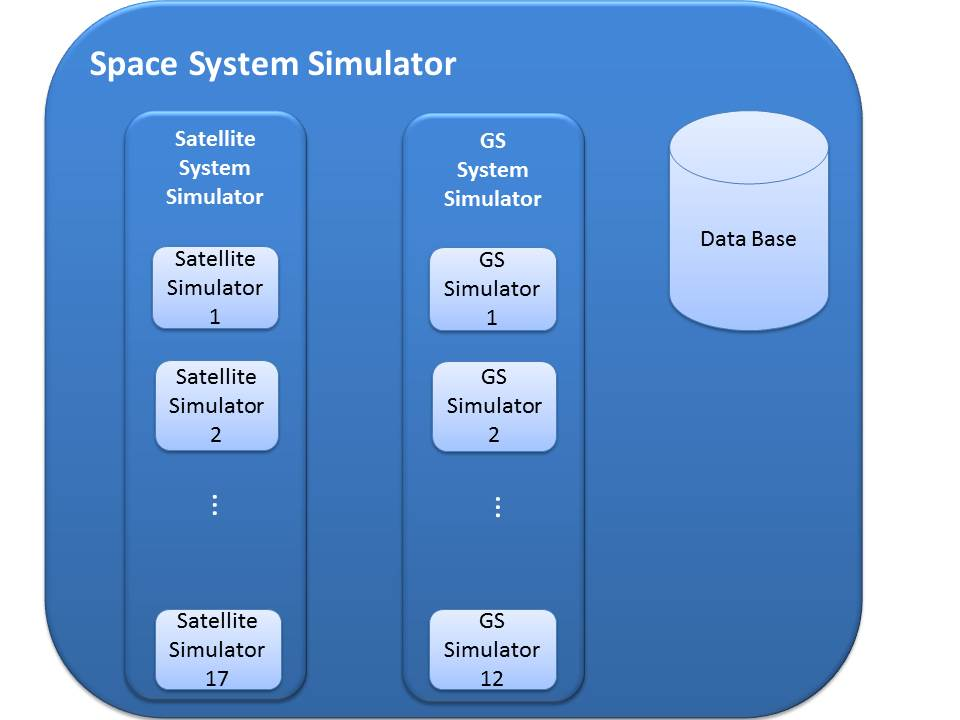
\includegraphics[width=0.8\textwidth]{spaceSystemSimulator/sss-architecture.jpg}
\caption{Space System Simulator's Architecture}
\label{fig:sss-architecture}
\end{center}
\end{figure}

The Space System Simulator sequentially follows the next steps during the
execution:
\begin{itemize}

\item First, \emph{setDatabase.py} is executed. The script fills the database fields with the information of every scenario.
\item Second, the \gsss is executed. The \gsss can execute all the \emph{Ground Station Simulators} or some of them individually to simulate faults in the ground stations as it can occur in reality. Thus, when a satellite needs to download data into a ground station that is offline, it will receive an exception so the downloading of images does not start.
\item Third, the \satss is executed. As in the previous case, the \satss can execute all the \emph{Satellites Simulators} or some of them individually for the same reason.
\item Finally, when the scenario finishes, the simulation is stopped.
\end{itemize}
The \emph{Database}, the \satss and the \gsss are thoroughly described in the
next subsections.

\subsubsection{Database}

A database containing all the required data for the simulations was
implemented. The selected database management system \emph{(DBMS)} is
\emph{MySQL}. It was selected because it is friendly usable, works in multiple
platforms, provides transactional and nontransactional storage engines and the server is a separate program for use in a \emph{client/server} networked environment.

The design of the database architecture is shown in Figure~\ref{fig:sss-database-architecture}.

\begin{figure}[!h]
\begin{center}
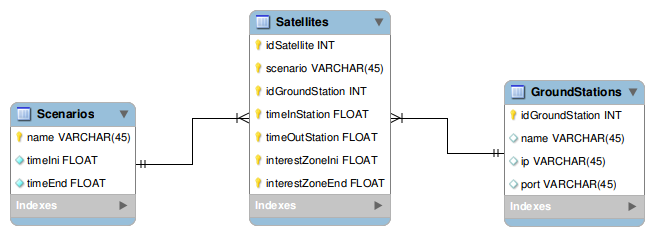
\includegraphics[width=0.85\textwidth]{spaceSystemSimulator/database-architecture.png}
\caption{Database architecture}
\label{fig:sss-database-architecture}
\end{center}
\end{figure}

The database is constituted by three tables: \emph{Scenarios table},
\emph{Satellites table} and \emph{GroundStations table}. The functionalities of the tables are described in
Table~\ref{table:sss-funcionalities-database}.

% \begin{table}[h]
%   \centering
%   {\small
%   


\begin{tabular}{p{.2\textwidth}p{.2\textwidth}p{.2\textwidth}p{.2\textwidth}}
  \tabheadformat
  \tabhead{Table}   & \tabhead{Function}& \tabhead{Columns} &
  \tabhead{Relationship}\\\hline

\textit{Scenarios table}    &  It contains the name of the scenario, the start
time $T_0$ and the end time $T_f$. Its primary key\footnote{The \emph{primary
    key} identifies an object; for example a scenario, a ground station or a
  satellite} (represented with a key symbol in
Figure~\ref{fig:sss-database-architecture}) is the name column.   & name timeIni
timeEnd&None\\
\hline


\textit{GroundStations table} & It contains the ID of the Ground Station and its
name. Its \emph{primary key} is the idGroundStation. &
idSatellite scenario idGroundStation timeInStation timeOutStation
interestZoneIni interestZoneEnd
&None  \\\hline

\textit{Satellites table} &  It contains the ID of the satellites
\emph{idSatellite}, the scenario and the ground station id,
\emph{idGroundStation}, in which the events occur, the time in which the
satellite enters into the visibility cone $[T_{GS}]_{0ij}$,
\emph{timeInStation}, the time when it leaves the visibility cone
$[T_{GS}]_{fij}$, \emph{timeOutStation}, the time when the satellite enters into
the \emph{AIO} $[T_{AOI}]_{0i}$, \emph{interestZoneIni}, and the time when the
satellite leaves the \emph{AOI} $[T_{AOI}]_{fi}$,\emph{interestZoneEnd}. All of
them are primary keys because a satellite can download images of several
\emph{AOIs} in a single ground station.
  & idGroundStation name ip port & This table relates the \emph{Scenarios} table and the \emph{GroundStations} table. This is because the \emph{scenario} and \emph{idGroundStation} columns are foreign keys\footnote{The \emph{foreign key} binds two tables, linked across a field. For example in this case, the column from the \emph{Satellites} table which is named \emph{Scenario} refers to an object that exists in the \emph{Scenarios} table.}. The characteristics of these columns are \emph{On delete cascade} and \emph{On update cascade}. This means that when an object contained in a table (\emph{GroundStation} table or \emph{Scenarios} table) is deleted, it is also automatically deleted the object that refers to it, and if it is updated the object is also automatically updated. \\\hline
\end{tabular}


% Local variables:
%   coding: utf-8
%   ispell-local-dictionary: "castellano8"
%   TeX-master: "main.tex"
% End:

%   }
%   \caption{Funcionalities of the database tables for the simulator}
%   \label{table:sss-funcionalities-database}
% \end{table}
 


\begin{tabular}{p{.2\textwidth}p{.2\textwidth}p{.2\textwidth}p{.2\textwidth}}
  \tabheadformat
  \tabhead{Table}   & \tabhead{Function}& \tabhead{Columns} &
  \tabhead{Relationship}\\\hline

\textit{Scenarios table}    &  It contains the name of the scenario, the start
time $T_0$ and the end time $T_f$. Its primary key\footnote{The \emph{primary
    key} identifies an object; for example a scenario, a ground station or a
  satellite} (represented with a key symbol in
Figure~\ref{fig:sss-database-architecture}) is the name column.   & name timeIni
timeEnd&None\\
\hline


\textit{GroundStations table} & It contains the ID of the Ground Station and its
name. Its \emph{primary key} is the idGroundStation. &
idSatellite scenario idGroundStation timeInStation timeOutStation
interestZoneIni interestZoneEnd
&None  \\\hline

\textit{Satellites table} &  It contains the ID of the satellites
\emph{idSatellite}, the scenario and the ground station id,
\emph{idGroundStation}, in which the events occur, the time in which the
satellite enters into the visibility cone $[T_{GS}]_{0ij}$,
\emph{timeInStation}, the time when it leaves the visibility cone
$[T_{GS}]_{fij}$, \emph{timeOutStation}, the time when the satellite enters into
the \emph{AIO} $[T_{AOI}]_{0i}$, \emph{interestZoneIni}, and the time when the
satellite leaves the \emph{AOI} $[T_{AOI}]_{fi}$,\emph{interestZoneEnd}. All of
them are primary keys because a satellite can download images of several
\emph{AOIs} in a single ground station.
  & idGroundStation name ip port & This table relates the \emph{Scenarios} table and the \emph{GroundStations} table. This is because the \emph{scenario} and \emph{idGroundStation} columns are foreign keys\footnote{The \emph{foreign key} binds two tables, linked across a field. For example in this case, the column from the \emph{Satellites} table which is named \emph{Scenario} refers to an object that exists in the \emph{Scenarios} table.}. The characteristics of these columns are \emph{On delete cascade} and \emph{On update cascade}. This means that when an object contained in a table (\emph{GroundStation} table or \emph{Scenarios} table) is deleted, it is also automatically deleted the object that refers to it, and if it is updated the object is also automatically updated. \\\hline
\end{tabular}


% Local variables:
%   coding: utf-8
%   ispell-local-dictionary: "castellano8"
%   TeX-master: "main.tex"
% End:


\subsubsection{Database Filling}

\begin{itemize}

\item \textbf{Filling during initialization}

The database is filled during the initialization process by executing
\emph{setDatabase.py} as previously described in section~\ref{subsubsec:processing-files}. This execution makes the following sequential
actions:
\begin{enumerate}
\item All the data that is in the database is cleaned to avoid inconsistencies.
\item The \emph{GroundStation} table is filled with the ground stations information (only name and id).
\item The Scenario table is completely filled with the data of each scenario.
\item Finally, the Satellites table is completely filled. This process joins the
  information contained in the \emph{Scenario\_<NUM>\_<SCENE>.csv} with file
  \emph{All\_Scenarios.csv}. This means that for each Scenario the $[T_{GS}]_{0ij}$,
  $[T_{GS}]_{fij}$,  $[T_{AOI}]_{0i}$ and $[T_{AOI}]_{fi}$ representative of the simulated
  scenario are taken. That information is inserted into the database as follows:
\begin{itemize}
\item For each scenario the information regarding the accesses of the satellites to the ground stations are selected, $[T_{GS}]_{0ij}$ and $[T_{GS}]_{fij}$.
\item Those accesses are merged with the \emph{All\_scenarios.csv} file in order to obtain the accesses of the satellites in which there are \emph{AOI} images.
\item Then if the satellite acquired an \emph{AOI} in the current scenario, the information of the \emph{AOI} is also included in the database.
\item Otherwise the fields with the information regarding the \emph{AOI} are filled
  with $-1$ value.
\end{itemize}
\end{enumerate}

\item \textbf{Filling during the execution of the Space System Simulator}

During the execution of the \gsss the ip and port columns in the
\emph{GroundStations} table are filled. This is done when a \emph{Ground Station
  Simulator} starts its execution in a node. The \emph{IP address} and
\emph{port} of that node are obtained and included in the database. Once each
ground station has an \emph{IP address} and a \emph{port} associated, the \emph{Satellite Simulators} can read both of them and communicate with \emph{Ground Stations Simulators} servers.

\end{itemize}


\subsection{Satellite System Simulator}

The \satss reproduces the behaviour of the 17 satellites constellation by executing 17 individual \emph{Satellite Simulators} characterized by the specific behaviour of each satellite.

The \satss is a manager that executes 17 \emph{Satellite Simulators}. The
\emph{Satellite System Simulator} requires the scenario number and the \emph{IP
  adress} of the database as an input and executes the \emph{Satellite
  Simulators} by providing them the specific identity of the satellite
\emph{(idSatellite)}, number of the scenario \emph{(S)} and IP address of the distributed database  \emph{(ipDatabase)}.

Next, the architecture of the \emph{Satellite Simulator} for each individual
satellite is described.


\subsubsection{Satellite Simulator}

The \emph{Satellite Simulator} is constituted by the following components:
\begin{itemize}
\item \emph{Initialization Module:} This module obtains the following parameters
  and initializes the Satellite Simulator:
\begin{itemize}
\item \emph{S:} the number of the scenario to simulate.
\item \emph{idSatellite:} identification number of the satellite (1 to 17).
\item \emph{ipDatabase:} \emph{IP address} of the database.
\end{itemize}
Once obtained the previous parameters, the Initialization Module connects with the database and fetches the $[T_{GS}]_{0ij}$, $[T_{GS}]_{fij}$,  $[T_{AOI}]_{0i}$, $[T_{AOI}]_{fi}$, the \emph{IP addresses} of the \emph{Ground Station Simulators} servers “ipGroundStations” and  the ports of the \emph{Ground Station Simulators} servers “portGroundStations” for the simulated satellite in the specific scenario. Those times$[T_{GS}]_{0ij}$, $[T_{GS}]_{fij}$, $[T_{AOI}]_{0i}$, $[T_{AOI}]_{fi}$ are provided to the \emph{Satellite Dynamics Module}.

\item \emph{Satellite Dynamics Module:} This module represents the dynamics and
  associated parameters of the satellite. It requires $[T_{GS}]_{0ij}$, $[T_{GS}]_{fij}$,  $[T_{AOI}]_{0i}$ and $[T_{AOI}]_{fi}$ of every scenario as inputs, and it provides the acquired images by the satellite in function of the time acquisition (those images are downloaded to the ground stations, simulated by the \gsss).
Figure~\ref{fig:sss-sat-simulator-architecture} shows the relation between the previous modules.
\end{itemize}

\begin{figure}[!h]
\begin{center}
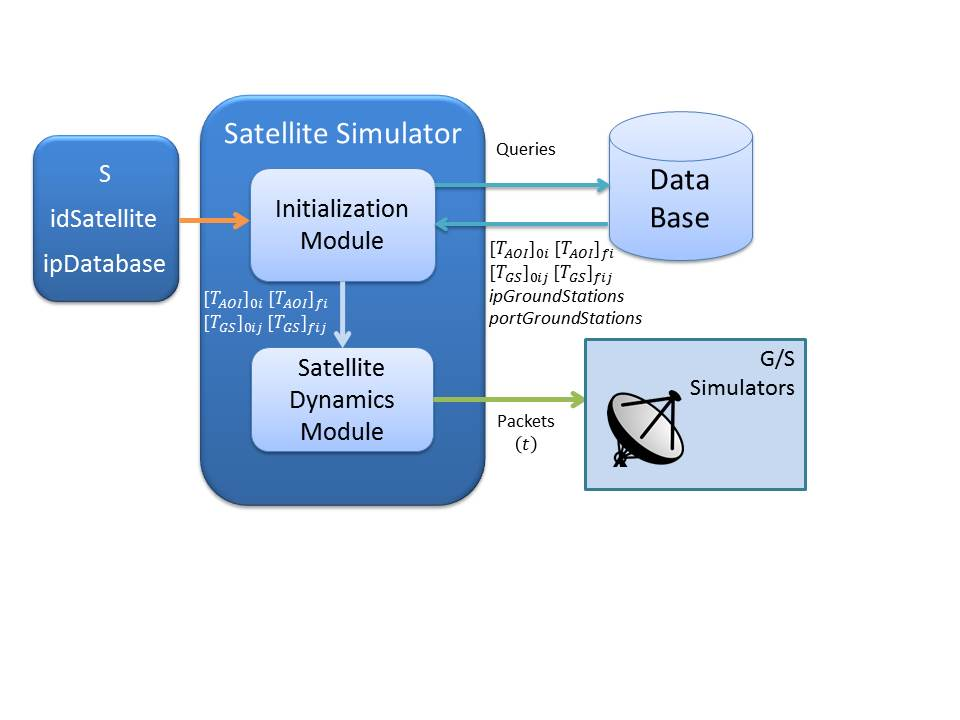
\includegraphics[width=0.7\textwidth]{spaceSystemSimulator/sat-simulator-architecture.jpg}
\caption{Satellite Simulator Architecture}
\label{fig:sss-sat-simulator-architecture}
\end{center}
\end{figure}

\paragraph{Satellite Simulator Workflow}~\\
\label{par:satellite-workflow}
The \emph{Satellite Simulator} starts the execution following these steps:
\begin{enumerate}
\item The \emph{Initialization Module} obtains \emph{S}, \emph{idSatellite} and \emph{ipDatabase}.
\item Then, the \emph{Initialization Module} makes queries on the database to obtain all the required satellite data for current scenario: $[T_{GS}]_{0ij}$, $[T_{GS}]_{fij}$,  $[T_{AOI}]_{0i}$ and $[T_{AOI}]_{fi}$. The queries made to the database contain the particle “order by timeInZone” column. This means that the database returns the $[T_{GS}]_{0ij}$ times in ascending order. Other query gets the \emph{ipGroundStations} and \emph{portGroundStations} of every \emph{Ground Station Simulator}.
\item Schedule of data download: the \emph{Satellite Simulator} schedules the data download from the \emph{Satellite Simulator} to the \emph{Ground Station Simulators} (see Section~\ref{subpar:shedule-process}).
\item When all the communications between the \emph{Satellite Simulator} and the \emph{Ground Station Simulators} have been scheduled in time, the \emph{Satellite Simulator} starts \emph{Satellite Dynamics Module}.
\item When the last scheduled task has been executed, the \emph{Satellite
    Simulator} finishes the execution.
\end{enumerate}
Figure~\ref{fig:sss-sat-simulator-workflow} shows the process explained above. The diagram also shows the
interactions with the other subsystems (see also Figure~\ref{fig:sss-sat-simulator-architecture}). Figure~\ref{fig:sss-sat-simulator-workflow} also shows the inputs for the \emph{Satellite Simulator} and the outputs after its execution. These outputs are the packets in time sent to the ground stations and a log file that contains the information about the execution. In orange the inputs to the \emph{Satellite Simulator} are represented, in green the transitions in the workflow and in blue the outputs.

\begin{figure}[!h]
\begin{center}
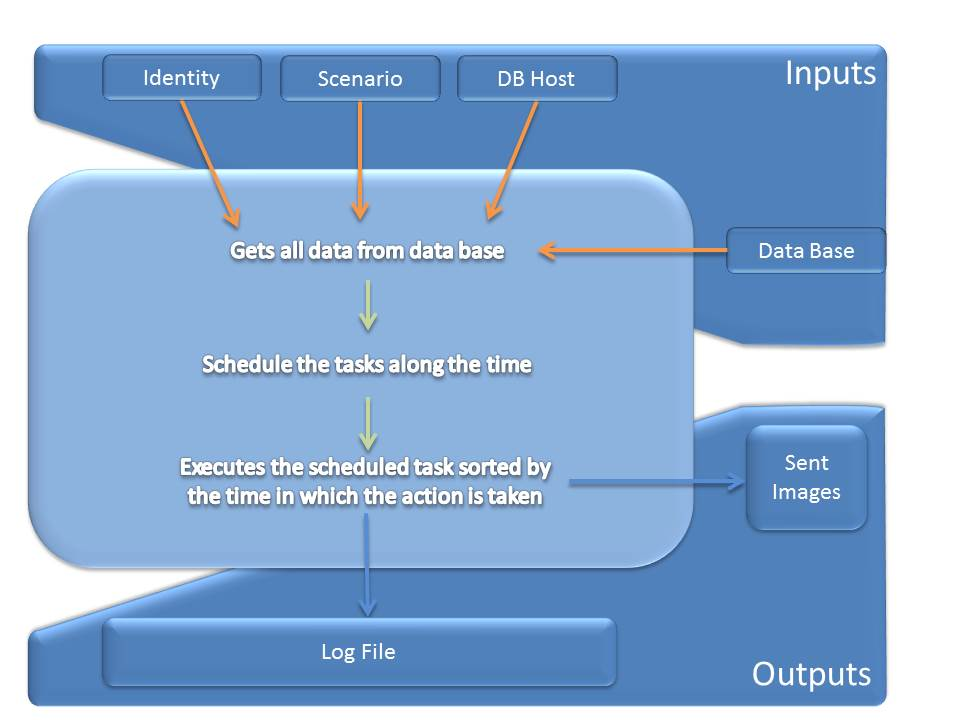
\includegraphics[width=0.8\textwidth]{spaceSystemSimulator/sat-simulator-workflow.jpg}
\caption{Satellite Simulator Workflow}
\label{fig:sss-sat-simulator-workflow}
\end{center}
\end{figure}

\subparagraph{Schedule of data download process}~\\
\label{subpar:shedule-process}
\textbf{Definitions:}

Regarding the images download process, the satellites should download at
$160~Kbps$ to the ground station. In \vw we have a limited bandwidth at
$100~Kbps$. To solve this problem we designed several types of packets (with one
byte size), which are sent between \vw nodes instead of real satellite
imagery. The packets contain all the metadata of the images: \emph{AOI}, non \emph{AOI}, area
between visibility cones.  These packets are the following:
\begin{itemize}
\item \emph{Packet ``U'':} The transmission of this packet means that the satellite sends \emph{AOI} images at $98.6~Mbps$ and \emph{non AOI} images at $64.1~Mbps$.
\item \emph{Packet ``I'':} The transmission of this packet means that the satellite sends \emph{non AOI} images at $160~Mbps$.
\item \emph{Packet ``B'':} The transmission of this packet means that the
  satellite sends \emph{AOI} images at $160~Mbps$.
\end{itemize}

To schedule the data download process the following functions were defined:
\begin{itemize}
\item \emph{NotInterestingZone:}  it represents the non \emph{AOI} area that is
  being recorded by the satellite when it is inside a visibility cone. It
  creates a new connection with the \emph{Ground Station Simulator} and
  transmits packets type ``I''. The inputs of this function are the following:
\begin{itemize}
\item \emph{ipGroundStation:} \emph{IP address} of the \emph{Ground Station Simulator}.
\item \emph{t\_ini:} start time in which the function is executed.
\item \emph{t\_end:} end time in which the function is finished.
\end{itemize}

The function has implemented the pseudo-code in Listing~\ref{code:sss-notinterestingzone}.

\begin{listing}[
  float=h!,
  caption  = {Pseudocode of \emph{NotInterestingZone} function},
  label    = code:sss-notinterestingzone,
style=customc]
function NotInterestingZone (t_ini,t_end,ipGroundStation):
offset <-0 //deviation of the normal time
socket <- connect(ipGroundStation) //connection with the GS
current_t <- time() //get the current system time
penal_times <-0 // times that time function is called
time_penalty <- time that time() costs
while (current_t  <  t_end + offset):
	Socket.send('I')
	Penal_times <- penal_times+2
	Offset = penal_times * time_penalty
	Time.sleep(0.2-(time()-t_temp))
	t_temp <- time()
end while
socket.close()
\end{listing}

\item \emph{InterestingZone:} It represents the \emph{AOI} area that is being
  recorded by a satellite when it is inside a visibility cone. It creates a new
  connection with the \emph{Ground Station Simulator} and transmits packets type
  ``U'' and ``B''. The inputs of this function are the following:
\begin{itemize}
\item \emph{ipGroundStation:} \emph{IP address} of the \emph{Ground Station Simulator}.
\item \emph{t\_ini:} start time in which the function is executed.
\item \emph{t\_end:} end time in which the function is finished.
\item \emph{offset\_time:} It is the difference $([T_{GS}]_{0ij}- [T_{AOI}]_{0i} )*CR$.
\end{itemize}
The function has implemented the  pseudo-code in Listing~\ref{code:sss-interestingZone}:
\begin{listing}[
  float=h!,
  caption  = {Pseudocode of \emph{InterestingZone} function},
  label    = code:sss-interestingZone,
  style=customc]
function InterestingZone (t_ini,t_end,offset_time,ipGroundStation):
offset <-0 //deviation of the normal time
socket <- connect(ipGroundStation) //connection with the GS
current_t <- time() //get the current system time
penal_times <-0 // times that time function is called
time_penalty <- time that time() costs

while (current_t <  t_ini+offset_time + offset):
	socket.send('B')
	penal_times <- penal_times+2
	offset = penal_times * time_penalty
	time.sleep(0.2-(time()-current_t))
current_t<- time()
end while
while (current_t <  t_end + offset):
	socket.send('U')
	penal_times <- penal_times+2
	offset = penal_times * time_penalty
	time.sleep(0.2-(time()-current_t))
current_t<- time()
end while
socket.close()
\end{listing}

\item \emph{OutOfVisibility:} The satellite is not in the visibility cone of a
  ground station, the satellite follows the orbit until it enters into a
  visibility cone. It does not transmit any packet. The inputs of this function
  are the following:
\begin{itemize}
\item \emph{t\_ini:} start time in which the function is executed.
\item \emph{t\_end:} end time in which the function is finished.
\end{itemize}
The function has implemented the pseudo-code in Listing~\ref{code:sss-outofvisibility}:

\begin{listing}[
  float=h!,
  caption  = {Pseudocode of \emph{OutOfVisibility} function},
  label    = code:sss-outofvisibility,
style=customc]
function OutOfVisibility (t_ini,t_end):
offset <-0 //deviation of the normal time
socket <- connect(ipGroundStation) //connection with the GS
current_t <- time() //get the current system time
penal_times <-0 // times that time function is called
time_penalty <- time that time() costs
while (current_t  <  t_end + offset):
	penal_times <- penal_times+2
	offset = penal_times * time_penalty
	time.sleep(0.2-(time()-t_temp))
	t_temp <- time()
end while
socket.close()

\end{listing}

\end{itemize}

\textbf{Scheduling process:}

This process consists of the scheduling all the satellite interactions with the
ground stations. This is done as follows:
\begin{enumerate}

\item If the area the satellite is flying over is not \emph{AOI}, the function
  \emph{NotInterestingZone} is scheduled to be executed as follows:
  \mbox{\emph{NotInterestingZone(ipGroundStation, $[T_{GS}]_{0ij}$, $[T_ {GS}]_{fij}$)}}. The
  function \emph{OutOfVisibility} is scheduled to be executed as follows:
  \emph{OutOfVisibility($[T_{GS}]_{fij}$, $[T_{GS}]_{(0i(j+1)})$)}, and the scheduling process finishes.
\item Otherwise three cases can take place:
\begin{itemize}
\item If $[T_{AOI}]_{0i}< [T_{GS}]_{0ij} || [T_{AOI}]_{0i}= [T_{GS}]_{0ij}$ the
  function \emph{InterestingZone} is scheduled to be executed as follows:
  \emph{InterestingZone(ipGroundStation, $[T_{GS}]_{0ij}$, $[T_{AOI}]_{fij}$ ,
    offset\_time)}. It is always considered that $[T_{AOI}]_{fi} > [T_{GS}]_{fij}$.
\item If $[T_{AOI}]_{0i}>[T_{GS}]_{0ij}$, first, the function \emph{NotInterestingZone}
  is scheduled to be executed as follows:
  \emph{NotInterestingZone(ipGroundStation, $[T_{GS}]_{0ij}$, $[T_{AOI}]_{0ij}$)}; and
  second, the function \emph{InterestingZone} is scheduled to be executed as
  follows: \emph{InterestingZone(ipGroundStation, $[T_{AOI}]_{0ij}$, $[T_{AOI}]_{fij}$,
    0)}.
\end{itemize}
\item The \emph{NotInterestingZone} function is scheduled to be executed as\\ \mbox{\emph{NotInterestingZone(ipGroundStation,}}\emph{$[T_{AOI}]_{fij}$, $[T_{GS}]_{fij}$)}.
\item The function \emph{OutOfVisibility} is scheduled to be executed as
  follows: \emph{OutOfVisibility($[T_{GS}]_{fij}$, $[T_{GS}]_{(0i(j+1)})$)}, and
  the scheduling process finishes.
\end{enumerate}

Figure~\ref{fig:sss-sheduling-process} graphically shows the scheduling process explained above.


\begin{figure}[!h]
\begin{center}
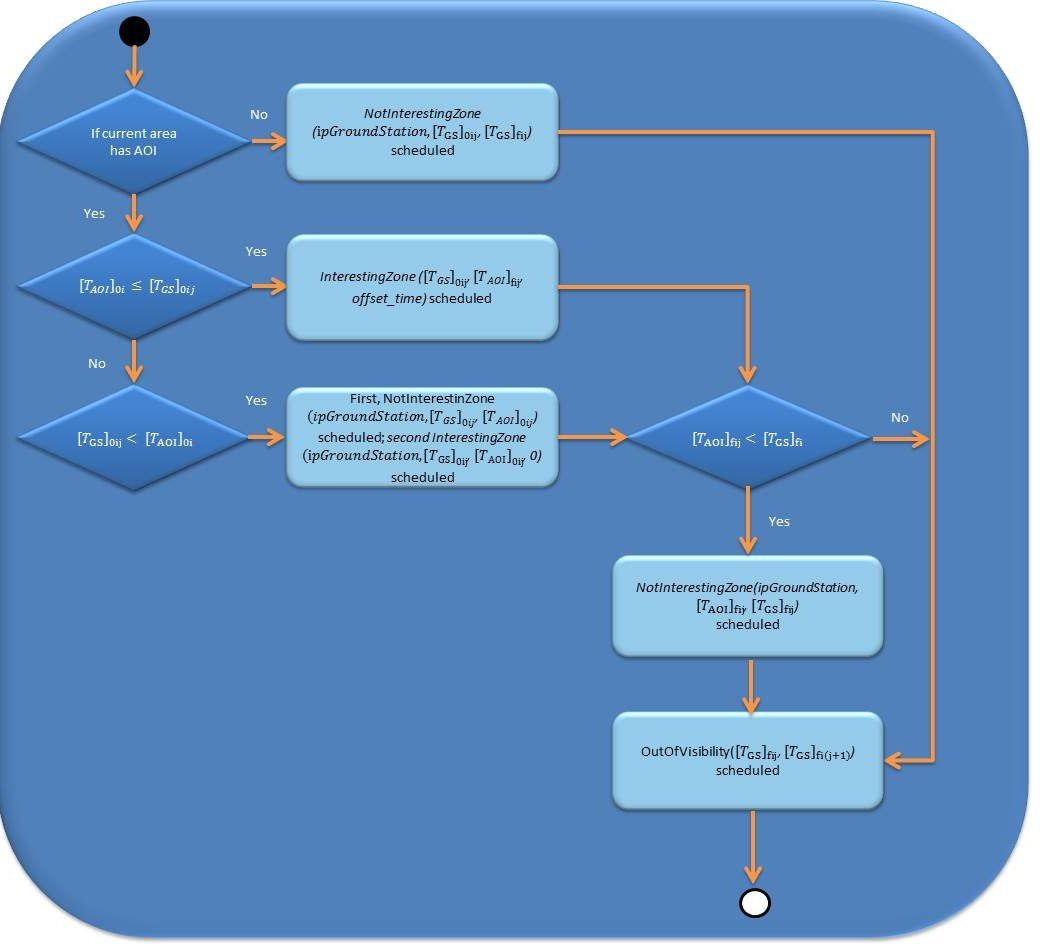
\includegraphics[width=1\textwidth]{spaceSystemSimulator/sheduling-process.jpg}
\caption{Sheduling Process on the Satellite Simulator}
\label{fig:sss-sheduling-process}
\end{center}
\end{figure}


The activity diagram in \emph{UML} format of the \emph{Satellite Simulator} is
depicted in Figure~\ref{fig:sss-satellite-activity}.

\begin{figure}[!h]
\begin{center}
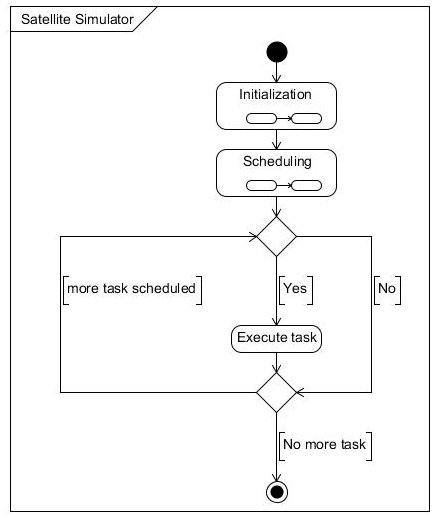
\includegraphics[width=0.6\textwidth]{spaceSystemSimulator/sat-simulator-activity.jpg}
\caption{Satellite Simulator Activity Diagram}
\label{fig:sss-satellite-activity}
\end{center}
\end{figure}

\paragraph{Satellite Simulator Implementation}
\label{par:sat-simulator-implementation}~\\

The implementation was done in Python 2.7. The python's libraries needed to
implement the software are listed in Table~\ref{table:sss-satellite-libraries}.



\begin{table}[h]
  \centering
  {\small
  


\begin{tabular}{p{.2\textwidth}p{.2\textwidth}}
  \tabheadformat
  \tabhead{Python Library}   &
  \tabhead{Function}\\
\hline
\textit{Sys}         & System library \\
\hline
\textit{OS}         & Operative system interactions supply \\
\hline
\textit{Sched}         & Library that allow the Satellite Simulator to schedule the task along  the time \\
\hline
\textit{Time}         & For managing the time \\
\hline
\textit{Socket}         & Library for creating and establishing connections with other host \\
\hline
\textit{Pdb}         &  Used for debugging the software\\
\hline
\textit{Logging}         &Log      \\
\hline
\end{tabular}


% Local variables:
%   coding: utf-8
%   ispell-local-dictionary: "castellano8"
%   TeX-master: "main.tex"
% End:

  }
  \caption{Satellite Simulator's Python Libraries}
  \label{table:sss-satellite-libraries}
\end{table}

When we installed Python, all the libraries were installed with the exception of ``MySQLdb'', which was manually installed.

Furthermore, STK provided the time in the next formats:
\begin{itemize}
\item \emph{UTCG format:} Universal Time Coordinated in Gregorian format.
\item \emph{Format in seconds:} total of seconds
\end{itemize}
They are the absolute time from the beginning of the constellation simulation in
the STK software. In the data base, the stored times are implemented in
seconds. However to simulate a scenario in real time is too long. It can be
shortened by computing a relative time $(T_r)$:
\begin{equation}\label{eq:TR}
	T_r=T/n
\end{equation}

where $T$ is the absolute time and $n$ a factor that scales the absolute time to
reduce the execution time of the experiment. In preliminary simulations we used
$n=10$, although during the experiment execution stage this will be evaluated
and probably changed. The Table~\ref{table:sss-scenario-relative-time} shows the absolute times and relative times for each scenario duration.


\begin{table}[h]
  \centering
  {\small
  


\begin{tabular}{p{.2\textwidth}p{.2\textwidth}p{.2\textwidth}}
  \tabheadformat
  \tabhead{Scenario}   &
  \tabhead{Absolute Time}&\tabhead{Relative Time}\\
\tabheadformat
& \tabhead{$(T_0,T_f)$} & \tabhead{$(T_{r0}, T_{rf})$}\\
\tabheadformat
&\tabhead{(Seconds)}& \tabhead{(Seconds)}\\
\hline
\textit{Scenario 1: Emergencies – Lorca Earthquake (Spain)}         & (63638, 63661)& (6363.8, 6366.1)\\
\hline
\textit{Scenario 2: Infrastructure monitoring. Affection in railway infrastructures by sand movement in desert areas (Spain)}         & (54060, 54753) & (5406.0, 5475.3)\\
\hline
\textit{Scenario 3: Land Management – South West of England}         & (62480, 63865)& (6248.0, 6386.5) \\
\hline
\textit{Scenario 4: Precision Agriculture – Argentina}         & (78461, 84999) & (7846.1, 8499.9) \\
\hline
\textit{Scenario 5: Basemaps – Worldwide}         & (0, 86400) & (0, 8640.0)\\
\hline
\end{tabular}


% Local variables:
%   coding: utf-8
%   ispell-local-dictionary: "castellano8"
%   TeX-master: "main.tex"
% End:

  }
  \caption{Scenarios relative times}
  \label{table:sss-scenario-relative-time}
\end{table}


\paragraph{Execution}~\\
\label{par:sat-simulator-execution}
To execute the \emph{Satellite Simulator Software} the following dependencies are
required:
\begin{itemize}
\item Operative System based in \emph{GNU Debian}.
\item Python v.2.7
\item Python packages (Table~\ref{table:sss-satellite-libraries}).
\item Ethernet interface for the network connection.
\item Connectivity with the data base located in \bonfire through the network.
\end{itemize}
The \satss software is developed in a multiplatform language, but it is restricted to be executed in \emph{UNIX} operative systems because there are many dependencies with some packages and the file system.

The execution of the satellite software has to be done as \emph{super-user} in
\emph{UNIX}. It is executed with the following command line:
\begin{itemize}
\item[>] python~satellite.py~<IDSAT>~<SCENARIO>~<DBHOST>~[LOGLEVEL]
\end{itemize}

where:
\begin{itemize}
\item \emph{IDSAT} is the satellite identity. This value must be an integer.
\item \emph{SCENARIO} is the scenario number to simulate. Must be an integer.
\item \emph{DBHOST} is the host where the data base is located. Must be a hostname or an \emph{IP address}.
\item \emph{LOGLEVEL} is the level of log that the software will show. The values can be: INFO, DEBUG. This parameter is optative. By default its value is INFO.
\end{itemize}

\subsection{Ground Station System Simulator}

In this section, the implementation and the architecture of the \emph{Ground Station Simulator} is described. The \gsss reproduces the behaviour of the set of 12 ground stations by replicating 12 times a \emph{Ground Station Simulator} that renders individual ground stations behaviour.

The \gsss is a manager that executes 12 \emph{Ground Station Simulators}. The
\gsss requires the scenario number and the \emph{IP address} of the database as
an input and executes the \emph{Ground Station  Simulators} by providing them
the specific identity of the ground station \emph{(idGroundStation)}, number of
the scenario \emph{(S)} and \emph{IP address} of the distributed database
\emph{(ipDatabase)}.

\subsubsection{Ground Station Simulator}

The functions of the ground stations are the following:
\begin{itemize}
\item To receive the images sent by the satellites.
\item To create the files with the raw images that the \emph{Orchestrator} will
  download for processing and publishing in the \emph{Archive and Catalogue} subsystem.
\end{itemize}

The \emph{Ground Station Simulator} software is common for all the ground stations, but it is parameterized to define each of them, similarly to the \emph{Satellite Simulator}.

The \emph{Ground Station Simulator} is constituted by the following components:
\begin{enumerate}
\item \emph{Initialization Module:} This module obtains the following parameters
  and   initializes the \emph{Ground Station Simulator}:
\begin{itemize}
\item \emph{S:} the number of the scenario to simulate.
\item \emph{idGroundStation:} identification number of the ground station (1 to 12).
\item \emph{ipDatabase:} \emph{IP address} of the database.
\end{itemize}

Once obtained the previous parameters, the \emph{Initialization Module} connects
with the database and fetches the name of the ground station. Also, a query to
update the \emph{IP address} and port of the \emph{Ground Station Simulator} server is sent to the database.
\item \emph{Ground Station Dynamics Module:} This module represents the dynamics and associated parameters of the ground station. It requires \emph{S}, \emph{ipDatabase} and \emph{idGroundStation}.
\end{enumerate}
Figure~\ref{fig:sss-ground-station-architecture} shows the relation between the previous modules.

\begin{figure}[!h]
\begin{center}
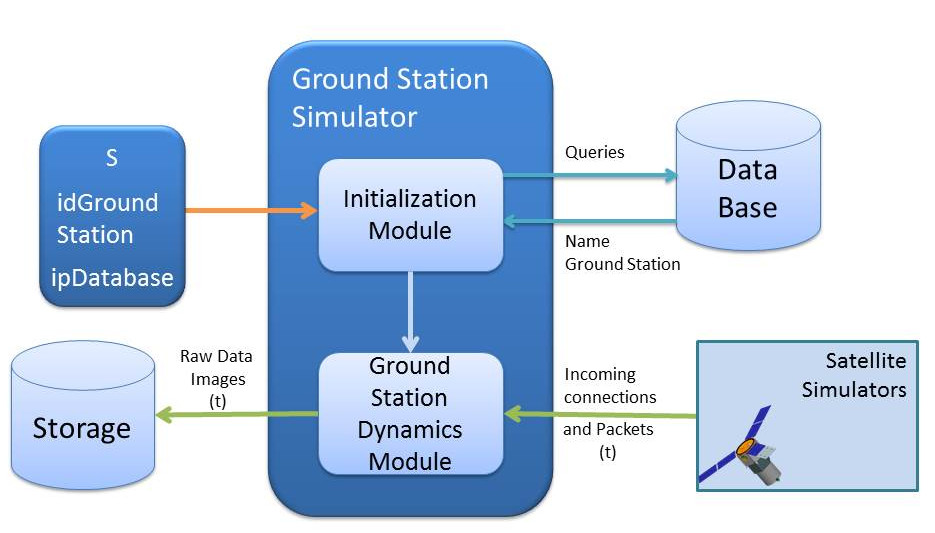
\includegraphics[width=0.7\textwidth]{spaceSystemSimulator/ground-station-architecture.jpg}
\caption{Ground Station Simulator Architecture}
\label{fig:sss-ground-station-architecture}
\end{center}
\end{figure}

\subsubsection{Ground Station Simulator Workflow}

The \emph{Ground Station Simulator} starts the execution following these steps:
\begin{enumerate}
\item The \emph{Initialization Module} obtains \emph{S}, \emph{idGroundStation} and \emph{ipDatabase}.
\item Then, the \emph{Initialization Module} queries on the database for the
  name of the ground station and for updating the \emph{IP address} and
  \emph{port} of the \emph{Ground Station Simulator}.
\item The \emph{Ground Station Dynamics Module} starts:
\begin{itemize}
\item A network socket\footnote{Network socket is an endpoint of an inter-process communication flow across a computer network. Most of the communications between computers are based on the Internet Protocol using network sockets.}  is created for listening input connections from \emph{Satellite Simulators}.
\item Every time a satellite enters into the visibility cone of the ground station a connection between a \emph{Satellite Simulator} and the \emph{Ground Station Simulator} is created. Note that if several satellites are in the same visibility cone, the \emph{Ground Station Simulator} opens a connection for each \emph{Satellite Simulator}, and that the \emph{Ground Station Simulator} can listen to new connections if new satellites enter into the visibility cone.
\item The \emph{Ground Station Simulator} creates a new process to keep the previous connection or connections (if there are more than one satellite in the visibility cone) open.
\item The new process or processes receive the packets sent by the \emph{Satellite Simulators}.
\item Once the transmission between the \emph{Satellite Simulators} and the \emph{Ground Station Simulator} finished the connections are closed.
\item Then the received packets are counted and classified by type (see Section~\ref{subpar:shedule-process}):
\begin{itemize}
\item \emph{Packet ``U'':} $98.6~Mb$ are added to the \emph{AOI} buffer and $64.1~Mb$ are added to the \emph{non AOI} buffer in the \emph{Ground Station Simulator}.
\item \emph{Packet ``I'':} $160~Mb$ are added to the \emph{non AOI} buffer in the \emph{Ground Station Simulator}.
\item \emph{Packet ``B'':} $160~Mb$ are added to the \emph{AOI} buffer in the
  \emph{Ground   Station Simulator}.
\end{itemize}
After classifying the packets, the new processes finish.
\item The \emph{AOI} images and \emph{non AOI} images are created in the \emph{Ground Station  Simulator}.
\end{itemize}
\item The \emph{Ground Station Simulator} server ends when it receives the \emph{SIGINT} signal.
\end{enumerate}

Figure~\ref{fig:sss-ground-station-workflow} shows the process explained above. The diagram also shows the interactions with the other subsystems (see Figure~\ref{fig:sss-ground-station-architecture}). Figure~\ref{fig:sss-ground-station-workflow} shows the inputs for the \emph{Ground Station Simulator} and the outputs after its execution. These outputs are the Raw Images in time created and a log file that contains the information about the execution.

\begin{figure}[!h]
\begin{center}
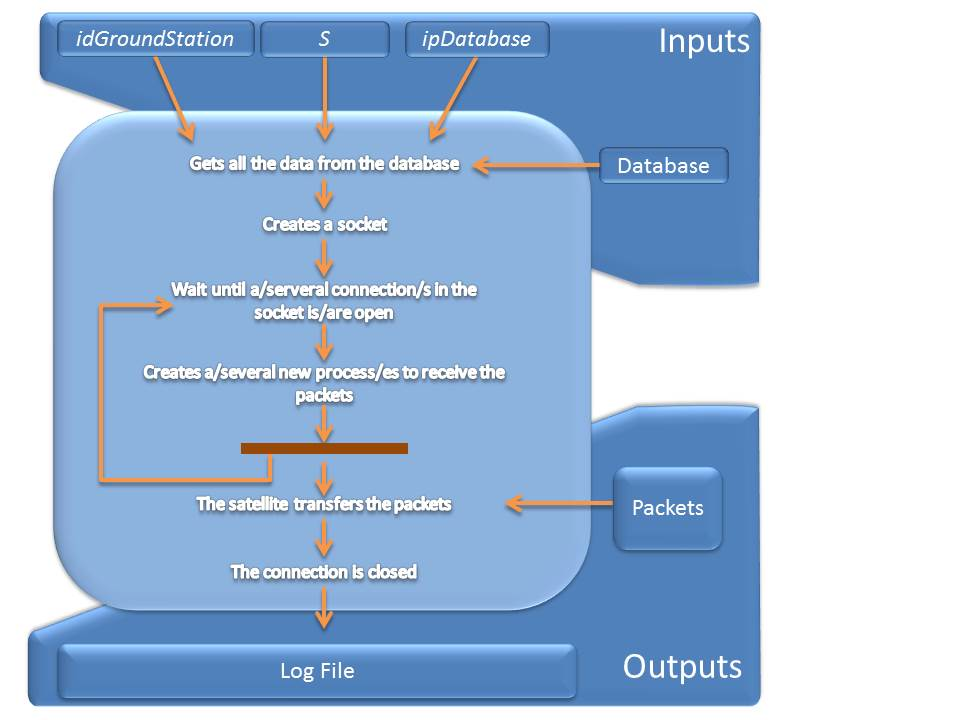
\includegraphics[width=0.85\textwidth]{spaceSystemSimulator/ground-station-workflow.jpg}
\caption{Ground Station Simulator Workflow}
\label{fig:sss-ground-station-workflow}
\end{center}
\end{figure}

The activity diagram of the Ground Station Simulator in UML format  is depicted
in Figure~\ref{fig:sss-ground-station-activity}.

\begin{figure}[!h]
\begin{center}
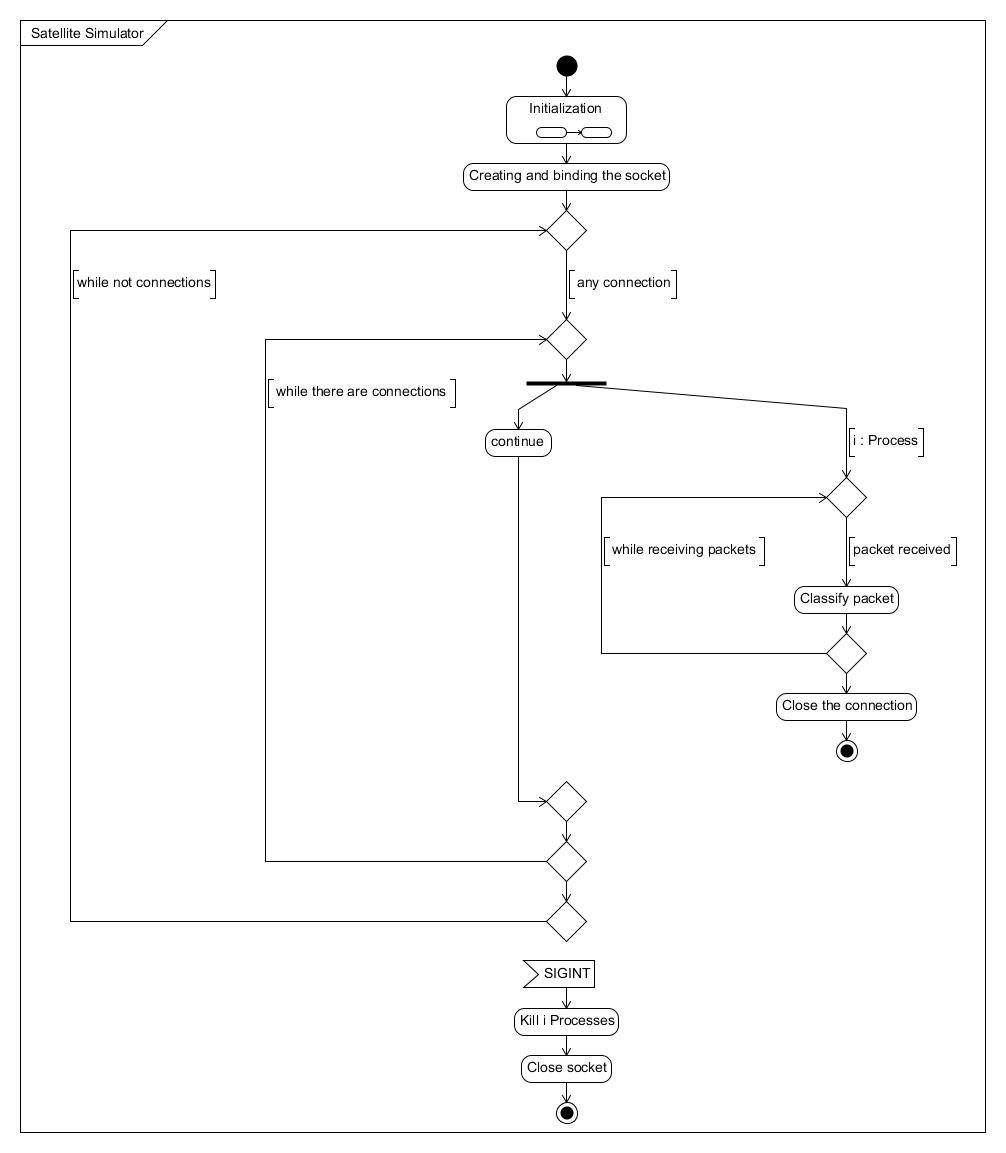
\includegraphics[width=0.9\textwidth]{spaceSystemSimulator/ground-station-activity.jpg}
\caption{Ground Station Simulator Activity Diagram}
\label{fig:sss-ground-station-activity}
\end{center}
\end{figure}

\paragraph{Implementation}\label{par:sss-ground-implementation}~\\
The implementation was done in Python 2.7, using the libraries described in
Table~\ref{table:sss-ground-libraries}.

\begin{table}[h]
  \centering
  {\small
  


\begin{tabular}{p{.2\textwidth}p{.2\textwidth}}
  \tabheadformat
  \tabhead{Python Library}   &
  \tabhead{Function}\\
\hline
\textit{Sys}         & System library \\
\hline
\textit{OS}         & Operative system interactions supply \\
\hline
\textit{Sched}         & Library that allow the Satellite Simulator to schedule the task along  the time \\
\hline
\textit{Time}         & For managing the time \\
\hline
\textit{Socket}         & Library for creating and establishing connections with other host \\
\hline
\textit{Pdb}         &  Used for debugging the software\\
\hline
\textit{Logging}         &Log      \\
\hline
\end{tabular}


% Local variables:
%   coding: utf-8
%   ispell-local-dictionary: "castellano8"
%   TeX-master: "main.tex"
% End:

  }
  \caption{Ground Station Simulator Python Libraries}
  \label{table:sss-ground-libraries}
\end{table}

\paragraph{Execution}\label{par:sss-ground-execution}~\\
To execute the Ground Station Simulator Software the following dependencies are
required:
\begin{itemize}
\item Operative System based in \emph{GNU Debian}.
\item Python v.7.
\item Python packages: (shows in Table~\ref{table:sss-ground-libraries}).
\item Ethernet interface for the network connection.
\item Connectivity with the data base located in \bonfire through the network.
\end{itemize}

The \emph{Ground Station Simulator} is developed in a multiplatform language, but it is restricted to be executed in \emph{UNIX} operative systems because there are many dependencies with some packets and the file system.

The software also needs to know the \emph{IP addresses} assigned to its Ethernet interface. If this interface is not connected, the software looks for the WLAN0 interface. This information is accomplished from the \emph{UNIX} file ``/etc/hosts''.

The execution of the satellite software must be done as sudo user as follows:
\begin{itemize}
\item[>]python~groundstation.py~<IDSAT>~<SCENARIO>~<DBHOST>~[LOGLEVEL]
\end{itemize}

where:
\begin{itemize}
\item \emph{IDSAT} is the ground station identity. This value must be an integer.
\item \emph{SCENARIO} is the scenario to simulate. It must be an integer.
\item \emph{DBHOST} is the host where the data base is located. It must be a hostname or an \emph{IP address}.
\item \emph{LOGLEVEL} is the level of log that the software will show. The
  values can be: INFO, DEBUG. This parameter is optative. Its value is INFO by default.
\end{itemize}



\section{Implementation in Virtual Wall}
\label{sec:impl-vw}
% In this section, the implementation is introduced indicating the testbeds involved in it and the required steps for the implementation.

% Fistly, the implementation of the \sss in \vw is depicted. The designed topology and the new
% modified topology (different to the designed one) are depicted because of the handicaps of
% the hardware during the implementation. Then, nodes reservation is
% explained and detailed. Finally, the scripts included in each type of
% node are described before the presentation of the execution.

% The next section is dedicated to the implementation of the software
% developed in the \bonfire testbed. Nodes reservation is firstly
% depicted. Architecture and setup are also explained. And again, the
% scripts for each node setup are included before the description of the
% execution.

% Finally, the integration between \vw and \bonfire is described.

% Section 6 is devoted\ to\ describe the\ demonstration\ of the\ GEO-Cloud
% experiment prepared for the European Commission in June 2014.

In this section, the implementation of the \sss in \vw is explained. First, the designed
topology and the new modified topology (different to the design one) are layed out because
the handicaps of the hardware during the implementation. Then, nodes reservation is
explained and detailed. Finally, the scripts included in each type of node are described
before the presentation of the execution.


% \bigskip

% Finally, section 7 provides\ the main\ conclusions.


\subsection{Topology network}

The \sss is comprised of the
following modules:
\begin{itemize}
\item The \emph{Satellite System Simulator}
\item The \emph{Ground Station System Simulator}
\end{itemize}
The topology network designed is depicted in Figure~\ref{fig:impl-topology-vw}.

\begin{figure}[!h]
\hspace{-1cm}
\begin{center}
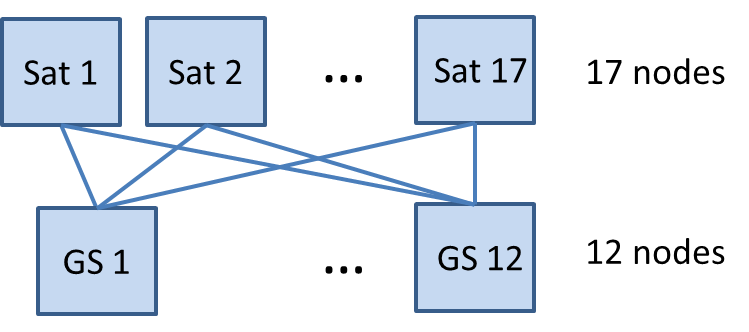
\includegraphics[width=0.68\textwidth]{implementationVWBF/gs-sat.png}

\caption{Topology Network in \vw}
\label{fig:impl-topology-vw}
\end{center}
\end{figure}



The previous topology network involves Sat nodes to have 12 connections with the GS nodes; and GS nodes 17 connections with Sat nodes plus one connection with the \bonfire cloud.

The nodes in \vw have a limitation of 5 physical connections. To deploy the previous
topology we adapted the \sss software to establish those connections by software. This was
done by making the \satss flexible to connect with any ground station from GS1 to GS12. 

The solution was to multiply the \satss by 3 and connect 4 ground stations to each \satss. This ensures the same performance and dynamics of the previous topology network described in Figure~\ref{fig:impl-topology-vw}, and the only thing it changes is the software.

The \sss implemented in \vw is depicted in Figure~\ref{fig:impl-nodes-vw}.

\begin{figure}[!h]
\begin{center}
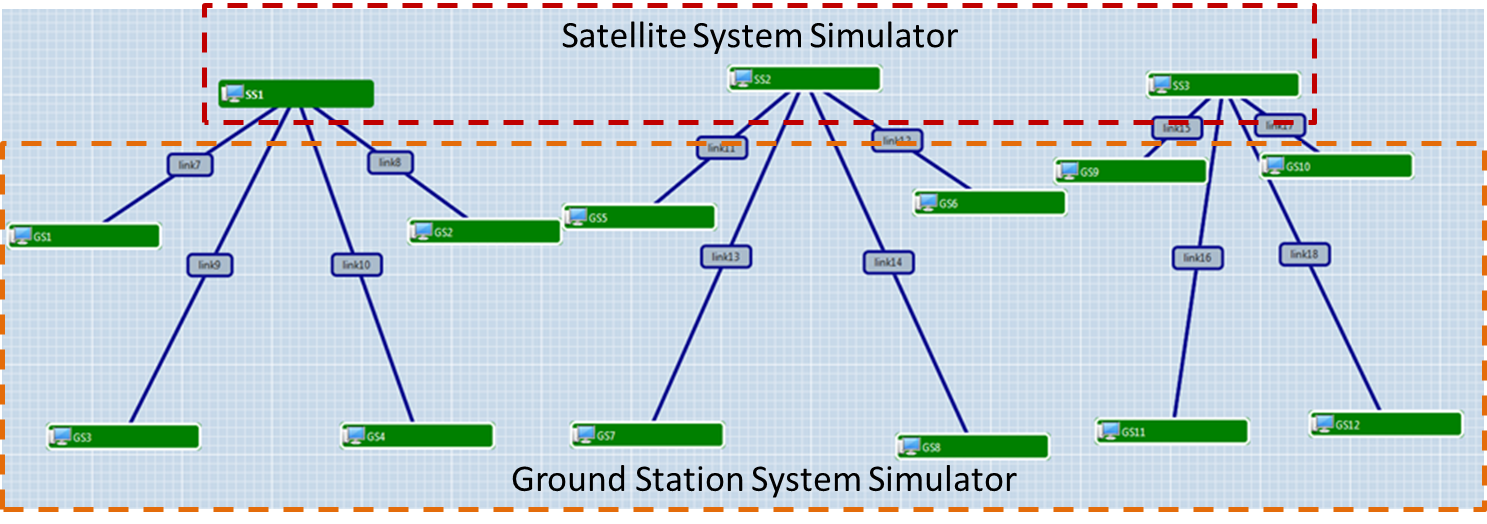
\includegraphics[width=0.9\textwidth]{implementationVWBF/nodes-vw.png}

\caption{Topology Network of the \satss}
\label{fig:impl-nodes-vw}
\end{center}
\end{figure}



\subsubsection{Nodes Reservation and Setup}

The \sss is then constituted by 15 ``Generic nodes'' in \vw 1 (The \vw
testbed is composed by two sets of machines, \vw 1 and \vw 2). The configuration of the experiment makes the provisioning of ``any available node'',
which is more flexible in case a node is being used in other experiment (see Figure~\ref{fig:creating-node-jfed}). The links between SS \emph{(Satellite Simulators)} and GS \emph{(Ground Stations Simulators)} nodes
are \ac{TCP}. The definition of the dependencies and the commands that will be installed at
setup is defined in \emph{JFed} using a \emph{Rspec} specification. This specification includes some
bash commands or instructions that will execute after reservation automatically.


\begin{figure}[!h]
\begin{center}
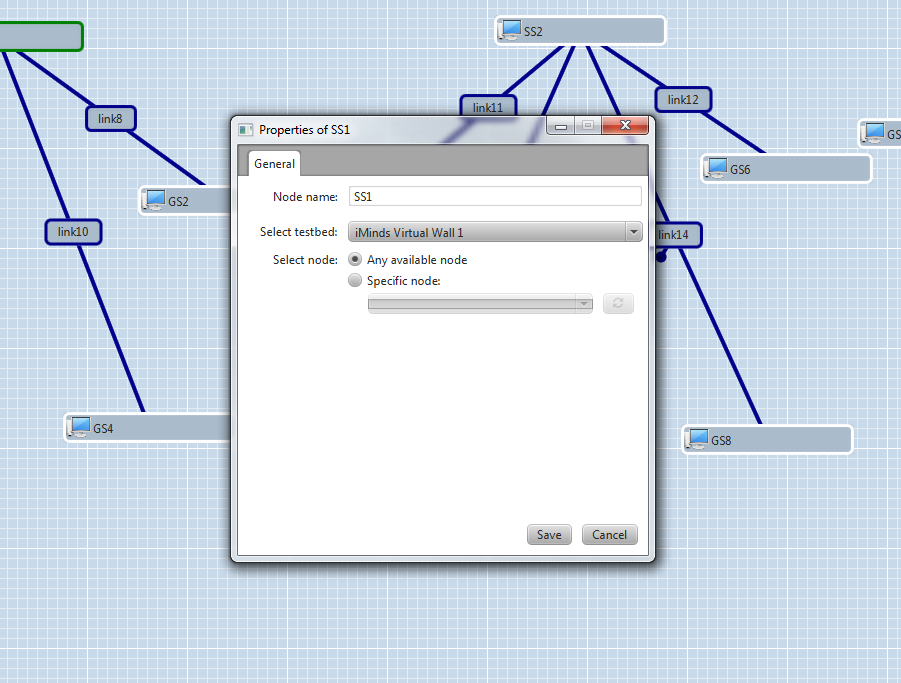
\includegraphics[width=0.9\textwidth]{implementationVWBF/creating-node-jfed.png}

\caption{Configuration of \vw nodes}
\label{fig:creating-node-jfed}
\end{center}
\end{figure}


\paragraph{Satellite Simulator Nodes Setup}~\\
The configuration of the nodes is done by using \emph{JFed Rspec Experiment}. The
setup steps are the following:
\begin{itemize}
\item To configurate a gateway for obtaining Internet connectivity and installing the
  needed libraries.
\item To update the system.
\item Once the update is finished, dependencies can be installed.
\item As the simulators require a connection with a database, the \emph{MySQL} library is
  also required. 
\item Source is downloaded from Google Drive where is located.
\end{itemize}

The script that perform the above is showed in Listing~\ref{code:impl-rspec-sat-sim}.

\lstset{float=h!,caption={Rspec specification for \emph{Satellite Simulators}},style=customc,numbers=left,label={code:impl-rspec-sat-sim}}
\lstinputlisting[firstline=2,lastline=14]{../../source/vw/Description.rspec}



Where <<google\_drive\_host\_address>> is the address of the Google Drive URI in which the scripts are located.

The \emph{Database} is located in \bonfire and it has an \emph{IP address} that can change. In order to
obtain that \emph{IP address} and include it in the \emph{Satellite Simulator}, a simple script to
acquire the \emph{IP address} of the database was developed \emph{push\_dbIP.sh}.
Listing~\ref{code:impl-script-ipdb} contains the script.

\lstset{float=h!,caption={Bash script to write the Database's \emph{IP address} on a file},style=customc,numbers=left,label= code:impl-script-ipdb}
\lstinputlisting{../../source/vw/push_ip.sh}

The execution of the \emph{push\_dbIP.sh} script acquires the \emph{IP address} of the database and includes it in the file \emph{ipdb}, created by \emph{push\_dbIP.sh}.
Finally, the node is perfectly configured to proceed with the installation of the
\emph{Satellite Simulator}. The software of the simulator has been archived too in
\emph{Google Drive}. The software is acquired and it can now be executed in the node.


\subsubsection{Ground Station Simulator Nodes Setup}


The \emph{Ground Station Simulators} software is developed under Python. The steps of
setup are the following:
\begin{itemize}
\item To configurate a gateway for obtaining Internet connectivity and installing the
  needed libraries.
\item To update the system.
\item Once the update is finished, dependencies can be installed.As occurred with the SS nodes, the update and the installation of Python and MySQL are required.
\item As the simulators require a connection with a database, the \emph{MySQL} library is
  also required. 
\item Source is downloaded from Google Drive where is located.
\item The database IP address is added to \emph{ipdb} file.
\item  The raw data is located in Google Drive too.  
\item The GS nodes are required to open an \emph{FTP} to be accessed from the
\emph{Orchestrator} in \bonfire. The \emph{FTP} is configured by executing the
\emph{install\_ftp.sh} file. This file content is in Listing~\ref{code:impl-ftp-installation}.  
\end{itemize}

The script that perform the above is showed in Listing~\ref{code:impl-rspec-gs-sim}.

\lstset{float=h!,caption={Rspec specification for \emph{Ground Station Simulators}},style=customc,numbers=left,label={code:impl-rspec-gs-sim}}
\lstinputlisting[firstline=64,lastline=78]{../../source/vw/Description.rspec}


\lstset{float=h!,caption={FTP server installation},style=customc,numbers=left,label={code:impl-ftp-installation}}
\lstinputlisting{../../source/vw/install_ftp.sh}


Through the FTP connection the raw data will be transferred from the GS nodes to the BonFIRE cloud. 

The execution of the Satellite Simulators and the Ground Station Simulators are described
in Section~\ref{par:sat-simulator-execution} and Section~\ref{par:sss-ground-execution}. 

% Local Variables:
%   coding: utf-8
%   fill-column: 90
%   mode: flyspell
%   ispell-local-dictionary: "american"
%   mode: latex
%   TeX-master: "main"
% End:


\section{Cloud Architecture}

In this section, the \ac{EO} architecture on cloud is fully described. As
mentioned, the cloud infrastructure where this system is implemented is provided
by \bonfire multi-cloud. The \emph{Orchestrator}, \emph{Archive and Catalogue} and \emph{Processing
Chain} integrate the cloud components for processing, archiving and cataloging
Earth's surface images. This modules are summarized as follows:
\begin{itemize}
\item \emph{Orchestrator:} it manages the automatic distribution of the raw data to the processors. It handles the complete automatic processing chain execution.  If the processor chain is occupied, the manager replicates the complete chain in a new machine.
\item \emph{Processing Chain:} it processes the raw data and converts it in orthorectified images. 
\item \emph{Archive and catalogue:} it is the place where the processed images are stored and catalogued for its distribution.
\end{itemize}


There are two implementations of this architecute: the first one uses \ac{SSH}
and \ac{SCP} for communications and the processing is limited to one chain
processing each time; the second one is based in the distributed middleware
ZeroC ICE and it takes advantage of the use of the location transparency, server
replication and replication service in order to satisfy all request for
processing images. This implementation only is a prototype. It is not fully
complete because there were some troubles with its implementation in \bonfire
owing to the network policies imposed by the platform. 


In the following sections, these cloud architectures are detailed. Firstly, the
componets which appear in both architecture such as Orchestrator,
ProcessingChain and Archive and Catalogue modules are explained. Then, both
architectures and its components are hardly studied. In each architecture
description, the architecture design is elaborated and then, the communications
between the components, the implementation, its executions and its
implementations in \bonfire are shown.

%% First, the product
%% processors compose the \emph{Processing Chain} are shown. These processors are owned
%% by Elecnor Deimos company, so they are not fully described but the main features
%% are exposed. Then, the \emph{Archive and Catalogue}
%% module is described. Finally, the \emph{Orchestrator} component that manages all the
%% cloud processes is fully explained and detailed.


\subsection{Cloud components in GeoCloud}

\subsubsection{Orchestrator}
\label{sub:orch}
The \emph{Orchestrator} is the
component that manages the tasks to be done in the cloud. It is running over the
\bonfire Cloud and controls all the interactions between all the components
implemented in the \bonfire testbed.

The \emph{Orchestrator} has the following functions:

\begin{itemize}
\item To identify which outputs shall be generated by the processors.
\item To generate the Job Orders. They contain all the necessary information
  that the processors need. Furthermore these \ac{XML} files include the interfaces and addresses of the folders in which the input information to the processors is located and the folders in which the outputs of the processors have to be sent. They also include the format in which the processors generate their output.
\item To look for raw data in the ground stations (pooling) to ingest such raw data in a shared storage unit in the cloud for its distribution to the processing chain.
\item To control the processing chain by communicating with the product processors.
\item To manage the archive and catalogue.
\end{itemize}

The orchestrator interacts with different modules:
\begin{itemize}

\item Ground stations implemented in \vw.
\item Processing instances in the cloud.
\item Archive and catalogue.
\end{itemize}

Figure~\ref{fig:orchestrator-interactions} depicts the \emph{Orchestrator’s} interactions with the other modules of the GEO-Cloud architecture.


\begin{figure}[!h]
\begin{center}
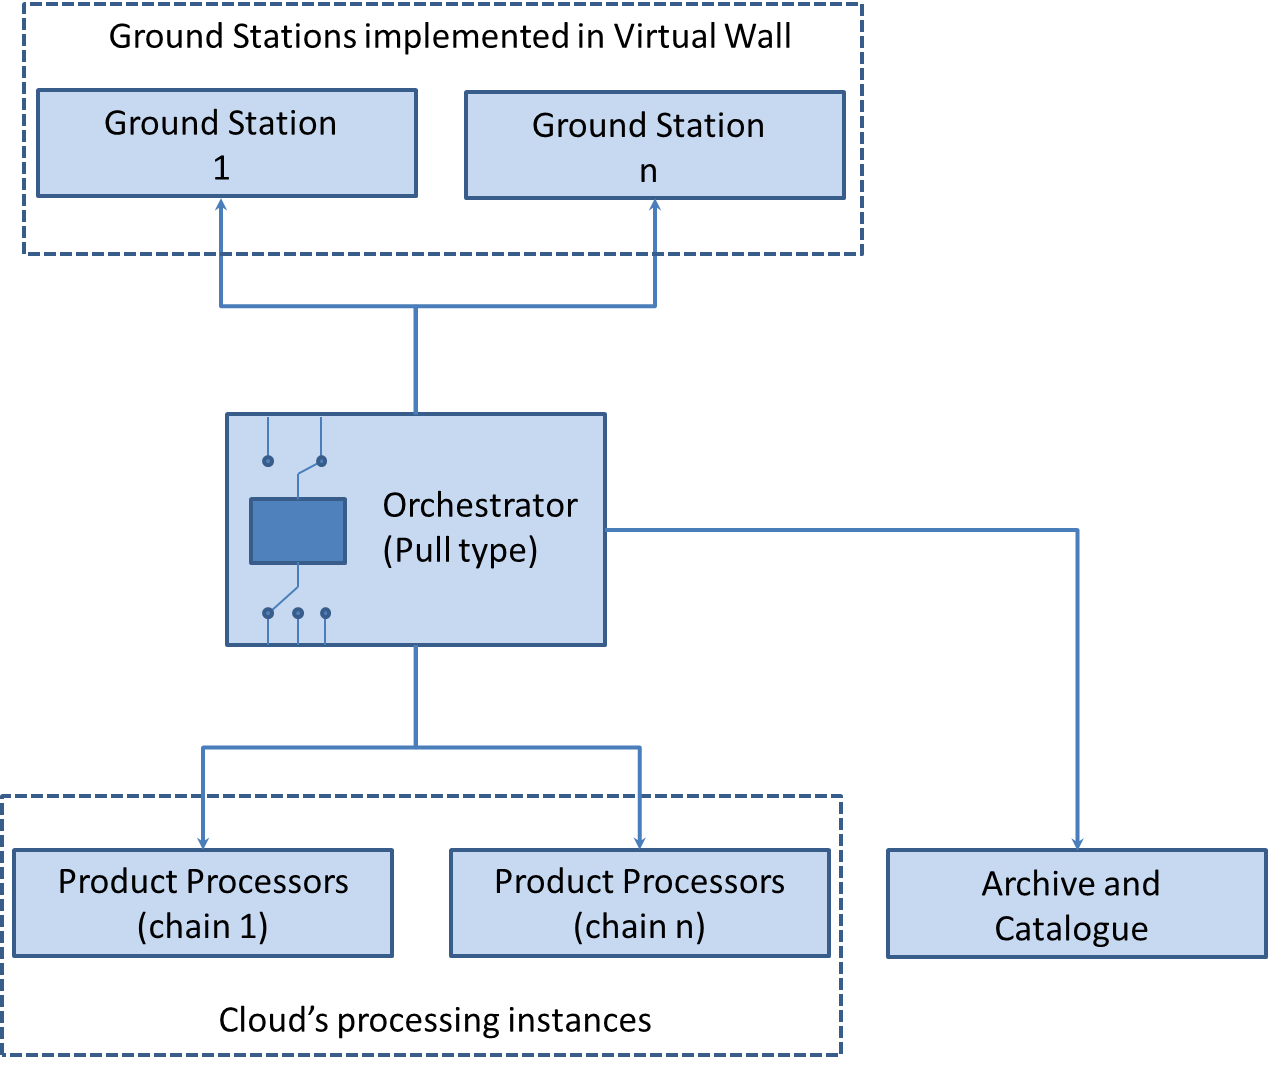
\includegraphics[width=0.7\textwidth]{cloud/orchestrator-interactions.png}
\caption{\emph{Orchestrator} interactions.}
\label{fig:orchestrator-interactions}
\end{center}
\end{figure}


As shown in Figure~\ref{fig:orchestrator-interactions}, the \emph{Orchestrator} is
pooling the Ground Stations frequently. When the \emph{Orchestrator} gets the data,
it uses the Product Processor for processing the data to generate the resulting
image. When this processing is finished, the \emph{Orchestrator} sends the image to
the \emph{Archive and Catalogue} to be available for customers.



\subsubsection{Processing Chain}
\label{subsub:processors}

The \emph{Processing Chain} is a module which is in charge of the processing of the
payload raw data from the satellites to produce image products. The four most
important operations that the product processors perform on the input data are
the following:
\begin{itemize}
\item A calibration, to convert the pixel elements from instrument digital counts into radiance units.
\item A geometric correction, to eliminate distortions due to misalignments of the sensors in the focal plane geometry.
\item A geolocation, to compute the geodetic coordinates of the input pixels.
\item An ortho-rectification, to produce ortho-photos with vertical projection, free of distortions.
\end{itemize}

The previous steps also generate quality-related figures of merit that are made
available in all the products. Moreover, the product processors generate
metadata, in line with industry standards, to facilitate the cataloguing,
filtering and browsing of the product image collection. These processors are
considerated as black boxes because they are owned by Elecnor Deimos and their
design and implementation can not be published, but them were studied for
carrying out this project.

The output image products are classified into four different levels, according to the degree of processing that they have been subjected to (see Figure~\ref{fig:cloud-states-pp}):
\begin{itemize}

\item \emph{Level 0} products are unprocessed images, in digital count numbers.
\item \emph{Level L1A} products are calibrated products, in units of radiance.
\item \emph{Level L1B} products are calibrated and geometrically corrected products (ortho-rectified), blindly geolocated.
\item \emph{Level L1C} products are calibrated and geometrically corrected products (ortho-rectified), precisely geolocated using ground control points.
\end{itemize}

\begin{figure}[!h]
\begin{center}
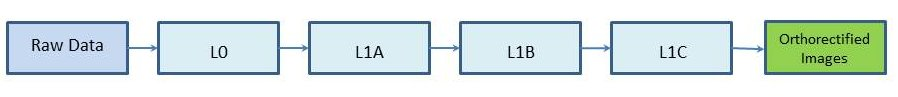
\includegraphics[width=0.9\textwidth]{detaildesign/stages-pp.jpg}
\caption{Stages of the product processing.}
\label{fig:cloud-states-pp}
\end{center}
\end{figure}

\paragraph{The L0 Processor}~\\

The acquired data is organized into image sectors of predefined size and structure and converted in scenes. Scenes, as defined here, are used throughout the subsequent L1 levels. The size and configuration of the scene is not changed again in the processing chain, for this reason the scene definition is constant for all the L1 levels.

The inputs are the following:
\begin{itemize}
\item The Raw Data.
\item The configuration database.
\item The calibration database.
\end{itemize}
The outputs are the following:
\begin{itemize}
\item The L0 products.
\end{itemize}

\paragraph{The L1A Processor}~\\

The goal of Level 1A is to calibrate the scenes. The resulting images are given in units of radiance.
The L1A component works on the scenes that compound the L0 product, performing different transformations over pixel values to generate radiances.

The inputs to the L1A level are the following:
\begin{itemize}
\item One L0 scene.
\item The configuration database.
\item The calibration database.
\end{itemize}

The output is the following:
\begin{itemize}
\item The L1A product.
\end{itemize}

\paragraph{The L1B Processor}~\\

Level 1B implements the geolocation, resampling and packing.

The inputs to the L1B level are the following:
\begin{itemize}
\item The L1A product.
\item The configuration database.
\item The calibration database.
\end{itemize}

The outputs are the following:
\begin{itemize}
\item The L1B products.
\end{itemize}


\paragraph{The L1C Processor}~\\

The L1C processor performs the ortho-rectification of the L1B product using ground control points.

The inputs to the L1C level are the following:
\begin{itemize}
\item The L1B  product.
\item The calibration database.
\item The configuration database.
\end{itemize}

The output is the following:
\begin{itemize}
\item Orthorectified Images.
\end{itemize}




\subsubsection{Archive and Catalogue}
\label{sub:archive}

The \emph{Archive and Catalogue} is a shared space of memory between the
\emph{Orchestrator}, the product processors and the distribution of data. It has
a data acquisition component which manages the input data arriving to the
\emph{Archive and Catalogue}. The ingestion of data in this module is automatic.

In the \emph{Archive and Catalogue} module the processed images are stored and catalogued for their distribution.

The \emph{Archive and Catalogue} basically consists of the archive and the
catalogue sub-modules:
\begin{itemize}
\item The \emph{Archive} is constituted by optimized storages structure allowing managing a big amount of data, efficient storage and retrieval of any kind of file. The \emph{Archive} is organized in hierarchical levels of storage in order to provide a cost effective storage solution.

\item The \emph{Catalogue} stores an inventory database with the metadata of archive files. It allows the product process chain easiness to access to the metadata from the processed products.

\item For the added value services the catalog will be accessed by a \emph{Web Service}.

\item \ac{CSW} is a module with the \ac{CSW} standard for the catalogue (based on \ac{OGC} standard). For more information on \ac{CSW}, please refer to \ac{OGC} \emph{OpenGIS Implementation Specification 07-006r1} and the \ac{OGC} tutorial on \ac{CSW}. Through this standard the distribution of data is done.
\end{itemize}

\begin{figure}[!h]
\begin{center}
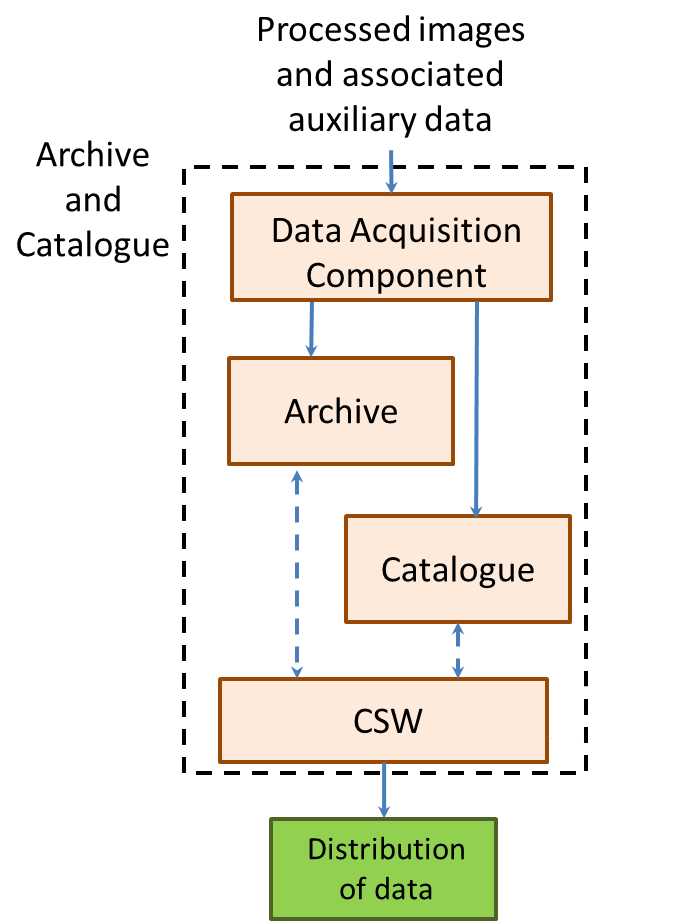
\includegraphics[width=0.5\textwidth]{detaildesign/scheme-archive-catalogue1.png}
\caption{Scheme of the \emph{Archive and Catalogue} module.}
\label{fig:archive-catalogue-scheme}
\end{center}
\end{figure}



\subsection{Implementation of the cloud architecture using SSH and SCP}
\label{subsec:ssh-cloud}
The cloud implementation using \ac{SSH} and \ac{SCP} is based in the following
components:
\begin{itemize}
\item The \emph{Orchestrator} module.
\item The \emph{Processing Chain} module.
\item The \emph{Archive and Catalogue} module.
\end{itemize}

The diagram in Figure~\ref{fig:first-architecture} shows the entire architecture is shown. The
communications were done using \ac{SSH} commands and the sending of the files were
performed using the \ac{SCP} protocol. For this implementation the raw data
travels from the \emph{Orchestrator} to the \emph{Processing Chain} module, where it is
processed. 
Finally, the Proccesing Chain module sends the processed image to the
Archive and
Catalogue module. 

It is important to highlight that the
\emph{Orchestrator} does not send the processed image to the \emph{Archive and Catalogue}
module, the \emph{Processing Chain} module sends it for archiving and cataloguing. Consecuently, the time for
archiving and cataloguing for each processed image was reduced.

\begin{figure}[!h]
\begin{center}
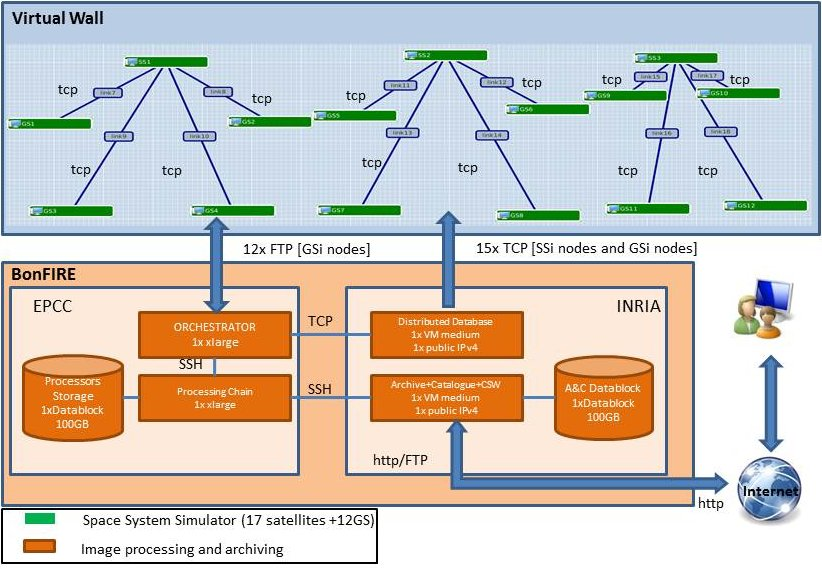
\includegraphics[width=1.0\textwidth]{cloud/first-architecture.jpg}
\caption{First architecture on cloud.}
\label{fig:first-architecture}
\end{center}
\end{figure}

The different components which compound the cloud architecture are fully
explained in the following sections. For each component, the  workflow, the
design, the implementation of the component and how was implemented in \bonfire are detailed.

\subsubsection{Implementation of the Orchestrator}

\paragraph{Orchestrator Workflow}~\\

The \emph{Orchestrator} component works by following the next sequence of steps:
\begin{enumerate}
\item The \emph{LoadData object} gets all the information about the \emph{Ground
    Stations Simulators} and localizes them.
\item The \emph{Listener object} pools to the \emph{Ground Stations} and when there are
  a downloadable raw data, the \emph{New\_Data\_Event} is launched.
\item  When the \emph{New\_Data\_Event} occurs, the \emph{Orchestrator} downloads the data.
\item  The \emph{Orchestrator} moves the raw data to a shared storage.
\item Then, the \emph{Orchestrator} makes different \emph{Job Orders} for the processors. The \emph{Job Order} contains all the useful information for the \emph{Product Processors} to proceed with the image processing.
\item The \emph{Orchestrator} gets the \emph{ProcessorChainController} object (this object was made regarding \emph{Singleton pattern}).
\item The \emph{Orchestrator} instructs the \emph{ProcessorChainController}
  object to create a new processing chain by sending the \emph{JobOrders}
  created in step 4. If there were any image processing, the request is queued.
\item The \emph{ProcessorChain Controller} object creates a new \emph{Processing
  Chain} to remotely process the data.
\item The \emph{Processing Chain} sequentially executes the L0, L1A, L1B, L1C processors.
\item When the \emph{ProcessingChain} has finished, this notifies the \emph{ProcessorChainController} object that the processing ended.
\item The \emph{ProcessingChainController} alerts the \emph{Orchestrator} that the \emph{Processing Chain} has finished.
\item The \emph{Orchestrator} takes the created image and puts it into the
  \emph{Archive}. As a improvement, this communication was not done. The
  sending to archiving and cataloguing is performed when the \emph{Processing Chain}
  finishes and sends the image to \emph{Archive and Catalogue} module. 
\end{enumerate}

Figure~\ref{fig:orchestrator-workflow} depicts the workflow of the \emph{Orchestrator}.

\begin{figure}[!h]
\begin{center}
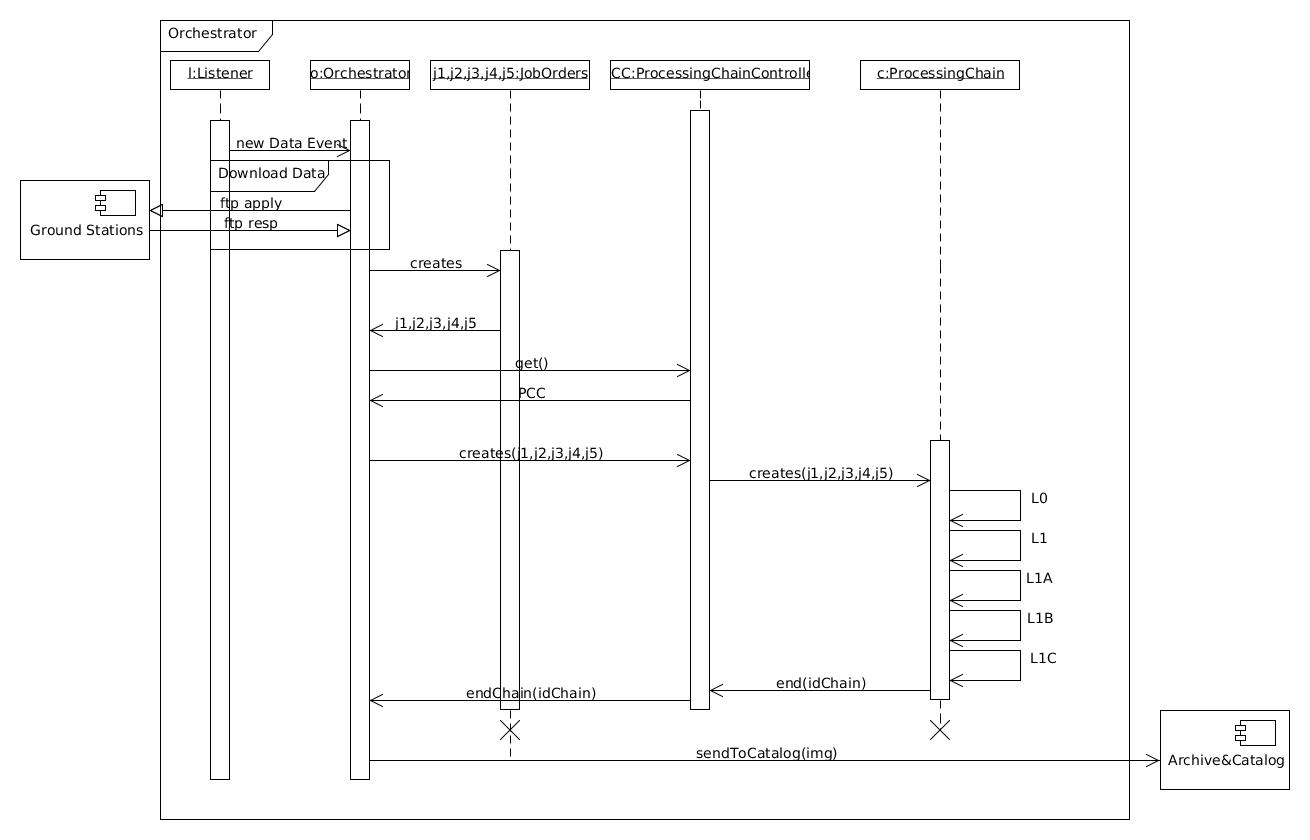
\includegraphics[width=1.0\textwidth]{cloud/orchestrator-workflow.jpg}
\caption{\emph{Orchestrator} workflow.}
\label{fig:orchestrator-workflow}
\end{center}
\end{figure}

\paragraph{Orchestrator Interfaces}~\\

The \emph{Orchestrator} has interfaces with the Ground Stations implemented in
\emph{Virtual Wall}, with the \emph{Product Processors} and with the
\emph{Archive and Catalogue}.
\subparagraph{Interfaces with the Ground Stations implemented in Virtual
  Wall}~\\

The \emph{Ground Stations} are deployed in some \emph{Virtual Wall} nodes. There, the impairments and features of the network are simulated. Essentially,
the \emph{Orchestrator} is pooling those \emph{Ground Stations} over \ac{FTP}
connections to know when new raw data is available. So, this Ground Stations are
\ac{FTP} servers in which the \emph{Orchestrator} can get the raw data obtained
by the constellation of satellites.

\subparagraph{Interfaces with the Product Processors}~\\

The \emph{Orchestrator} communicates with the \emph{Product Processors} through
the \emph{ProcessingChainController} instance as shown in
Figure~\ref{fig:orchestrator-workflow}. The \emph{Orchestrator} commands via
\ac{SSH} the \emph{ProcessingChainController} to create a new processing chains
to process the raw data and sends it through an \ac{SCP} transmission. \\
When this
process finishes, the \emph{ProcessingChainController} sends  a message to
indicate the end of the chain to the \emph{Orchestrator}. Thus, the
\emph{ProcessingChainController} checks the product processors progress and
initiates the next level until the processing chain finishes. Finally, the
\emph{Processing Chain} obtains the end product and locates it in the Catalogue service. 

\paragraph{Orchestrator Design}~\\

The Orchestrator is formed by the \emph{Listener}, the \emph{JobOrder} and
the \emph{ProcessingChainController}, the \emph{Orchestrator} and the \emph{Load} classes.

\begin{itemize}
\item \emph{Listener class}: It is responsible of obtaining the \emph{FTP}
  connections and polling them in order to get the images when they are created in the
  ground stations. When an image is detected in any ground station, a thread is
  created to download it. Then, the \emph{Orchestrator} object is signaled in order
  to begin the processing.
\item \emph{JobOrder class}: It perform the creation of the job orders. For
  simplicity, a specific job order is always used in all
  processings of scenarios.
\item \emph{ProcessingChainController class}: It  manages the processing in the
  product processors via \ac{SSH}. The processing is remotely executed. When an image is
  sent by the \emph{Orchestrator} class to the ProcessingChainController class, a
  new thread is created. Then, this thread remotely processes the image in the
  ProcessingChain module. If any request comes at same time, it is queued.
  This is a class based in the Singleton pattern.
\item \emph{Orchestrator class}: This class is designed by following a \emph{Controller}
  pattern. It manages the interactions between all above classes and integrates
  them.
\item \emph{LoadData class}: it parsers the configuration file for obtaining the
  \ac{IP} addresses of Database node, \emph{Archive and Catalogue} node and the
  \emph{Processing Chain} module. Furthermore, the user and password for \ac{FTP}
  connections are included into the configuration file. 
\end{itemize}



\paragraph{Orchestrator Implementation}~\\

The implementation of this module was done in Python 2.7. The libraries
needed to implement the software are listed in Table~\ref{table:orches-first-libraries}.

\begin{table}[hp]
  \centering
  {\small
  


\begin{tabular}{p{.2\textwidth}p{.2\textwidth}}
  \tabheadformat
  \tabhead{Python Library}   &
  \tabhead{Function}\\
\hline
\textit{Threading}         & System library for creating ,syncronizing and managing threads \\
\hline
\textit{OS}         & Library which provides operative system interactions \\
\hline
\textit{Collections}         & Library that contains the data structure
``deque'' used for queueing the request which can not be processed.\\
\hline
\textit{Time}         & For managing the time \\
\hline
\textit{Socket}         & Library for creating and establishing connections with other host \\
\hline
\textit{Pdb}         &  Used for debugging the software\\
\hline
\textit{FtpLib}         &Library used to obtain and manage the Ground Stations' FTP connections  \\
\hline
\end{tabular}


% Local variables:
%   coding: utf-8
%   ispell-local-dictionary: "castellano8"
%   TeX-master: "main.tex"
% End:

  }
  \caption{Orchestrator’s Python Libraries.}
  \label{table:orches-first-libraries}
\end{table}

Moreover, it requires the \ac{SCP} and \ac{SSH} clients for communicating  with other
modules in the cloud.
In addition, a script was developed in order to obtain the workload of the
\emph{Orchestrator} machine. That file uses the ``Python-psutil'' library in order to
obtain the CPU times such as user, idle, nice and iowait cycles. This file is
used by the graphical interface for plotting the workload of the \emph{Orchestrator} at
real time.


\paragraph{Orchestrator Execution}~\\

To execute the \emph{Orchestrator} module the following dependencies are required:
\begin{itemize}
\item Python v.2.7. For previous versions it has not been tested.
\item Python packages listed in Table~\ref{table:orches-first-libraries}.
\item Ethernet interface for the network connection in the \bonfire \emph{WAN}.
\item Connectivity with the database located in \bonfire through the network.
\item To setup the ``orchestrator.conf.xml'' with the correct \ac{IP} addresses
  of \emph{Archive and Catalogue} node, Chain Processing node and database node.
\end{itemize}

The execution of the satellite software it is executed inside the
``source/bonfire/orchestrator'' with the following
command line:
\begin{itemize}
\item[>] python main.py
\end{itemize}
 
\paragraph{Implementation in BonFIRE}~\\

For implementing of the \emph{Orchestrator} the following steps were done:

\begin{itemize}
 \item Reservation of a \emph{Xlarge} machine in \emph{EPCC} \bonfire
   platform. This machine belongs the \bonfire \emph{WAN} so it can communicate
   with all machines in that network. 
 \item Instalation of the necessary libraries (see
   Table~\ref{table:orches-first-libraries}).
 \item To upload the \emph{Orchestrator}' source to the \emph{Orchestrator} machine.
 \item To generate a pair of \ac{RSA} keys for enabling the connections to
   \emph{Procesing Chain} node.
\end{itemize}

\subsubsection{Implementation of the Processing Chain}

The implementation of the \emph{Processing Chain} was performed in a bash script. This script is remotely executed by the \emph{Orchestrator} for processing the
images. It was made in this manner because this is an implementation for testing the
processing behaviour on cloud. The elastic service provided by the \bonfire
platform was not available, so as a first approach, a machine was fixed for
testing the architecture.\\
 Furthermore, the clustering service provided for
\emph{INRIA} did not also work, so the dinamic creation of processes can not be
done because a only processing chain needs as minimum 6 GB of RAM memory. At the
end, only a Chain Processing at time can be executed, so this implementation is
very restricted in performance. 

\paragraph{Processing Chain Workflow}~\\

The \emph{Processing Chain} component works by following the next sequence of
steps:

\begin{enumerate}
\item The \emph{Orchestrator} component sends the image using \ac{SCP} to the
  directory ``tmp'' in the \emph{Processing Chain} machine.
\item The \emph{Orchestrator} remotely executes the script ``PP\_script.sh''
  located in the \emph{Processing Chain} machine.
\item The image processing start. The processors are sequentially executed.
\item When all the product processors have finished, the \emph{Processing Chain}
  sends the orthorectified image to \emph{Archive and Catalogue} using
  \ac{SCP}. 
\item The \emph{Processing Chain} orders the \emph{Archive and Catalogue} module
 to archive and catalogue the image received. In the first development, the
 \emph{Processing Chain} returned the results to the \emph{Orchestrator} and the
 orchestrator sent the images to the \emph{Archive and Catalogue} module for cataloguing
 and archiving. But that implementation was inefficient because there were two
 sending files more (the first one is between the \emph{Processing Chain} to the
 \emph{Orchestrator} and the second one, between the \emph{Orchestrator} and
 \emph{Archive and Catalogue}. Finally, the solution was to
 accomplish only a sending. The \emph{Processing Chain} after processing sends
 the results for archiving and cataloguing. 
\end{enumerate}

\paragraph{Processing Chain Interfaces}~\\

The \emph{Processing Chain} module has interfaces with both the \emph{Orchestrator}
and the \emph{Archive and Catalogue} modules.
\subparagraph{Interfaces with the Orchestrator}~\\

The \emph{Orchestrator} communicates with the \emph{Processing Chain} for
processing new incoming raw data. This communication is carried out using \ac{SCP} for file sending and for remote commands, (\ac{SSH}). This provides a manner of creating processes
on-demand. If the \emph{Processing Chain} machine was running in a cluster or
under an \ac{EaaS}, the
resources would be dinamically requested. 

\subparagraph{Interfaces with the Archive and Catalogue}~\\

The \emph{Archive and Catalogue} receives the images which the \emph{Processing
  Chain} has processed. The transfer of the images is performed using \ac{SCP}. Then, the
\emph{Processing Chain} remotely executes a Python script in the \emph{Archive
  and Catalogue} machine for archiving and
cataloguing the sent image.

\paragraph{Processing Chain Design}~\\

The \emph{Processing Chain} is formed by the ``PP\_script.sh'' bash
script. Originally, this module will be located in an \emph{EaaS}. The \bonfire
platform has not available this feature yet, so it was decided to push into a
cluster provided by the \emph{INRIA} testbed. The cluster platform was not also
available, so it was necessary to create and fix a machine which plays the
\emph{Processing Chain} role with the restriction that there can only be one
instance. 

\paragraph{Processing Chain Implementation}~\\
\label{par:pp-impl}
The implementation of this module was done using a bash script. This script needs the
\ac{IP} address of the \emph{Archive and Catalogue} module. In addition, it
requires the \ac{SCP} and \ac{SSH} clients for its interfaces with the other
modules. The image which is sent to the \emph{Archive and Catalogue} when the
process is finished, it is always the
same because for the experiment is more important the processing on cloud than
the resulting image.
  
In addition, a script was developed in order to obtain the workload of the
\emph{Orchestrator} machine. That file uses the ``Python-psutil'' library in order to
obtain the CPU times such as user, idle, nice and iowait cycles. This file is
used by the graphical user interface for plotting the workload of the \emph{Orchestrator} at
real time.

Finally,  shared storage was used to store the images instead of
the local storage. The shared storage is provided by the \emph{IBBT} testbed. This storage is implemented using \ac{NFS} protocol. Ideally, the \ac{NFS}
protocol using a network with a large bandwidth and links with 10 GB Ethernet is
more efficient than using a local hard disk. However the \ac{NFS}
server is not conformed by disks located in the \bonfire platform. The physical disks
where the information is saved are in \emph{IBBT} located in Ghent (Belgium). Thus, the
read and write accesses from any \bonfire testbed (INRIA and EPCC in this case)
travel from \bonfire to \emph{IBBT} through the Internet. This involves high
latencies, large waiting times and it implies that the CPU is idle large time
waiting for I/O operations. These results are shown in Section~\ref{sec:geocloud-results}.

The implementation of this shared storage was performed as follows:
\begin{itemize}
\item In the \bonfire web interface, a shared storage was created. 
\item The folders structure for processing were done. This structure is composed
  by (the local structure has the same distribution): 
\begin{itemize}
\item Job orders folder: it contains the job orders necessary for processing all
  stages.
\item l0\_input folder: it contains the neccesary inputs for L0 processor. 
\item l0r\_input folder: it contains the neccesary inputs for L0R processor. 
\item l1a\_input folder: it contains the neccesary inputs for L1A processor. 
\item l1br\_input folder: it contains the neccesary inputs for L1BR processor. 
\item l1bc\_input folder: it contains the neccesary inputs for L1BC processor. 
\item l1cr\_input folder: it contains the neccesary inputs for L1CR processor. 
\item l1ct\_input folder: it contains the neccesary inputs for L1CT processor. 
\end{itemize}
\item Processors outputs folder: contains the outputs and temporaly files
  created by the processors during their actions.
\end{itemize}

\paragraph{Processing Chain Execution}~\\

To execute the \emph{Processing Chain} module the following dependencies are
required:
\begin{itemize}
\item To know the \ac{IP} address of the \emph{Archive and Catalogue}.
\item Ethernet interface for the network connection in the \bonfire \emph{WAN}.
\item The geolocated image for sending to \emph{Archive and Catalogue} module
  once the processing is finished. 
\item The Product Processors owned by \emph{Elecnor Deimos} installed in the
  machine.
\end{itemize}

The script is located inside
``source/bonfire/ProcessingChain'' folder. The execution of the software is executed with the following
command line:
\begin{itemize}
\item[>] bash PPscript.sh <<arg1>> <<arg2>>
\end{itemize}
where \emph{arg1} is the outfile name in which the \emph{Archive and Catalogue} module
saves the image and the \emph{arg2} is the simulated scenario.


\paragraph{Implementation in BonFIRE}~\\

To implement the \emph{Processing Chain} module the following steps were done:

\begin{itemize}
 \item Reservation of a \emph{Xlarge} machine in \emph{EPCC} \bonfire
   platform. This machine belongs the \bonfire \emph{WAN} so it can communicate
   with all the machines in that network. 
 \item Installation of the product processors.
 \item Uploading the geolocated image.
 \item Uploading the \emph{ProcessingChain} source to the \emph{ProcessingChain}
   machine.
 \item Appending the public key from \emph{Processing Chain} machine to the
   \emph{``~/.ssh/authorized\_host''} to allow the incoming connections.
\end{itemize}

\subsubsection{Archive and Catalogue}

The first implementation of the \emph{Archive and Catalogue} component was
performed for archiving and cataloguing the geolocated images which were
processed in the simulation of the defined scenarios. It is based on the
\emph{GeoServer} software. The inputs are given by the \emph {Processing Chain}
module when it finishes the processing of an image. It sends the image using
\ac{SCP} and then, it remotely executes the Python script for archiving and
cataloguing the image. Once the image is catalogued, the end user can access it
with the \emph{IP} address of the node using a web-browser. Then
\emph{GeoServer} is showed and the end user can navigate between the different
scenarios and files generated in the execution of the experiment.

\paragraph{Archive and Catalogue Workflow}~\\

The \emph{Archive and Catalogue} component works by following the next sequence
of steps:
\begin{enumerate}
\item The \emph{Processing Chain} ends its processing and sends the resulting
  image via \ac{SCP} to the \emph{Archive and Catalogue} 
\item The Python script is remotely executed by the \emph{Processing Chain}
  by using \ac{SSH}.
\item The script obtains the image for archiving and copies it into the
  \emph{GeoServer} data directory.
\item The image is catalogued by using the \ac{API} provided by
  \emph{GeoServer}. If the scenario was not created as a workspace, the
  workspace is created.
  \item A store is created in order to house the image.
  \item The image is catalogued in the workspace and stored in the created store.
  \item The \emph{GeoServer} module publishes the catalogued image using the
  \ac{CSW} protocol. Any end user connectig the web interface can access the
  catalogued and published images of the scenarios.
\end{enumerate}

\paragraph{Archive and Catalogue Interfaces}~\\

The \emph{Archive and Catalogue} has interfaces with the \emph{Processing Chain}
and the \emph{GeoServer} software. 

\subparagraph{Interfaces with the Processing Chain}~\\

When the \emph{Processing Chain} module has finished the processing of an image,
it sends the image to the \emph{Archive and Catalogue} module via \ac{SCP} protocol to proceed with its archive and catalogue. The
\emph{Archive and Catalogue} recives the image and stores it into the data
directory of \emph{GeoServer}. Then, the \emph{Processing Chain} remotely orders
to catalogue this image.  

\subparagraph{Interfaces with the GeoServer software}~\\

The \emph{GeoServer} software provides a Python library namely
\emph{Gsconfig}. The official page of this library is
\url{https://github.com/boundlessgeo/gsconfig}. Using this library, operations
with layers, images, tilesets or storages can be done. The provided operations
for cataloguing ``tiff'' images (the default format for geodata images) were used in this project.

\subparagraph{Interfaces with CSW clients}~\\

The \emph{GeoServer} software implements a \ac{CSW} plugin to provide the end users
a \ac{CSW} interface instead of a web-browser for accesing the catalogue.
This feature provides a new connectivity channel for data interchange between
modules of others projects, business or end users.

\paragraph{Archive and Catalogue Design}~\\

The \emph{Archive and Catalogue} is formed by the \emph{GeoServer} software and
a Python script for communicating with \emph{GeoServer} in order to catalogue
and store the processed images.

The script communicates with the \emph{GeoServer} software for creating a
workspace, for creating data stores and for cataloguing the images were sended
by the \emph{Processing Chain}. 


incluir esquema script -> geoserver -> csw o http

\paragraph{Archive and Catalogue Implementation}~\\

The implementation of this module was done in Python 2.7. The python's libraries
needed to implement the software are listed in
Table~\ref{table:ayc-first-libraries}.

\begin{table}[hp]
  \centering
  {\small
  


\begin{tabular}{p{.2\textwidth}p{.2\textwidth}}
  \tabheadformat
  \tabhead{Python Library}   &
  \tabhead{Function}\\
\hline
\textit{Time}         & For managing the time \\
\hline
\textit{Pdb}         &  Used for debugging the software\\
\hline
\textit{Gsconfig}         &Library used to communicates with \emph{GeoServer} software \\
\hline
\textit{OS}         & Library which provides operative system interactions \\
\hline
\textit{Sys}         & System library \\
\hline
\end{tabular}


% Local variables:
%   coding: utf-8
%   ispell-local-dictionary: "castellano8"
%   TeX-master: "main.tex"
% End:

  }
  \caption{ICE Archive and Catalogue Python Libraries.}
  \label{table:ayc-first-libraries}
\end{table}

The \emph{Gsconfig} library was manually installed as follows:
\begin{itemize}
\item The library obtained from the following url: \url{https://github.com/boundlessgeo/gsconfig}.
\item Firstly, the ``Python-pip''  package is installed.
\item Then just execute ``pip install gsconfig''.
\end{itemize}

Then, the \emph{GeoServer} software was required to be installed. For that purpose, the
\emph{Apache Tomcat} server was installed. Then, the ``war''
file which contains the \emph{GeoServer} software was downloaded from the official webpage and
it was installed into the \emph{Tomcat} server. In Section~\ref{para:bonfire-impl-cat} this process
is explained in detail. 

\paragraph{Archive and Catalogue Execution}~\\

To execute the \emph{Archive and Catalogue} module the following dependencies
are required:
\begin{itemize}
\item \emph{Apache Tomcat}
\item \emph{Geoserver with the \ac{CSW} plugin}
\item \emph{Gsconfig library installed}
\item \emph Ethernet interface for the network connection in the \bonfire
  \emph{WAN}.
\item \emph Ethernet interface for the network connection with a public \ac{IP}
  address. In this project an \ac{IP}v4 was used.
\end{itemize}

The developed source for archiving and cataloguing is located in
``source/bonfire/geoserver''. The execution of the \emph{Archive and Catalogue}
module namely ``catalog\_pp.py'' is done as follows:
\begin{itemize}
\item[>] python catalog\_pp.py <<name\_file>> <<scenario>> <<nameStore>>
\end{itemize}
where <<name\_file>> is the absolute path of the image to the \emph{Archive and Catalogue},
<<scenario>> is the scenario in which the image is catalogued and the
<<nameStore>> is the name of the created store for housing the image.

\paragraph{Implementation in BonFIRE}~\\
\label{para:bonfire-impl-cat}


For implementing the \emph{Archive and Catalogue} module the following steps were done:

\begin{itemize}
 \item Reservation of a \emph{Medium} machine in \emph{INRIA} \bonfire
   platform. This machine belongs to the \bonfire \emph{WAN} so it can communicate
   with all the machines in that network. Moreover it has a public \ac{IP} address
   in order to be accesible outside the \bonfire network by end users. 
 \item Installation of the Java version 6.
 \item Installation of the \emph{Apache Tomcat} server and its customization in
   order to listen in port 80 and to reserve the necessary requirements for Java.
 \item Installation of the \emph{GeoServer} and the \emph{CSW} plugin in
   \emph{Apache Tomcat}. In the CD-ROM attached the setup script for this step
   is included.
 \item Uploading of the geolocated image.
 \item Uploading of the \emph{ProcessingChain} source to the \emph{ProcessingChain}
   machine.
 \item Appending the public key from \emph{Processing Chain} machine to the
   \emph{``~/.ssh/authorized\_host''} for
   allowing the incoming connections.
\end{itemize}


\subsection{Implementation of the cloud architecture using ZeroC ICE}

ZeroC ICE provides multiple services to create distributed
architectures. By using its replication service, load balancing and location
transparency the following architecture can be obtained.
The components of the architecture implemented with ZeroC ICE and their
interrelations are represented in Figure~\ref{fig:ice-architecture}. The layers
of the cloud architecture are the
following:
\begin{itemize}
\item Layer 1: the ZeroC ICE distributed platform. It provides the runtime environment
  where distributed components can be deployed conforming a distributed
  architecture.
\item Layer 2: the cloud architecture. It defines the logical nodes in which the
  servers (components of the system) are deployed.
\begin{itemize}
\item \emph{Orchestrator} node: it is the node in which the \emph{Orchestrator} server
  is deployed.
\item \emph{Broker node}: it is the node in which the \emph{Broker} server is
  deployed.
\item \emph{Processing Chain node}: it is the node in which the \emph{Processing
  Chain} server is deployed.
\item \emph{Archive and Catalogue} node: it is the node in which the
  \emph{Archive and Catalogue} is deployed.
\end{itemize}
\item Layer 3: the architecture servers (also namely component). It defines the basics features such
  as their relations and interfaces that the components require. In this architecture, the following servers were defined:
\begin{itemize}
\item \emph{Client/Ground Stations}: it is the client of the architecture but it
  is not included in it. This component is used by the experimenter to
  initialize the experiment. Moreover, in the client attached in the CD-ROM, it
  also says to the \emph{Orchestrator} that new raw data is available. In this
  project the client implementation was done to check the funcionality of the
  architecture. The implementation of the client
  funcionality in the Ground Stations implemented in \vw may be future work.
\item \emph{Broker} server: it acts as an intermediary between the client and the cloud architecture
  components. 
\item \emph{Orchestrator} server: this component manages the ingestion and the
  processing the raw data and archiving and cataloguing the images obtained. It was explained in Section~\ref{sub:orch}.
\item \emph{Processing Chain} server: this component proccesses the images downloaded by the
  \emph{Orchestrator} module and it notifies the \emph{Orchestrator} when it
  finishes. All \emph{Processing Chains} servers are joined into a Replica Group namely
  \emph{ProcessingChainReplica module}. It provides the replication service and the load
  balancing. When it receives a request for processing, it selects one of the 
  \emph{Processing Chain} servers which less workload has.
\item \emph{Archive and Catalogue} server: it archives and catalogues the images. It was explained in Section~\ref{sub:archive}.
\end{itemize}
\end{itemize}
\begin{figure}[!h]
\begin{center}
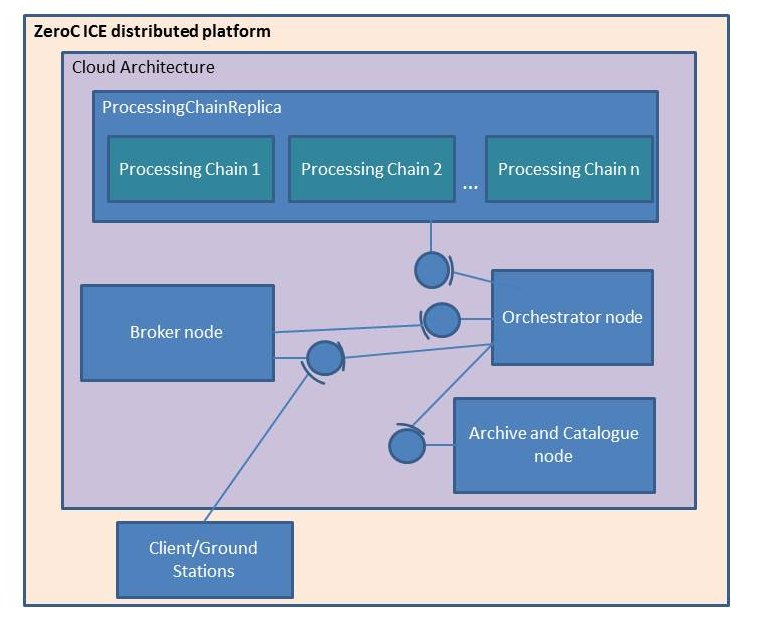
\includegraphics[width=0.95\textwidth]{cloud/second-architecture.jpg}
\caption{Cloud architecture using ZeroC ICE.}
\label{fig:ice-architecture}
\end{center}
\end{figure}


This architecture is independent of the platform when it is executed. There are
logical nodes in which ICE deploys the servers. These nodes may match with
physical nodes or may be several logical nodes in the same physical node. The
ICE runtime manages the location of the servers and their execution.

Furthermore, the data store is shared between all the servers. This means that the
components such as the \emph{Orchestrator}, the \emph{Archive and Catalogue} and the
\emph{Processing Chains} share the same logical memory space and they can write or read data
at the same time. This implementation avoids the file transfers and it does the
cloud infrastructure clearer, more dynamic and scalable.

In the following sections the  ICE interfaces between these components are
shown and the previous modules modules are explained. Their design and
interfaces with other modules are described. Finally, the
deployment of the software in each module is explained in detail.

\subsubsection{ICE interfaces}

The distributed application using ZeroC ICE was made using a slice file namely
``Geocloud.ice''for
specifying the  interfaces between components. These interfaces allows the transparently
communication between the components. The slice file is listed in Listing~\ref{code:ice-slice}.


\begin{listing}[
  float=h!,
  caption  = {Slice of the ICE application.},
  label    = code:ice-slice,
style=customc]

module geocloud {
    exception AlreadyExists { string key; };
    exception NoSuchKey { string key; };
    exception CreationScenarioException{};
    exception StartScenarioException{};
    exception StopScenarioException{};
    exception DeleteScenarioException{};
    exception ArchiveNotAvailableException{};
    exception OrchestratorNotAvailableException{};
    exception ProcessingException{};
    exception CataloguingException{};

    interface Orchestrator{
    	void initScenario(int scen) throws StartScenarioException,ArchiveNotAvailableException;
	void downloadedImage(string path);//the ground station calls this operation passing the path
	void imageProcessed(string path);
	void imageCatalogued(string path);
	void stopScenario() throws StopScenarioException;
    };

    interface Broker{
	void startScenario(int scen) throws OrchestratorNotAvailableException, StartScenarioException;
	void appendLog(string newLog);
	void stopScenario(int scen);
	void setOrchestrator( Orchestrator * orch);
	string getLastLogs();
    };


 interface Processor{
	//int init( Broker * log);
       	void processImage(string path) throws ProcessingException;
	void shutdown();
	void setOrchestrator(Orchestrator * orch);
    };



    interface ArchiveAndCatalogue{
	void createScenario(string scenario) throws CreationScenarioException;
	void catalogue(string path,string storage,string scenario) throws CataloguingException;
	void deleteScenario(int scenario) throws DeleteScenarioException;
    };
};
\end{listing}

\subsubsection{Implementation of the Orchestrator}

The \emph{Orchestrator} performs the same task that in the architecture based in
\ac{SSH} and \ac{SCP} (see Section~\ref{subsec:ssh-cloud}). It connects with the ground stations over \ac{FTP} connections and
then, the communications between the components of the cloud are done by using the
ICE interfaces of each component. ICE uses \ac{TCP} protocol by default.

\paragraph{Orchestrator Workflow}~\\

The \emph{Orchestrator} component works by following the next sequence of steps:
\begin{enumerate}
\item The ICE core application is initialized and the ICE communicator is
  created.
\item The \emph{Orchestrator Object Adapter} is instantiated and the \emph{Orchestrator} servant is
  added to it.
\item In the \emph{Orchestrator} initialization, the \emph{Listener} process is spawned.
\item The \emph{Listener} process creates the \emph{LoadData} object for loading the ground
  stations \ac{IP} addresses and the \ac{FTP} credentials.
\item The \emph{LoadData object} gets all the information about the \emph{Ground
    Stations Simulators} and localizes them.
\item The \emph{Listener} pools the \emph{Ground Stations} and when there are
  a downloadable raw data, the Orchestrator's function \emph{donwloadedImage} is
  called passing the absolute path of the image as parameter. 
\item  When the \emph{downloadedImage} is called, the \emph{Orchestrator}
  obtains the data.
\item  The \emph{Orchestrator} moves the raw data to a shared storage.
\item Then, the \emph{Orchestrator} makes different \emph{Job Orders} for the Processing Chains. The \emph{Job Order} contains all the required information by the \emph{Product Processing Chains} to proceed with the image processing.
\item The \emph{Orchestrator} gets the \emph{ProcessorChainReplica} proxy (this
  replica group contains all the Processing Chains in the cloud) and calls the
  \emph{processImage} operation of the proxy.
\item When the selected \emph{Processing Chain} finishes, it calls the \emph{processedImage}
  operation of the \emph{Orchestrator}.
\item The \emph{Orchestrator} obtains the \emph{Archive and Catalogue} proxy and
  sends the absolute path of the image for archiving and cataloguing.
\end{enumerate}

\paragraph{Orchestrator Interfaces}~\\

The \emph{Orchestrator} has interfaces with the Ground Stations implemented in
\emph{Virtual Wall}. Moreover this component  communicates with the \emph{Product Processing Chains} through the Replica
Group and with the
\emph{Archive and Catalogue}. 

\subparagraph{Interfaces with the Ground Stations implemented in Virtuall
  Wall}~\\

The \emph{Ground Stations} are deployed in some \emph{Virtual Wall} nodes. In
those, the impairments and features of the network are simulated. Essentially,
the \emph{Orchestrator} is pooling those \emph{Ground Stations} over \ac{FTP}
connections to know when new raw data is available. So, this Ground Stations are
\ac{FTP} servers in which the \emph{Orchestrator} can get the raw data recorded
by the constellation of satellites. 
As the ICE implementation could not be
deployed in the \bonfire platform, the checking and testing of funcionalities
were locally done. Thus, a client playing as a Ground Station was developed in
order to check and validate the architecture. 

\subparagraph{Interfaces with the  Processing Chains}~\\

The interfaces which the \emph{Processing Chains} provides are listed in
Listing~\ref{code:ice-slice}. The operations that the \emph{Orchestrator} uses
are \emph{processImage} and \emph{setOrchestrator} operations. 

\subparagraph{Interfaces with the Archive and Catalogue}~\\

The interfaces which the \emph{Archive and Catalogue} provides are listed in
Listing~\ref{code:ice-slice}. The operation that the \emph{Orchestrator} uses is
the \emph{catalogue} operation.


\paragraph{Orchestrator Design}~\\

The \emph{Orchestrator} module implements the \emph{Orchestrator} interface
which contains the following operations:
\begin{itemize}
\item \emph{void initScenario(int scen)}: it initializes the scenario in the
  module.
\item \emph{void downloadedImage(string path)}: it indicates to the
  \emph{Orchestrator} that an image is available to be processed  in the specified
  path.
\item \emph{void imageProcessed(string path)}: the Processing Chains call this function
  to indicate to the \emph{Orchestrator} that the processing of the image has
  finished, so the \emph{Orchestrator} can archive and catalogue it.
\item \emph{void imageCatalogued(string path)}: the catalogue module uses this
  function to notify the \emph{Orchestrator} that the image located in ``path'' was
  archived and catalogued.
\item \emph{void stopScenario(int scen)}: it stops the scenario in the
  \emph{Orchestrator}. Furthermore, it stops all the existing processing chains working.
\end{itemize}

The requests are served when they come to the \emph{Orchestrator} module. If
other request comes and the processing chains are busy, they are automatically queued by the
ICE execution core. Thus, it is not necessary to maintain a queuing algorithm in
the \emph{Orchestrator}. However it is necessary to have some data structures, in
this case dictionaries to temporaly store the images which are in different stages.

Furthermore, when the \emph{Orchestrator} is initialized the \emph{Listener} process is
accomplished. It listens the \ac{FTP} connections with the ground stations to detect and download new raw data. This process is always pooling the
ground stations until the \emph{Orchestrator} execution ends.

\paragraph{Orchestrator Implementation}~\\

The implementation of this module was done in Python 2.7 using ZeroC ICE 3.4. The
python's libraries needed to implement the software are listed in
Table~\ref{table:orches-second-libraries}

\begin{table}[hp]
  \centering
  {\small
  


\begin{tabular}{p{.2\textwidth}p{.2\textwidth}}
  \tabheadformat
  \tabhead{Python Library}   &
  \tabhead{Function}\\
\hline
\textit{Threading}         & System library for creating ,syncronizing and managing threads \\
\hline
\textit{OS}         & Library which provides operative system interactions \\
\hline
\textit{Collections}         & Library that contains the data structure
``deque'' used for queueing the request which can not be processed.\\
\hline
\textit{Time}         & For managing the time \\
\hline
\textit{Socket}         & Library for creating and establishing connections with other host \\
\hline
\textit{Pdb}         &  Used for debugging the software\\
\hline
\textit{FtpLib}         &Library used to obtain and manage the Ground Stations' FTP connections  \\
\hline
\end{tabular}


% Local variables:
%   coding: utf-8
%   ispell-local-dictionary: "castellano8"
%   TeX-master: "main.tex"
% End:

  }
  \caption{ICE \emph{Orchestrator} Python Libraries.}
  \label{table:orches-second-libraries}
\end{table}

\paragraph{OrchestratorExecution}~\\

To execute the \emph{Orchestrator} module the following dependencies
are required:
\begin{itemize}
\item \emph{ZeroC ICE 3.4} installed.
\item \emph Ethernet interface for connecting with the \emph{IceGrid} locator (see Section~\ref{subsub:deployment}).
\item \emph Configuration file for the node.
\end{itemize}
 In Section~\ref{subsub:deployment} the
  automatic deployment and execution of this module is explained. 

\subsubsection{Implementation of the  Processing Chain}

The \emph{Processing Chain} component processes the raw data to obtain a calibrated,
geolocated and orthorectified image. It executes all the product processor stages and notifies the
\emph{Orchestrator} server The background filesystem, where the cloud based in
ICE are implemented and executed, is a shared storage, so all the necessary files are
located in that shared memory space  explained in Section~\ref{par:pp-impl}. Moreover, all the instantiated \emph{Processing Chains} form part of the
\emph{ProcessingChainReplica} in order to provide load balancing and dynamic
replication services. 


\paragraph{Processing Chain Workflow}~\\

The \emph{Processing Chain} component works by following the next sequence of steps:

\begin{enumerate}
\item The \emph{setOrchestrator} operation is invoked for setting up the
  \emph{Orchestrator} in the \emph{Processing Chain}.
\item When the \emph{Orchestrator} invokes the \emph{processImage} fuction, the
  \emph{Processing Chain} starts to transform the raw data located in path.
\item When all the stages have been performed, the \emph{Processing Chain} calls the
  \emph{processedImage} of the \emph{Orchestrator}.
\item The \emph{Processing Chain} is ready for processing other image.
\item If the \emph{shutdown} function is called by the \emph{Orchestrator}, the
 \emph{Processing Chain} is turned off.
\end{enumerate}


\paragraph{Processing Chain Interfaces}~\\

The \emph{Processing Chain} component has interfaces with the \emph{Orchestrator}.

\subparagraph{Interfaces with the Orchestrator}~\\

The \emph{Processing Chain} server receives the order to process an image. When the
processing is finished, the \emph{Processing Chain} notifies the end of the
processing to the \emph{Orchestrator} by
calling the \emph{imageProcessed} function.

\paragraph{Processing Chain Design}~\\

The \emph{Processing Chain} module implements the \emph{Processor} interface, which
contains the following operations:

\begin{itemize}
\item \emph{void processImage(string path)}: it is invoked by the
  \emph{Orchestrator} in order to process the image located in path. Thus, all
  the product Processing Chains are sequentially executed and the \emph{processedImage}
  of the \emph{Orchestrator} is called. 
\item \emph{void shutdown()}: this funcion turns off the proccesor.
\item \emph{setOrchestrator()}: it sets up the \emph{Orchestrator} proxy to be
  used for the \emph{Processing Chain}.
\end{itemize}

\subparagraph{ProcessingChainReplica}~\\

This component involves all the \emph{Processing Chains} in the ICE application. It
provides two services: dynamic replication and load balancing. The first
of service is used for creating new on demand \emph{Processing Chains}. The second
one service servers the incoming petitions searching the less overloaded \emph{Processing Chain}
and returning its proxy for carrying out the request.

\paragraph{Processing Chain Implementation}~\\

The implementation of this module was done in Python 2.7 using ZeroC ICE 3.4. The
python's libraries needed to implement the software are listed in
Table~\ref{table:processor-second-libraries}.

\begin{table}[hp]
  \centering
  {\small
  


\begin{tabular}{p{.2\textwidth}p{.2\textwidth}}
  \tabheadformat
  \tabhead{Python Library}   &
  \tabhead{Function}\\
\hline
\textit{Threading}         & System library to create, syncronize and manage threads \\
\hline
\textit{OS}         & Library which provides operative system interactions \\
\hline
\textit{Pdb}         &  Used for debugging the software\\
\hline
\textit{Ice}         & ICE general purpose library \\
\hline
\textit{IceGrid}         & ICE library to use the IceGrid service \\
\hline
\end{tabular}


% Local variables:
%   coding: utf-8
%   ispell-local-dictionary: "castellano8"
%   TeX-master: "main.tex"
% End:

  }
  \caption{ICE Processor Python Libraries.}
  \label{table:processor-second-libraries}
\end{table}

\paragraph{Processing Chain Execution}~\\

To execute the \emph{Processing Chain} module the following dependencies
are required:
\begin{itemize}
\item \emph{ZeroC ICE 3.4} installed.
\item \emph Ethernet interface for connecting with \emph{IceGrid} locator.
\item \emph Configuration file for the node. In Section~\ref{subsub:deployment} the
  automatic deployment of the \emph{Processing Chain} and its execution are explained. 
\end{itemize}

\subsubsection{Implementation of the Archive and Catalogue}

The implementation of the \emph{Archive and Catalogue} component using
ZeroC ICE was
performed to archive and catalogue the processed images. It uses the
\emph{GeoServer} software and the Python library (Gsconfig) to catalogue and
archive the images.

\paragraph{Archive and Catalogue Workflow}~\\

The \emph{Archive and Catalogue} component works by following the next sequence of steps:
\begin{enumerate}
\item The ICE core application is initialized and the ICE communicator is
  created.
\item The \emph{Archive and Catalogue Object Adapter} is instantiated and the \emph{A\&C} servant is
  added to it.
\item When the initialization of a scenario is called, a workspace is created.
\item Then, when a image is requested for cataloguing, the module communicates with the
  \emph{GeoServer} software by the library to catalogue. 
\item The images are catalogued in the same workspace.
\item When the scenario ends, \emph{deleteScenario} is invoked and the
  workspace is deleted.
\end{enumerate}

\paragraph{Archive and Catalogue Interfaces}~\\

The \emph{Archive and Catalogue} module has interfaces with the
\emph{Orchestrator} and the \emph{GeoServer} software.

\subparagraph{Interfaces with the Orchestrator}~\\

The \emph{Archive and Catalogue} module notifies a images was catalogue to the \emph{Orchestrator} by
using the \emph{imageCatalogued} call when a
image is catalogued.

\subparagraph{Interfaces with the GeoServer software}~\\

The \emph{GeoServer} software provides a Python library named
\emph{Gsconfig}. The official page of this library is
\url{https://github.com/boundlessgeo/gsconfig}. Using this library, operations
with layers, images, tilesets or storages can be done. The provided operations
for cataloguing ``tiff'' images (the default format for geodata images) were
used.

\paragraph{Archive and Catalogue Design}~\\

The \emph{Archive and Catalogue} module implements the \emph{Archive and
  Catalogue} interface, which contains the following operations:

\begin{itemize}
\item \emph{void createScenario(string scenario)}: it is invoked by the
  \emph{Orchestrator} and creates the workspace into the \emph{GeoServer}
  platform for storing the images.
\item \emph{void catalogue(string path, string storage,string scenario)}: It
  catalogues the image located in path, it creates the storage where the image is
  stored and it creates the workspace named scenario.
\item \emph{void deleteScenario(string scenario)}: it deletes the workspace created
  to carry out the experiment.
\end{itemize}


\paragraph{Archive and Catalogue Implementation}~\\

The implementation of this module was done in Python 2.7 using ZeroC ICE 3.4. The
python's libraries needed to implement the software are listed in
Table~\ref{table:ayc-second-libraries}.

\begin{table}[hp]
  \centering
  {\small
  


\begin{tabular}{p{.2\textwidth}p{.2\textwidth}}
  \tabheadformat
  \tabhead{Python Library}   &
  \tabhead{Function}\\
\hline
\textit{Time}         & To manage the time \\
\hline
\textit{Pdb}         &  Used for debugging the software\\
\hline
\textit{Gsconfig}         &Library used to communicates with \emph{GeoServer} software \\
\hline
\textit{Ice}         & ICE general purpose library \\
\hline
\textit{IceGrid}         & ICE library to use the IceGrid service \\
\hline
\end{tabular}


% Local variables:
%   coding: utf-8
%   ispell-local-dictionary: "castellano8"
%   TeX-master: "main.tex"
% End:

  }
  \caption{ICE \emph{Archive and Catalogue} Python Libraries.}
  \label{table:ayc-second-libraries}
\end{table}

The \emph{Gsconfig} library was manually installed as follows:
\begin{itemize}
\item The library is obtained from the following url: \url{https://github.com/boundlessgeo/gsconfig}.
\item Firstly, the ``Python-pip''  package is installed.
\item Then just execute ``pip install gsconfig''.
\end{itemize}

The \emph{GeoServer} software was required to be installed. For that purpose, the
\emph{Apache Tomcat} server was installed. Then, the ``war''
file which contains the \emph{GeoServer} software was downloaded from the
official webpage and it was installed into the \emph{Tomcat} server.

\paragraph{Archive and Catalogue Execution}~\\

To execute the \emph{Orchestrator} module, the following dependencies
are required:
\begin{itemize}
\item \emph{ZeroC ICE 3.4} installed.
\item \emph Ethernet interface for connecting with the \emph{IceGrid} locator (see
  Section~\ref{subsub:deployment}).
\item \emph{Apache Tomcat}.
\item \emph{Geoserver with the \ac{CSW} plugin}.
\item \emph{Gsconfig library installed}.
\item \emph Configuration file for the node.
\end{itemize}
 In Section~\ref{subsub:deployment} the
  automatic deployment and execution of the \emph{Archive and Catalogue} is explained. 

\subsubsection{Implementation of the Broker}

The \emph{Broker} component performs the initialization and the stop of the
experiments. In addition, it collects the which are accesible by the experimenters.

\paragraph{Broker Workflow}~\\

The \emph{Broker} component works by following  sequence of steps:
\begin{enumerate}
\item The ICE core application is initialized and the ICE communicator is
  created.
\item The \emph{Broker Object Adapter} is instantiated and the \emph{Broker} servant is
  added to it.
\item The  \emph{Broker} creates a data structure for storing the last log
  received.
\item The \emph{Broker} receives a log and it stores it in the data structure.
\item When the \emph{Broker} receives a request applying for the logs, the
  \emph{Broker} returns them and it cleans the data structure.
\item When the experimenter invokes the \emph{startScenario} of the \emph{Broker}, it
  obtains the \emph{Orchestrator} proxy and it calls the remote method
  \emph{initScenario} of the \emph{Orchestrator} interface.
\item When the experimenter invokes the \emph{stopScenario} of the \emph{Broker}, it
  obtains the \emph{Orchestrator} proxy and it calls the remote method
  \emph{stopScenario} of the \emph{Orchestrator} interface.
\end{enumerate}

\paragraph{Broker Interfaces}~\\

The \emph{Broker} component has interfaces with the \emph{Orchestrator}, with
all the cloud components and with the clients used by experimenters.

\subparagraph{Interfaces with the Orchestrator}~\\

The \emph{Broker} module communicates with the \emph{Orchestrator} by using the
\emph{initScenario} and \emph{stopScenario} calls. The first one is used to
initialize the experiment in the \emph{Orchestrator} and the second one is used
to stop the experiment in the \emph{Orchestrator}.

\subparagraph{Interfaces with all the cloud components}~\\

The cloud components communicate with the \emph{Broker} by using the
\emph{appendLog} operation. When this operation is invoked, the log sent as parameter is added in the log data structure.  

\subparagraph{Interfaces with the clients}~\\

The clients invokes the \emph{getLastLogs} procedure in order to obtains
all the logs collected.

\paragraph{Broker Design}~\\

The \emph{Broker} module implements the \emph{Broker} interface which
contains the following operations:

\begin{itemize}
\item \emph{void startScenario(int scen)}: it initializes the data structure to
  store logs and initializes the \emph{Orchestrator} by calling \emph{initScenario}.
\item \emph{void stopScenario(int scen)}: it calls the \emph{stopScenario}
  operation of the \emph{Orchestrator}. The data structure is not cleaned in
  this method because all the available logs may not be read by the experimenter
  client.
\item \emph{void appendLog(string log)}: this function is called by all
  components of the  cloud and it appends the log as parameter in the data
  structure of the \emph{Broker}. 
\item \emph{string getLastLogs()}: this function returns to the applicant client
  the last available logs in the log data structure. When finished, the log structure is
  cleaned for appending more log strings.
\item \emph{void setOrchestrator( Orchestrator *orch )}: it sets up the
  \emph{Orchestrator} proxy passed as parameter to be
  used by the \emph{Broker}.
\end{itemize}


\paragraph{Broker Implementation}~\\

The implementation of the \emph{Broker} was done in Python 2.7 using ZeroC ICE 3.4. The
python's libraries needed to implement the software are listed in
Table~\ref{table:broker-libraries}

\begin{table}[hp]
  \centering
  {\small
  


\begin{tabular}{p{.2\textwidth}p{.2\textwidth}}
  \tabheadformat
  \tabhead{Python Library}   &
  \tabhead{Function}\\
\hline
\textit{Time}         & For managing the time \\
\hline
\textit{Pdb}         &  Used for debugging the software\\
\hline
\textit{Ice}         & ICE general purpose library \\
\hline
\textit{IceGrid}         & ICE library to use the IceGrid service \\
\hline
\end{tabular}


% Local variables:
%   coding: utf-8
%   ispell-local-dictionary: "castellano8"
%   TeX-master: "main.tex"
% End:

  }
  \caption{ICE Broker Python Libraries.}
  \label{table:broker-libraries}
\end{table}


\paragraph{Broker Execution}~\\

To execute the \emph{Broker} module the following dependencies
are required:
\begin{itemize}
\item \emph{ZeroC ICE 3.4} installed.
\item \emph Ethernet interface for connecting with \emph{IceGrid} locator.
\item \emph Configuration file for the node. In Section~\ref{subsub:deployment} the
  automatic deployment and its execution of the \emph{Broker} are explained. 
\end{itemize}


\subsubsection{Implementation of the client}

The client developed for testing and checking the funcionality of the cloud
architecture were developed in the ICE runtime environment. The functionalities
that the client performs are the following:
\begin{itemize}
\item Obtaining the \emph{Orchestrator proxy}.
\item Sending raw data to  \emph{Orchestrator} by calling \emph{downloadedImage}.
\item Calling \emph{getLastLogs} function of the \emph{Broker}, periodically.
\end{itemize}

As future work, the ground stations may be implemented by using the ICE
middleware. It would provide more transparency and easiness to deploy the
experiments. Furthermore, it would facilitate the integration with the
\emph{Orchestrator} by using the \emph{Orchestrator} interface to notify that
there are new raw data availble.

The implementation of this module was done in Python 2.7 using ZeroC ICE 3.4. The
python's libraries needed to implement the software are listed in
Table~\ref{table:client-libraries}

\begin{table}[hp]
  \centering
  {\small
  


\begin{tabular}{p{.2\textwidth}p{.2\textwidth}}
  \tabheadformat
  \tabhead{Python Library}   &
  \tabhead{Function}\\
\hline
\textit{Pdb}         &  Used for debugging the software\\
\hline
\textit{Ice}         & ICE general purpose library \\
\hline
\textit{IceGrid}         & ICE library to use the IceGrid service \\
\hline
\end{tabular}


% Local variables:
%   coding: utf-8
%   ispell-local-dictionary: "castellano8"
%   TeX-master: "main.tex"
% End:

  }
  \caption{ICE Client Python Libraries.}
  \label{table:client-libraries}
\end{table}

\paragraph{Client Execution}~\\

To execute the client attached in the CD-ROM, the following dependencies
are required:
\begin{itemize}
\item \emph{ZeroC ICE 3.4} installed.
\item \emph Ethernet interface for connecting with \emph{IceGrid} locator (see
  Section~\ref{subsub:deployment}.
\item \emph Configuration file for the locator.
\end{itemize}

The execution of the client, which is located in ``source/ice/src/client.py'',
is done as follows:
\begin{itemize}
\item[>] python client.py --Ice.Config=cfg/locator.cfg
\end{itemize}


\subsubsection{Deployment of the ICE architecture}
\label{subsub:deployment}

The deployment of the ICE architecture was done using the \emph{IceGrid}
and \emph{IcePatch} services. 
\emph{IceGrid} provides location transparency by using well-known objects and server replication and load
balancing services by creating replica groups. \emph{IcePatch} is an
efficient file patching service which is easy to configure and use. It provides the
automatically source distribution to all nodes.

The deployment was made creating a distributed application (located in
``source/ice/app'' folder) which is composed by
nodes, servers running in the nodes and object adapters created by the servers. 
The nodes are the logical implementation of a physical node where any kind of
server can be executed. The nodes created for this deployment were the
following:

\begin{itemize}
\item \emph{Orchestrator node}: it contains the \emph{Orchestrator} server.
\item \emph{Archive and Catalogue node}: it contains the \emph{Archive and Catalogue}
  server. The \emph{GeoServer} software is also included.
\item \emph{Broker node}: it contains the \emph{Broker} server which acts as an
  intermediate between the cloud architecture and the client or ground stations.
\item \emph{Processing Chain node}: it contains a \emph{Processing Chain} server. 
\end{itemize}


Some scripts for initializing the nodes were developed. This scripts are the
following: 
\begin{itemize}
\item Start.sh: it creates the folder structure and launches the
  ``icegridnode'' daemons for each node.
\item Stop.sh: it stop the nodes.
\item Clean.sh: it cleans the temporaly files and directories created during the execution.
\end{itemize}

Moreover, the source must be located in ``/tmp/ice'' because to create an application for
deploying in several machines, the most usual is to provide a way for an easy
deployment. 

For the deployment was effective, the ``icegridnode'' services must be running
in each node. 
There are several configuration files for the nodes. These files are located in\\
``source/ice/cfg/'' directory. The ``node\$.cfg'' files ,where ``\$'' is a number,
are the configuration files for the nodes. One of them, in this case the
``node1.cfg'' contains the configuration for the locator service. 
The locator service provides to ICE applications the location of all well-known
objects registered in the ICE runtime environment. 
The execution of each node is done as follows:
\begin{itemize}
\item[>]icegridnode --nochdir --daemon --Ice.Config=cfg/nodo\$.cfg
\end{itemize}
where \$ is the number of node to be executed.
 
Finally the installation of the application and the source distribution is done
by the following command:
\begin{itemize}
\item[>]icegridadmin --Ice.Config=cfg/locator.cfg -e ``application add
  app/GeoCloudApp.xml''
\end{itemize}

where the locator file contains the address of the node where it is located and
the \emph{GeoCloudApp.xml} is the application description where the deployment,
replication policies and the different services involve in the distributed
application are defined. Executing the \emph{icegridadmin} command and
installing the application, automatically are deployed and started up the
servers in their respective node.





\section{Implementation in BonFIRE}

In this section, the implementation of the software
developed in the \bonfire testbed is described. Nodes reservation is firstly
depicted. Architecture and setup are also explained. And again, the
scripts for each node setup are included before the description of the
execution.



\section{Integration Virtual Wall-BonFIRE}

In this section, the junction between the nodes implemented in \vw and the nodes
deployed in \bonfire is described.



\section{Profilling Tool in PlanetLab}
\label{sec:planetlab}
In this section, the motivation for the use of \pl is explained together
with the design of the real system. Then, the platform and tools used are
described with their roles in the experiment. In addition, the network and
experiment design are broadly discussed. The execution of the experiment is also
presented. Finally, conclusions of this implementation are included.


\subsection{Definitions}
\begin{itemize}
\item\emph{Effective bandwidth (Mbps)} is the actual bandwidth at which the data
  can be transmitted on a link. The nominal bandwidth cannot be reached due to
  network congestion, the distance between nodes, delays, etc. Effective bandwidth is higher when nodes are closer, the congestion is scarce and the delays in the transmission are not long.
\item\emph{Bandwidth of the network(Mbps)}, which is the nominal ``width'' of the channel used, if the bandwidth increases, more data can simultaneously be sent, reducing the necessary time to transfer a packet of data. It is usually confused with the signal velocity, which affects the time the data takes to travel to the receiver (latency) but bandwidth cannot reduce this time.
\item\emph{Loss rate} is the fraction of data lost in the communication with respect
to all the data sent. It is a value between 0 and 1. It can also be provided in
percentage.

\item\emph{Latency (ms)} is the time it takes a signal to travel from its source, trough the communication channel, until it reaches the receiver. It is related with the distance between the nodes, the network congestion and the propagation velocity (a fraction of the light speed) among other parameters.
\end{itemize}

\subsection{Platform description}

The experiment presented was completely carried out in \pl, although the results obtained will be used to implement a realistic model of the networks in the communications between the simulators and the cloud system of the GEO-Cloud experiment implemented in \vw and \bonfire respectively.

\pl is a global research network that supports the development of new network
services~\cite{Europe2014}. This testbed currently consists of 1188 nodes at 582
sites, which allows researchers to develop new technologies for distributed
storage, network mapping, peer-to-peer systems, distributed hash tables and
query processing. Currently it is split into two platforms: \emph{PlanetLab
  Europe} that contains the European nodes and \emph{PlanetLab Central} which
contains the nodes located outside Europe.
For the experiment we use nodes from both of them.

\subsection{Tools description}

To implement and execute the experiment we use the following tools:
\begin{itemize}
\item \emph{NEPI}~\cite{INRIA2014}: it is a Python-based language library used to design and easily run network experiments on network evaluation platforms (e.g. \emph{PlanetLab}, \emph{OMF}, wireless testbeds and network simulators among others). It facilitates the definition of the experiment workflow, the automatic deployment of the experiment, resource control and result collection; and has the functionalities of automatic provisioning of resources and automatic deployment of the experiment. In the experiment \emph{NEPI} is used to provision the nodes and execute the whole experiment.
\item \emph{Iperf}~\cite{Iperf2014}: it is a tool used to measure the maximum
  \emph{TCP} bandwidth, allowing the tuning of various parameters and \emph{UDP}
  characteristics. \emph{Iperf} reports \emph{bandwidth},
  \emph{delay},\emph{jitter} and \emph{datagram loss}. This software allows any
  host to play the client and server roles. In the experiment, it was used to obtain the bandwidth with a step of one second when executed in \emph{TCP} mode and the loss rate when executed in \emph{UDP} mode. The nodes in Layer 1 and 2 were configured as clients and the cloud node as server.
\item \emph{Ping}~\cite{Pelsser2013}: It is
  software used to test if a host on an Internet Protocol is reachable. It
  measures the \ac{RTT} for messages sent from the originating host to a
  destination host. In the experiment, it was used to measure the latency
  delivery  of a package over the Internet between the nodes in Layer 1 and 2 and the central node.
\end{itemize}

\subsection{PlanetLab Experiment}

The objective of the \emph{GEO-Cloud} experiment is to simulate as realistically as possible the behaviour of a complete Earth Observation system~\cite{Gonzalez2014}. With this aim, the communication links in the real system have to be modelled to connect the simulators implemented in \vw and \bonfire with the values obtained from the experiment in \emph{PlanetLab}. The experiment then consists of communicating 12 real nodes representing the ground stations (the nearest \pl node to the real ground station was selected) and the end users distributed around the world (we selected 31 nodes from different 31 countries) with a node representing the cloud (located in \emph{INRIA}) to measure the real impairments of the networks and to implement a realistic model of the communications. The impairments to be measured and used to model the network are the effective bandwidth, the latency and the loss rate.
An equivalence scheme is shown in Figure~\ref{fig:ple-modelled-links} with the correlation between the
parameters obtained from the experiment and the inputs to model the links
between \vw and \bonfire.  There are two networks in the system:
\begin{enumerate}
\item The dedicated network connecting the ground stations and the cloud: it
  is represented by the bandwidth, the latency and the loss rate.
\begin{enumerate}
\item The bandwidth will be computed as a control variable.
\item The latency will be extracted from the latency measured in the \pl experiment.
\item The loss rate will be extracted from the loss rate measured in the PlanetLab experiment.
 \end{enumerate}
\item	The Internet network connecting the end users and the cloud: it is
  represented by the bandwidth, the latency, the loss rate and the background
  traffic.
\begin{enumerate}
\item The bandwidth will be computed as a control variable.
\item The latency will be extracted from the latency measured in the \pl experiment.
\item The loss rate will be extracted from the loss rate measured in the \pl experiment.
\item The background traffic is affected by the following parameters:
\item Throughput: the effective bandwidth measured with the \pl
experiment will be computed as the throughput parameter in \vw.
\end{enumerate}

\item Packet size: 1500 bytes.
\item Protocol: the protocol used is \ac{TCP}.
\end{enumerate}

\begin{figure}[!h]
\begin{center}
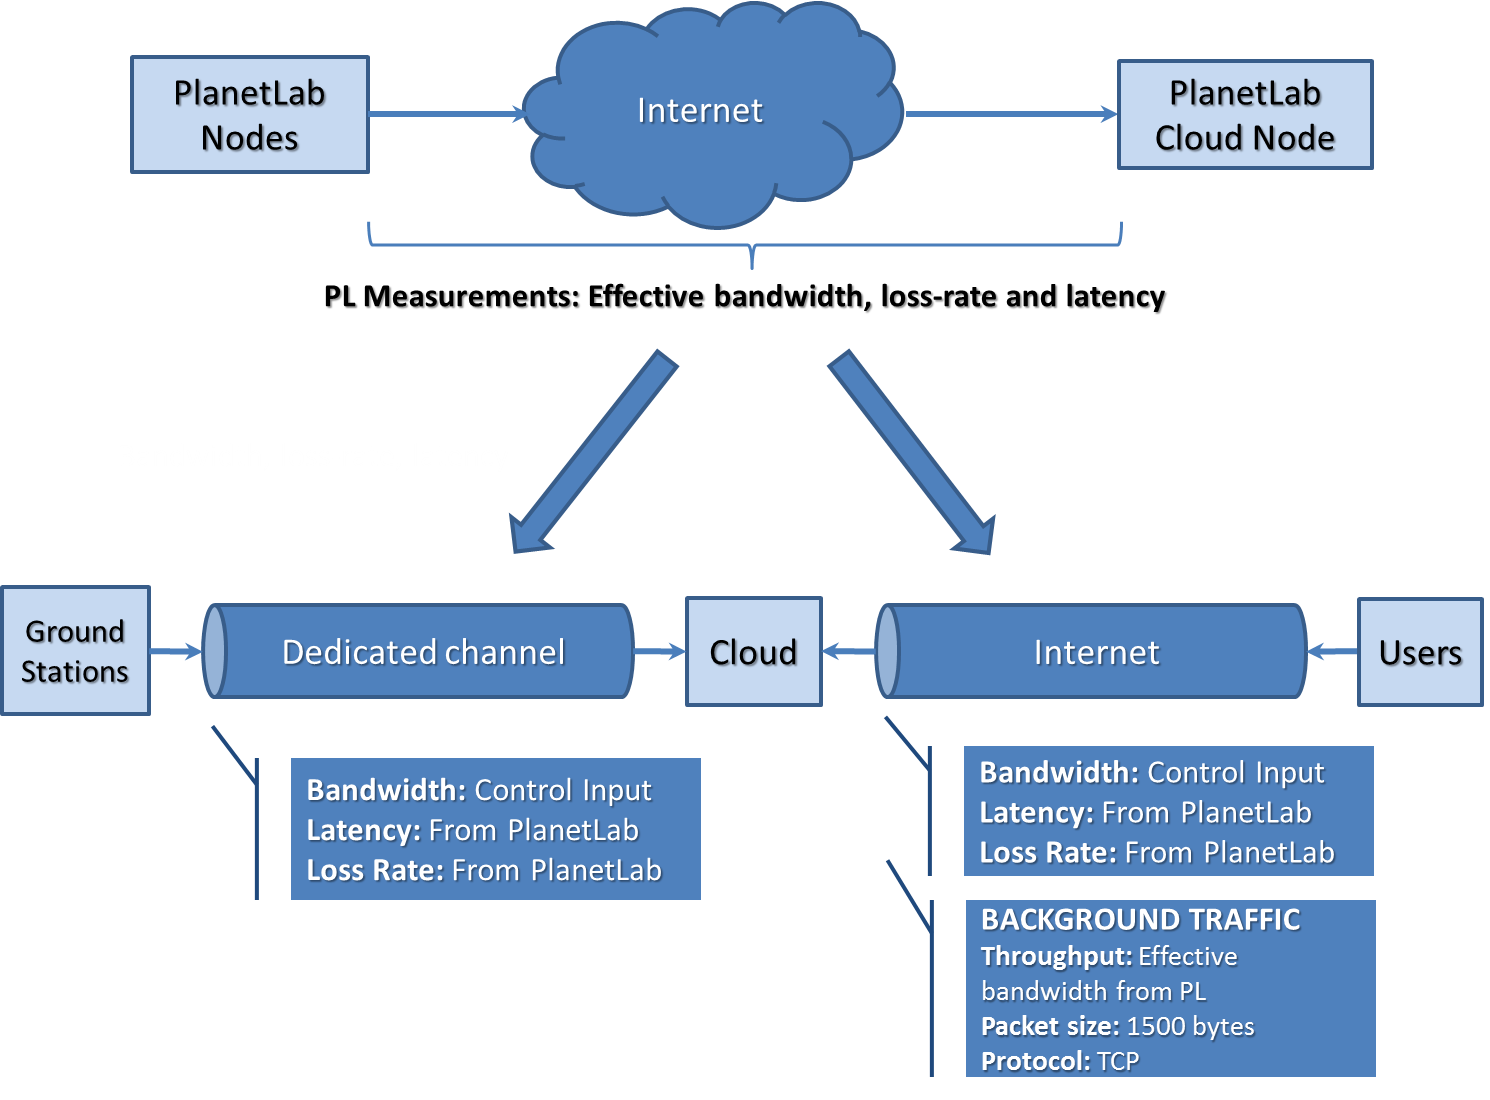
\includegraphics[width=5.22037in,height=3.85406in]{planetlab/modelled-links.png}
\caption{PlanetLab and modelled links equivalences}
\label{fig:ple-modelled-links}
\end{center}
\end{figure}


\subsubsection{System Modeling}

The real system was modeled into three main components: i) a network of ground stations acquiring imagery data from a constellation of optical satellites, ii) a cloud infrastructure that ingests the data from the ground stations, processes it, stores it and distributes it through web services and iii) end users around the world accessing to the web services offered. The system can be divided into two layers:

\begin{enumerate}

\item \emph{Layer 1} is constituted by 12 ground stations connecting with a cloud
  infrastructure. The ground stations and their location are depicted in Table~\ref{table:ple-groundstations-location}. Their locations and footprints are depicted in Figure~\ref{fig:intr-footprints}. The footprints represent the area in which the satellites can establish the communication with the ground stations.

\begin{table}[hp]
  \centering
  {\small
  


\begin{tabular}{p{.2\textwidth}p{.2\textwidth}}
  \tabheadformat
  \tabhead{Ground Station}   &
  \tabhead{Country of GS location}\\
\hline
\textit{Irkutsk}         & Russia \\
\hline
\textit{Puertollano}         & Spain \\
\hline
\textit{Svalbard}         & Norway \\
\hline
\textit{Troll}         & Antarctic \\
\hline
\textit{Chetumal}         & Mexico \\
\hline
\textit{Córdoba}         &  Argentina\\
\hline
\textit{Dubai}         &United Arab Emirates  \\
\hline
\textit{Kourou}         & French Guiana \\
\hline
\textit{Krugersdorp}         &South Africa  \\
\hline
\textit{Malaysia}         &  Malaysia\\
\hline
\textit{Prince Albert}         & Canada \\
\hline
\end{tabular}


% Local variables:
%   coding: utf-8
%   ispell-local-dictionary: "castellano8"
%   TeX-master: "main.tex"
% End:

  }
  \caption{Ground Station Location}
  \label{table:ple-groundstations-location}
\end{table}

% {\centering
% \includegraphics[width=5.37767in,height=2.68448in]{footprints.png} \par}

% {\centering\bfseries
% Figure\ 2\ Footprints of the ground stations.
% \par}

\item \emph{Layer 2} is constituted by the end users accessing the web services
  implemented in cloud. These users are distributed around the world and can be
  governments, emergency services, media and individuals among others.
\end{enumerate}

From the previous layers two networks can be identified: the network between the
ground stations and the cloud and the network between the end users and the
cloud. The system and the interconnections between components are depicted in
Figure~\ref{fig:ple-system-description}. The connections between the ground stations and end users with the
cloud are represented as arrows with different line types to represent that
every connection can have different characteristics and impairments. All the
connections are \ac{TCP}.

\begin{figure}[!h]
\begin{center}
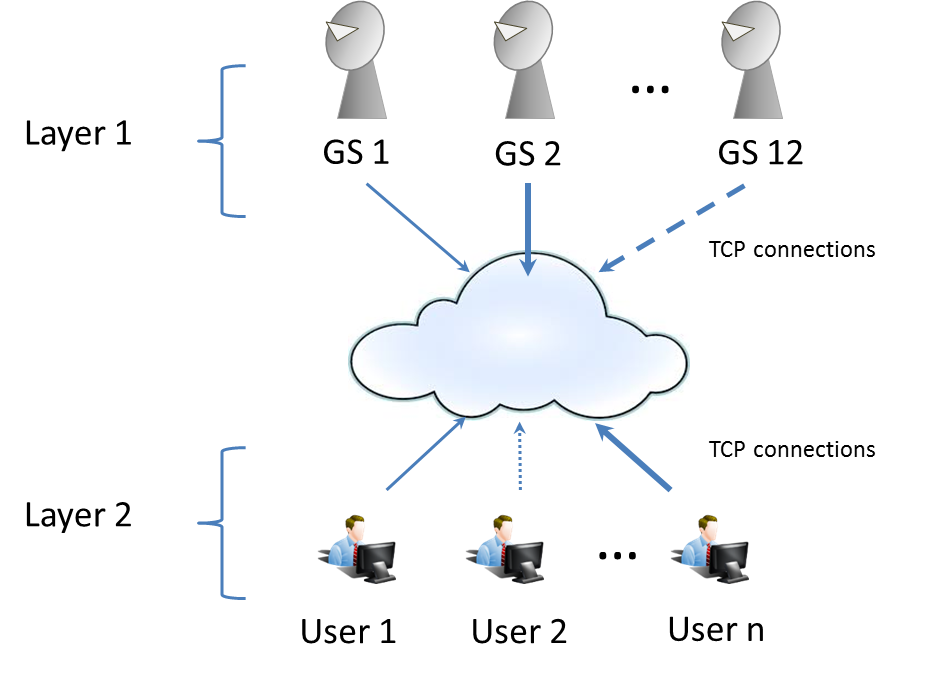
\includegraphics[width=3.35852in,height=2.41008in]{planetlab/system-description.png}

\caption{System description}
\label{fig:ple-system-description}
\end{center}
\end{figure}

The network was defined in function of the following representative impairments: \emph{effective bandwidth, latency and loss rate}. Thus, every link were represented in function of the previous impairments: effective bandwidth, latency, loss rate.
This system was implemented in \vw and \bonfire as depicted in
Figure~\ref{fig:ple-scheme-system}. The experiment in \pl was used to update the
network parameters connecting \vw and \bonfire.

\begin{figure}[!h]
\begin{center}
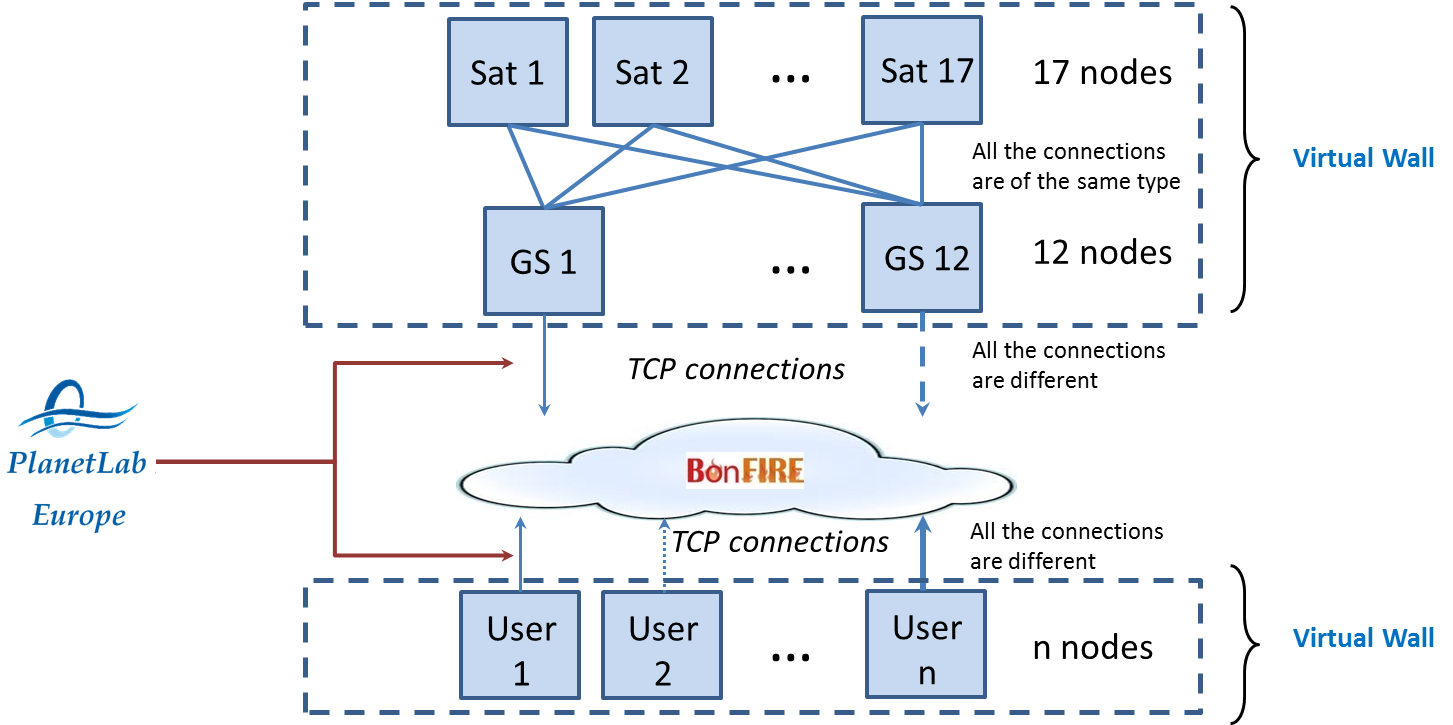
\includegraphics[width=5.48738in,height=2.73818in]{planetlab/schemeSystem.png}
\caption{Scheme of the system implemented in Geo-Cloud}
\label{fig:ple-scheme-system}
\end{center}
\end{figure}


\subsubsection{Network Design}

The model of the ground stations network, the cloud and the end users accessing
the web services provided was simplified to a set of interconnected nodes. The
network was divided into two layers connected by a central node representing the
cloud servers for similarity with the real system:
\begin{itemize}

\item \textbf{Layer 1:} it represents the connections between 12 nodes
  representing the ground stations and a central node representing the cloud
  servers. In \emph{PlanetLab Europe} and \emph{PlanetLab Central}, the nearest nodes to the
  real location of the ground stations were selected. For the central node, a
  node in \emph{INRIA} was chosen, since the \bonfire cloud has servers in the same
  location. This layer then represents the transfer of geodata acquired by the
  constellation of satellites from the ground stations in which the data is
  downloaded to the cloud. The network topology implemented is peer-to-peer,
  i.e. each node representing the ground stations is directly connected with the
  central node. In Table~\ref{tab:ple-tablelayer1-nodes} the \pl selected nodes for layer 1 and for the
  cloud central node are shown. The nodes are numbered in ascending order in
  function of the distance to the central node, i.e. the closest node is the
  number 0 and the furthest the 37.

% \begin{table}[hp]
%   \centering
%   {\small
%   
\begin{tabular}{c c c c c}
\tabheadformat
\tabhead{Ground Station} & \tabhead{Node Location} & \tabhead{Selected Node} & \tabhead{Site} & \tabhead{Node number}\\\hline
             Irkutsk\footnote{These ground stations are located in areas without nodes, the closest node has been selected.} & China & planetlab1.buaa.edu.cn & Beihang University & 24\\
             \hline
             Puertollano & Spain & Planetlab2.dit.upm.es & Universidad Polit\'{e}cnica Madrid  & 5\\
             \hline
             Svalbard & Norway & planetlab1.cs.uit.no & University of Tromso   & 14\\
             \hline
             Troll\footnote{These ground stations are located in areas without nodes, the closest node has been selected.} & New Zealand & planetlab1.cs.otago.ac.nz & University of Otago    & 37\\
             \hline
             Chetumal\footnote{These ground stations are located in areas without nodes, the closest node has been selected.} & USA & Planetlab1.eecs.ucf.edu & University of Central Florida & 22\\
             \hline
             C\'{o}rdoba & Argentina & planet-lab2.itba.edu.ar & Instituto Tecnol\'{o}gico Buenos Aires    & 34\\
             \hline
             Dubai\footnote{These ground stations are located in areas without nodes, the closest node has been selected.} & Israel & planet1.cs.huji.ac.il & The Hebrew University of Jerusalem   & 19\\
             \hline
             Kourou\footnote{These ground stations are located in areas without nodes, the closest node has been selected.} & Brazil & planetlab1.pop-pa.rnp.br & RNP  &26\\
             \hline
             Krugersdorp\footnote{These ground stations are located in areas without nodes, the closest node has been selected.} & Reunion Island (France) & lim-planetlab-1.univ-reunion.fr & Universite de La Reunion    & 28\\
             \hline
             Malaysia & Malaysia & planetlab1.comp.nus.edu.sg & National University of Singapore   & 32\\
             \hline
             Prince Albert & Canada & planetlab-2.usask.ca & University of Saskatchewan    & 21\\
             \hline
             Sidney & Australia & pl1.eng.monash.edu.au & National ICT Australia   & 36\\
             \hline
             Cloud\footnote{Node representing the cloud infrastructure.} & France & ple6.ipv6.lip6.fr & University Pierre et Marie Curie & N/A\\
             \hline
\end{tabular}
%   }
%   \caption{Ground Segment Nodes}
%   \label{tab:ple-tablelayer1-nodes}
% \end{table}


\item \textbf{Layer 2:} it represents the connection between the central node
  representing the cloud servers and the end users. 31 different nodes were
  selected in \emph{PlanetLab Europe} and \emph{PlanetLab} Central in 31 different countries
  around the world. This allows us to have a representative sample of global
  users accessing the web service
s. In this case, the network topology is also peer-to-peer. In Table~\ref{tab:ple-tablelayer2-nodes} the nodes selected for layer 2 are listed. We tried to increase the number of nodes in different countries, but during the execution of the experiment we did not find available PlanetLab nodes in the following countries: Austria, Cyprus, Denmark, Egypt, Ecuador, Iceland, India, Jordan, Mexico, Pakistan, Puerto Rico, Romania, Slovenia, Sri Lanka, Tunisia, Turkey, Venezuela, Uruguay and Taiwan.
\end{itemize}


% \begin{table}[hp]
%   \centering
%   {\small
%   
\begin{tabular}{c c c c c c }
\tabheadformat
\tabhead{Country} & \tabhead{Selected Node} & \tabhead{Number} &\tabhead{Country} & \tabhead{Selected Node} &\tabhead{Number}\\\hline
       Argentina  & planet-lab2.uba.ar                 & 35  &   Japan & planet1.pnl.nitech.ac.jp                &  31 \\\hline
       Australia & pl1.eng.monash.edu.au               & 36  &   Korea, Republic of & netapp7.cs.kookmin.ac.kr   &  27 \\\hline
       Belgium & rochefort.infonet.fundp.ac.be         & 2  &   The Netherlands & planetlab1.cs.vu.nl          & 4   \\\hline
       Brazil & planetlab1.pop-pa.rnp.br               & 26  &   New Zealand & planetlab1.cs.otago.ac.nz         &  37 \\\hline
       Canada & planetlab-2.usask.ca                   & 21  &   Norway & planetlab1.cs.uit.no                   &  14 \\\hline
       China & planetlab1.cqupt.edu.cn                 & 25  &   Poland & ple2.dmcs.p.lodz.pl                    &  13 \\\hline
       Czech Republic & planetlab1.cesnet.cz           & 8  &   Portugal & planet1.servers.ua.pt                & 11  \\\hline
       Finland & planetlab-1.research.netlab.hut.fi    & 17  &   Russian Federation & plab1.cs.msu.ru            & 20  \\\hline
       France & inriarennes2.irisa.fr                  & 0  &   Singapore & planetlab1.comp.nus.edu.sg          &   33\\\hline
       Germany & planetlab02.tkn.tu-berlin.de          & 6  &   Spain & dplanet2.uoc.edu                        &  3 \\\hline
       Greece & planetlab1.ionio.gr                    & 15  &   Sweden & planetlab2.s3.kth.se                   & 16  \\\hline
       Hong Kong & planetlab1.ie.cuhk.edu.hk           & 30  &   Switzerland & planetlab2.unineuchatel.ch        &  1 \\\hline
       Hungary & planet2.elte.hu                       & 12  &   Thailand & ple2.ait.ac.th                       & 29  \\\hline
       Ireland & planetlab-node-01.ucd.ie              & 10 &   United Kingdom & planetlab-2.imperial.ac.uk     &  9 \\\hline
       Israel & planetlab2.tau.ac.il                   & 18  &   United States & planetlab-04.cs.princeton.edu   & 23  \\\hline
       Italy & planet-lab-node1.netgroup.uniroma2.it   & 7  &           &    &\\\hline
\end{tabular}

%   }
%   \caption{User Nodes}
%   \label{tab:ple-tablelayer2-nodes}
% \end{table}


Figure~\ref{fig:ple-network-scheme} shows a scheme representing the network created in \pl. The
connections between the nodes are \emph{TCP}.

\begin{figure}[!h]
\begin{center}
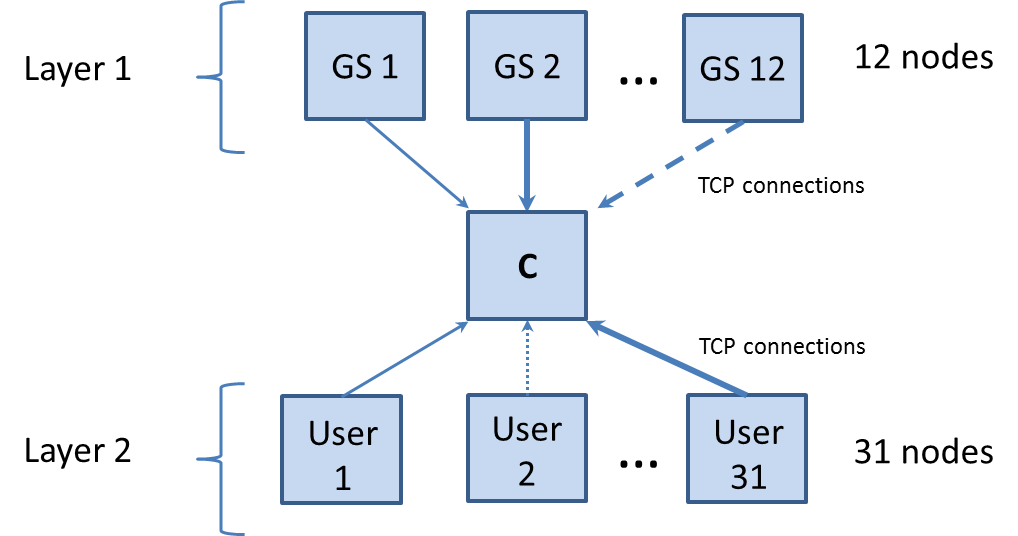
\includegraphics[width=4.01423in,height=2.11349in]{planetlab/network-scheme.png}

\caption{PlanetLab Network Scheme}
\label{fig:ple-network-scheme}
\end{center}
\end{figure}

\subsubsection{Experiment Design and Execution}

The experiment was designed to measure the impairments of the network. Those
impairments are required parameters in \vw to deploy a topology network in such
a testbed. Then, the latency, loss-rate and effective bandwidth were
measured. The deployment of the experiment was done with \nepi, in which
\emph{Iperf} and \emph{Ping} were implemented to measure the impairments. The
experiment consists of establishing communications between any node in layer 1
or layer 2 with the central node and measuring the previously described
impairments. 21600 trials were performed during 6 hours of the experiment execution in steps of one second for each pair of nodes, i.e. a node from layer 1 or 2 and the central node.

The software developed to measure the impairments is constituted of 6 scripts:
\begin{itemize}
\item Script to measure the effective bandwidth in the ground stations nodes: “bandwidthGS.py”.
\item Script to measure the effective bandwidth in the end users nodes: “bandwidthEndUser.py”
\item Script to measure the latency in the ground stations nodes: “latencyGS.py”.
\item Script to measure the latency  in the end users nodes: “latencyEndUser.py”
\item Script to measure the loss rate in the ground stations nodes: “lossRateGS.py”
\item Script to measure the loss rate in the end users nodes:
  “lossRateEndUser.py”

\end{itemize}

The pair of scripts that measure the same impairment are differentiated one from each other in the provisioning of the nodes. Those nodes representing the ground stations are manually selected, while the end users nodes are automatically provisioned by \nepi by indicating the country name as parameter. This parameter allows \nepi to select an available node in that country.

The previous six scripts were individually executed in a local host and they started their workflow.

\paragraph{The bandwidthGS.py script}~\\

The \emph{bandwidthGS.py}  script measures the effective bandwidth in the ground
stations nodes. When it is executed it carries out the next tasks:
\begin{enumerate}
\item Provisioning of the nodes that were manually selected.
\item Creation of the commands to be uploaded:
\begin{itemize}
\item In the cloud node:

\emph{timeout \%dm iperf -s -f m -i 1 -p \%d} \\
\emph{Timeout} is a command that executes a program during a specified time \%dm in
minutes. For this experiment $dm$ was chosen to be 6 hours.
\begin{itemize}
\item s indicates that \emph{Iperf} is executed in server mode
\item f m indicates the format to report the received data. In this case in $Mb$.
\item i 1 Periodic reports every 1 second
\item p \%d indicates the port to listen. In this case 20004.
\end{itemize}

\item In the ground station nodes:

\emph{iperf  -i 1 -f m -c \%s -t \%d -p \%d  -y c > node\%d.out}\\
\begin{itemize}
\item i 1 Periodic reports every 1 second.
\item f m indicates the format to report the received data. In this case in Mb.
\item c \%s indicates the server to establish the communication with.
\item t indicates the data transmission time. In this case 3600 seconds.
\item p \%d indicates the port to listen. In this case 20004.
\item y c> node\%d.out indicates that the report format is \ac{CSV}. The output file
  is node\%d.out, where \%d indicates the number of the node tested.
\end{itemize}
\end{itemize}

By default \emph{Iperf} is executed in \ac{TCP} mode.

\item Uploads the commands to the nodes
\item Executes the command in cloud
\item Executes the command in the rest of nodes
\item During the execution of the commands the data is collected
\item Finishes the execution of the commands
\item The data collected is retrieved
\item The resources are released.
\end{enumerate}

The flow diagram of the effective bandwidth measurements in the ground station nodes is depicted in Figure~\ref{fig:ple-workflow-ground-bandwidth}.

\paragraph{The bandwidthEndUser.py script}~\\

The \emph{bandwidthEndUser.py} script measures the effective bandwidth in the
end users nodes. When it is executed it carries out the next tasks:
\begin{enumerate}
\item Automatic provisioning of the nodes.
\item Tasks 2 to 9 of the \emph{bandwidthGS.py} script.
\end{enumerate}

The flow diagram of the effective bandwidth measurements in the end users nodes is depicted in Figure~\ref{fig:ple-workflow-enduser-bandwidth}.

\paragraph{The lossRateGS.py script}~\\

The \emph{lossRateGS.py}  script measures the loss rate in the ground stations
nodes. When it is executed it carries out the next tasks:

\begin{enumerate}
\item Provisioning of the nodes that were manually selected.
\item Creation of the commands to be uploaded:
\begin{itemize}
\item In the cloud node:

\emph{timeout \%dm iperf -s -f m -i 1 -p \%d -u} \\
\emph{Timeout} is a command that executes a program during a specified time \%dm in
minutes. For this experiment dm was chosen to be 6 hours.%65 minutos
\begin{itemize}
\item s indicates that \emph{Iperf} is executed in server mode
\item f m indicates the format to report the received data. In this case in $Mb$.
\item i 1 Periodic reports every 1 second
\item p \%d indicates the port to listen. In this case 20004.
\item u indicates that the \emph{Iperf} software is executed in \emph{UDP} mode.
\end{itemize}

\item In the ground station nodes:

\emph{iperf  -i 1 -f m -c \%s -t \%d -p \%d  -y c > node\%d.out}\\
\begin{itemize}
\item i 1 Periodic reports every 1 second.
\item f m indicates the format to report the received data. In this case in \emph{Mb}.
\item c \%s indicates the server to establish the communication with.
\item t indicates the data transmission time. In this case 3600 seconds.
\item p \%d indicates the port to listen. In this case 20004.
\item y c> node\%d.out indicates that the report format is \ac{CSV}. The output file
  is node\%d.out, where \%d indicates the number of the node tested.
\item u indicates that the \emph{Iperf} software is executed in \emph{UDP} mode.
\end{itemize}
\end{itemize}

By default \emph{Iperf} is executed in \ac{TCP} mode.

\item Uploads the commands to the nodes
\item Executes the command in cloud
\item Executes the command in the rest of nodes
\item During the execution of the commands the data is collected
\item Finishes the execution of the commands
\item The data collected is retrieved
\item The resources are released.
\end{enumerate}

The flow diagram of the loss rate measurements in the ground station nodes is
depicted in Figure~\ref{fig:ple-workflow-ground-bandwidth}.

\paragraph{The lossRateEndUser.py script}~\\

The \emph{lossRateEndUser.py} script measures the loss rate in the end users
nodes. When it is executed it carries out the next tasks:
\begin{enumerate}
\item Automatic provisioning of the nodes.
\item Tasks 2 to 9 of the \emph{lossRateGS.py} script.
\end{enumerate}
The flow diagram of the loss-rate measurements in the end users nodes is
depicted in Figure~\ref{fig:ple-workflow-enduser-bandwidth}.

\paragraph{The latencyGS.py script}~\\

The \emph{latencyGS.py}  script measures the latency  in the ground stations
nodes. When it is executed it carries out the next tasks:
\begin{enumerate}

\item Provisioning of the nodes that were manually selected.
\item Creation of the commands to be uploaded:

\emph{ping \%s -w \%d}
\begin{itemize}
\item \%s indicates the host to do ping
\item w \%d indicates the time of the ping execution.
\end{itemize}
\item Uploads the commands to the nodes
\item Executes the command in cloud
\item Executes the command in the rest of nodes
\item During the execution of the commands the data is collected
\item Finishes the execution of the commands
\item The data collected is retrieved
\item The resources are released.
\end{enumerate}

The flow diagram of the latency measurements in the ground station nodes is depicted in Figure~\ref{fig:ple-workflow-latency-ground}.

\paragraph{The latencyEndUser.py script}~\\

The \emph{latencyEndUser.py}  script measures the latency in the end users
nodes. When it is executed it carries out the next tasks:
\begin{enumerate}
\item Automatic provisioning of the nodes.
\item Tasks 2 to 9 of the \emph{latencyGS.py} script.
\end{enumerate}

The flow diagram of the latency measurements in the end users nodes is depicted
in Figure~\ref{fig:ple-workflow-latency-user}.

\begin{figure*}
\begin{center}
\subfloat[Flow diagram of the \emph{bandwidthEndUser.py} and \emph{lossRateEndUser.py} scripts]{ 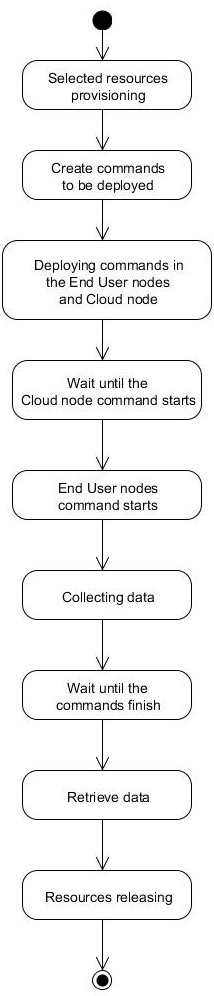
\includegraphics[width=0.2\textwidth]{planetlab/PLClient.jpg}
\label{fig:ple-workflow-enduser-bandwidth}}
\hspace{0.03\textwidth}
\subfloat[Flow diagram of the \emph{bandwidthGS.py} and \emph{lossRateGS.py} scripts]{ 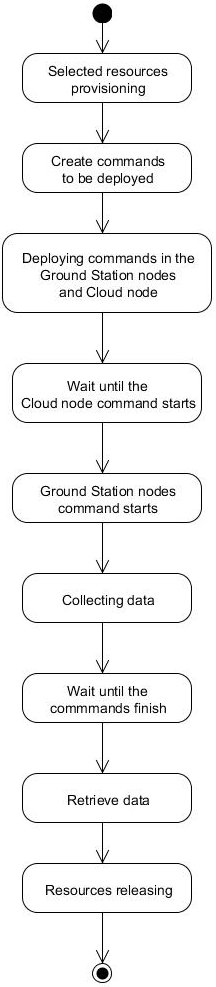
\includegraphics[width=0.2\textwidth]{planetlab/PLGS.jpg}
\label{fig:ple-workflow-ground-bandwidth}}
\hspace{0.03\textwidth}
\subfloat[Flow diagram of the \emph{latencyGS.py} script]{ 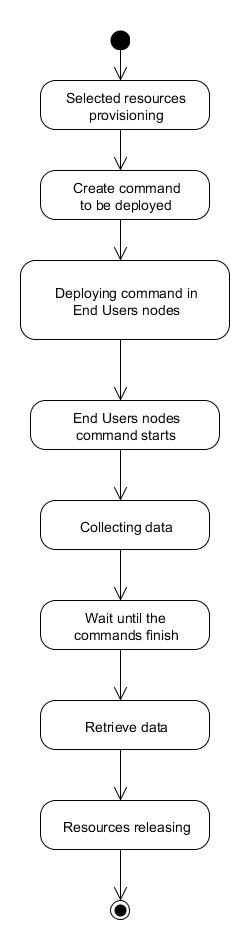
\includegraphics[width=0.2\textwidth]{planetlab/PLPINGClients.jpg}
\label{fig:ple-workflow-latency-user}}
\hspace{0.03\textwidth}
\subfloat[Flow diagram of the \emph{latencyEndUser.py} script]{ 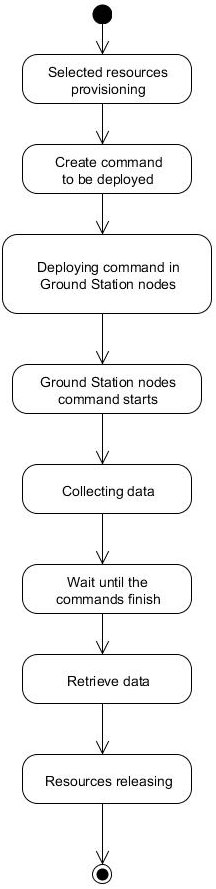
\includegraphics[width=0.2\textwidth]{planetlab/PLPINGGS.jpg}
\label{fig:ple-workflow-latency-ground}}
\end{center}
\end{figure*}



\section{PlanetLab Experiment Results}
\label{sec:pl-res}
During the execution of the \pl experiment (see Section~\ref{sec:planetlab}) 21600 communications were established between every node representing ground stations and users and the central node representing the cloud. The bandwidth, latency and loss rate were measured.
In Figure~\ref{fig:Bandwidth_gs_hist} the 21600 samples acquired in the communication between the node 22 and the central node during 6 hours of continuous execution are represented in a normalized histogram. The data accurately fits to a gaussian distribution with mean $3.28~Mbps$ and standard deviation $0.446~Mbps$. In Figure~\ref{fig:Latency_gs_hist} a normalized histogram of the measured latency is represented. It was fitted with a gaussian distribution with mean $154.210~ms$ and standard deviation $1.314~ms$. The loss rate between this node and the central node was obtained to be $0.0096$\%~\cite{Gonzalez2014}.
\begin{figure*}
\begin{center}
  \subfloat[Bandwidth of the node representing Chetumal ground station]{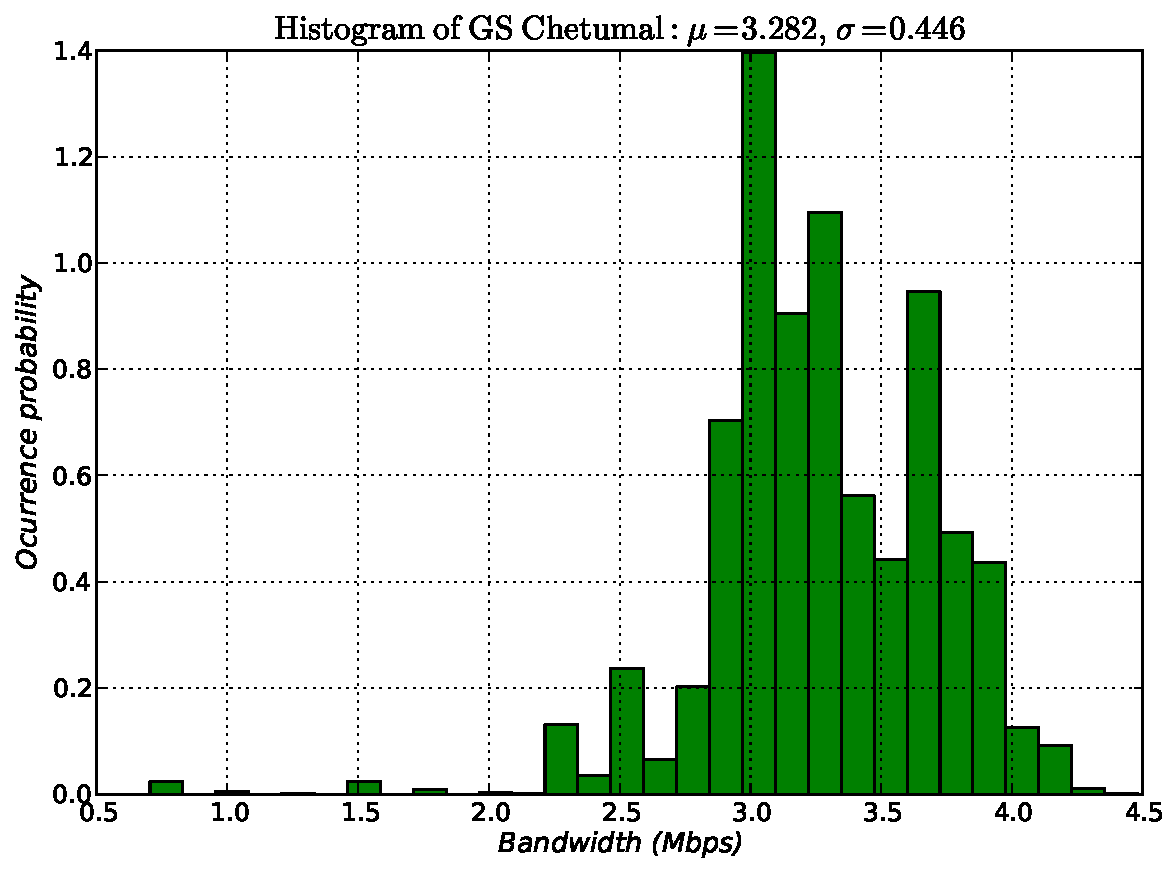
\includegraphics[scale=0.35]{resultsPL/IndividuallyGSHistChetumal.pdf}
 \label{fig:Bandwidth_gs_hist}}
\hspace{0.01\textwidth}
\subfloat[Latency of the node representing Chetumal ground
station]{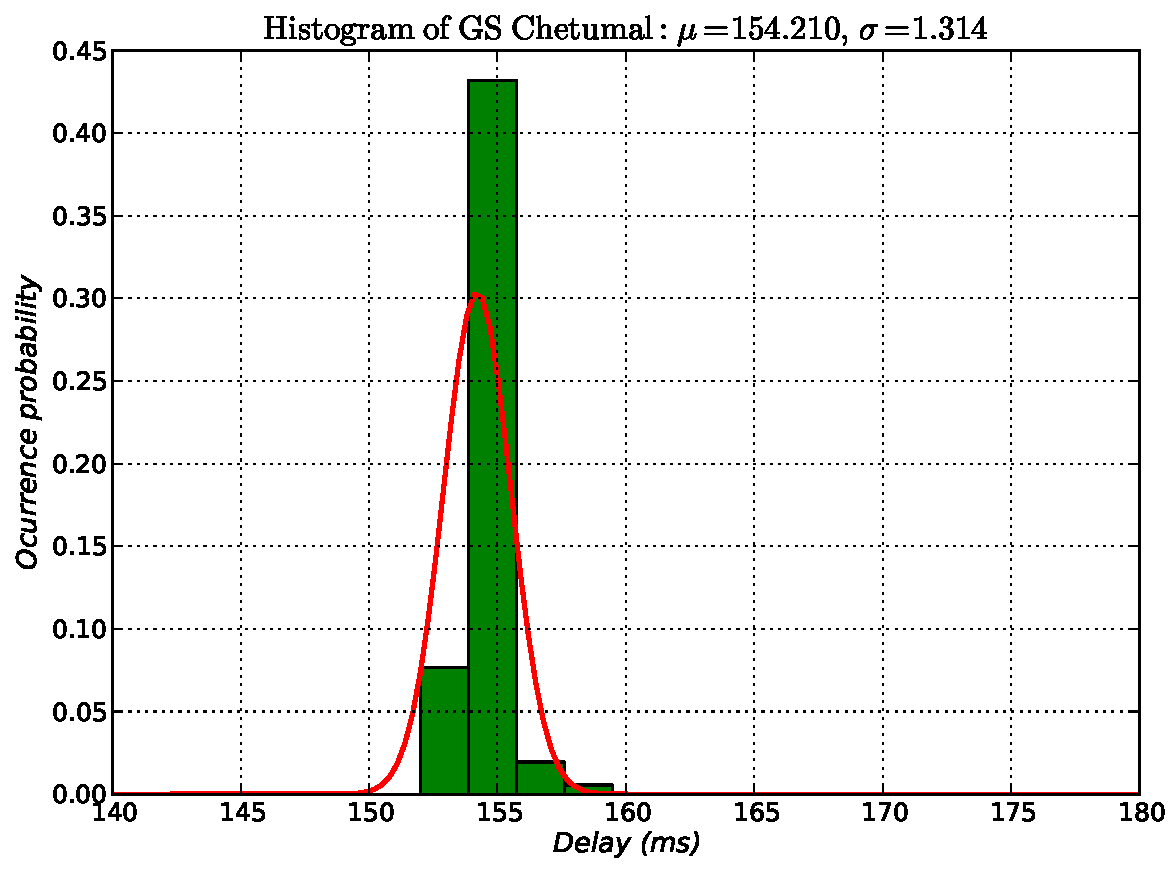
\includegraphics[scale=0.35]{resultsPL/DelayHistGSChetumal.pdf}
 \label{fig:Latency_gs_hist}}
\end{center}
\end{figure*}



The previous procedure was followed for the rest of the nodes. In
Figure~\ref{fig:bandwidth-plot} the mean and the standard deviation for each
node are depicted respectively. It can be observed that in general, the
bandwidth decreases when the distance between nodes increases. However the node
5 in Madrid presents a higher dispersion in the bandwidth value with respect to
the rest of nodes. It has a bandwidth of $15.2~Mbps$. The measurements were
fitted with different functions by using the least squares optimization
method. Exponential, polynomial, logarithm and hyperbolic functions were used to
fit the samples. For each fitted function the $R^2$ coefficient of
determination, which varies between 0 and 1, and indicates how well the
statistical distribution is fitted. The highest the value of the $R^2$, the
better the fitting. The following results were obtained: for exponential
function: $Bandwidth=4.655e^{-10^{-4}x}$,$R^2=0.5454$; for polynomial function
$Bandwidth=-3\cdot10^{-4}x+4.9444$, $R^2=0.3628$ and for logarithm function $Bandwidth=-1.519Ln(x)+15.325$, $R^2=0.4539$, where $x$ is the distance between any node and the central node in $km$. The bandwidth was obtained in $Mbps$. However, the hyperbolic function was the one that best fitted the distribution:
\begin{equation}\label{eq:bandwidth_fitting}
Bandwidth=184.91x^{-0.547};~R^2=0.582
\end{equation}

\begin{center}
\begin{figure}[h]
  \centering
  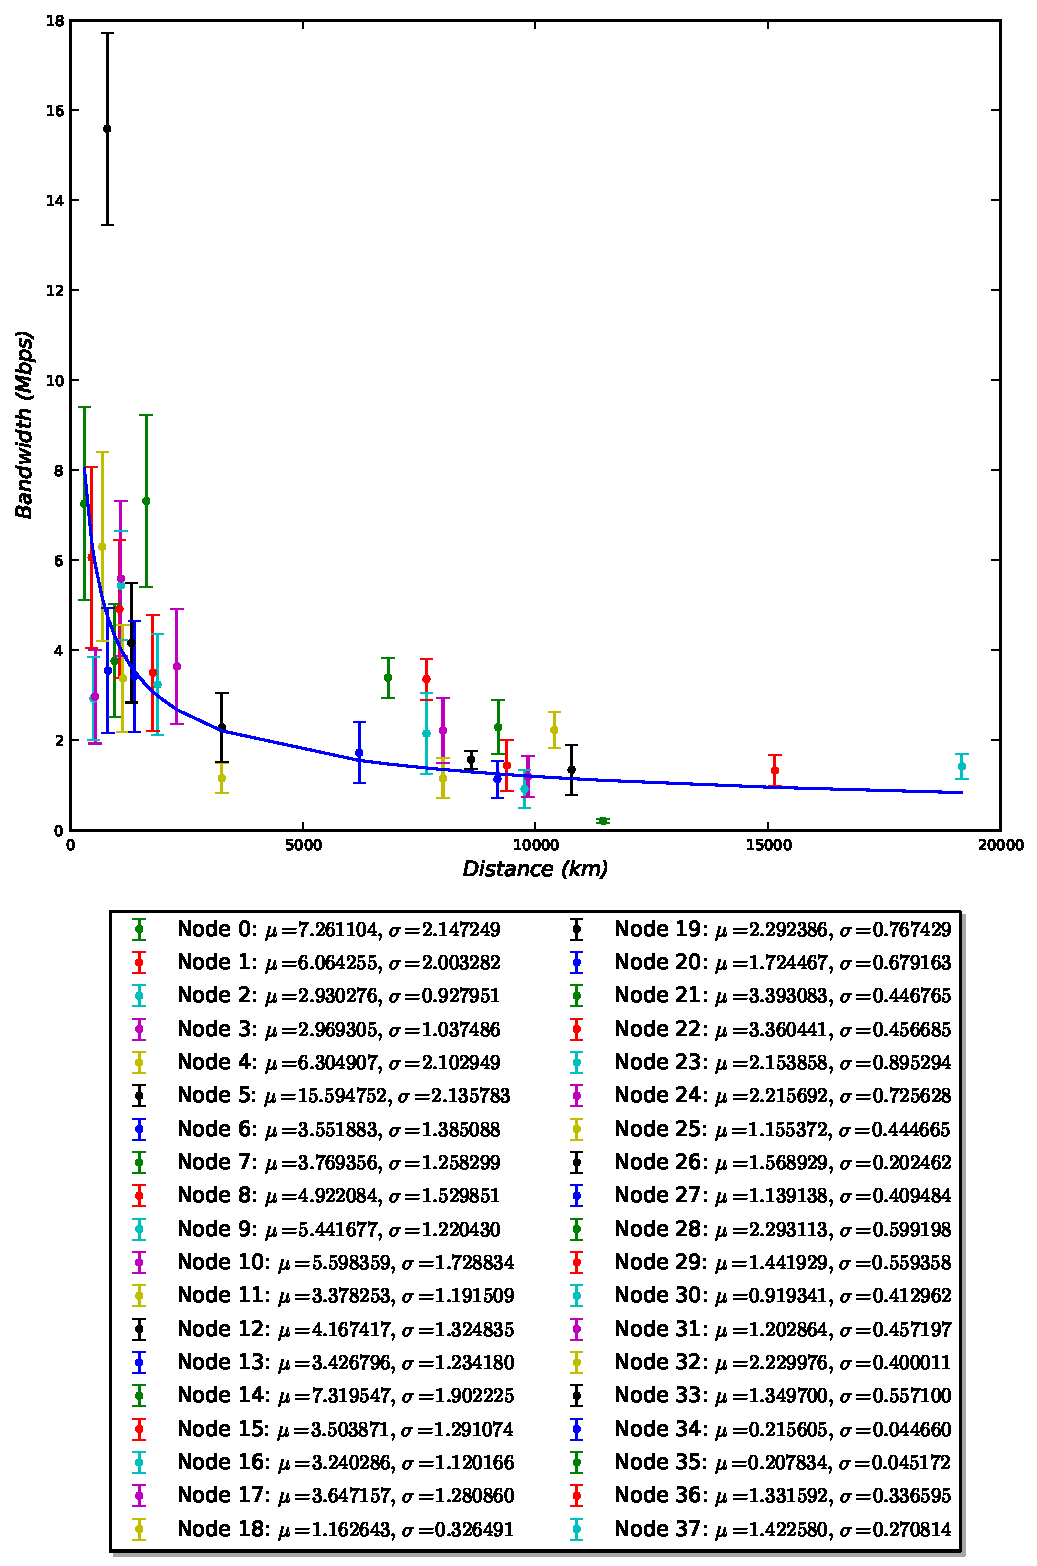
\includegraphics[scale=0.7]{resultsPL/bandwidthall.pdf}\\
  \caption{Bandwidth of all nodes} \label{fig:bandwidth-plot}
\end{figure}
\end{center}

Figure~\ref{fig:delay-plot} shows the mean and standard
deviation of the latency measured in all the nodes connecting the central node
in France. In this case the fitting used was a linear function. It accurately fitted the data distribution. The equation that approximated the data is the following:
\begin{equation}\label{eq:latency_fitting}
Latency=0.0228x+17.88;~R^2=0.8927
\end{equation}
The latency is obtained in $ms$ when the distance $x$ is introduced in $km$.


\begin{center}
\begin{figure}[h]
  \centering
  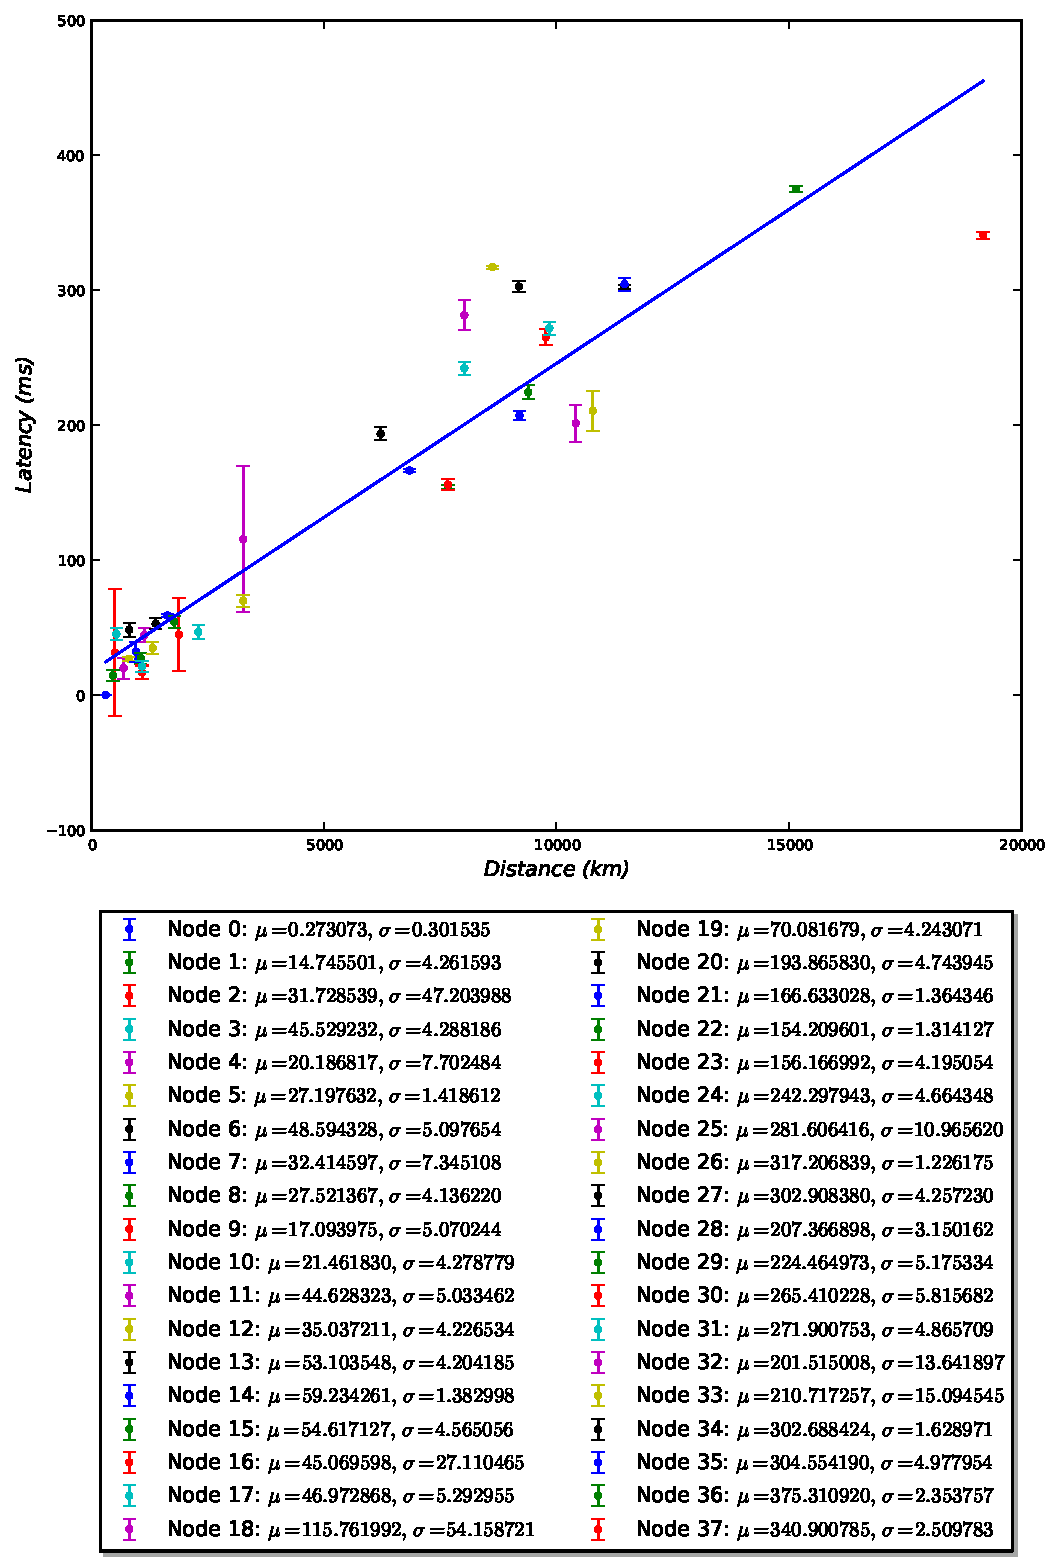
\includegraphics[scale=0.7]{resultsPL/DelayNodes.pdf}\\
  \caption{Latency of all nodes} \label{fig:delay-plot}
\end{figure}
\end{center}

Figure~\ref{fig:loss-rate-plot} shows the loss rate between any node and the central node during the whole execution of the experiment. In most of the communications the loss rate was under 0.2\%. Two cases are remarkable: on the one hand, between the node 20 in Russia and the central node 0\% of loss rate was measured, which means that no packets were lost; on the other hand, between Greece (node 16) and the central node, a loss rate of 15.68\% was measured, maybe because of interruptions in the network, overload of the server in Greece or routed network fails. The mean of the loss rates between all the communications was 0.053\% with a standard deviation of 0.097\% without considering the node in Greece in the calculations.

Table~\ref{anex:nodes-pl-results} summarizes the obtained measures. Column 5 and 6 show the mean and
the standard deviation of the bandwidth measured in all the nodes connecting the
central node in France. Column 7 and 8 also depict the mean and standard
deviation of the latency in the nodes. Finally, column 9 represents the measured
loss-rate between any node and the central node during the experiment.




\begin{center}
\begin{figure}[h]
  \centering
  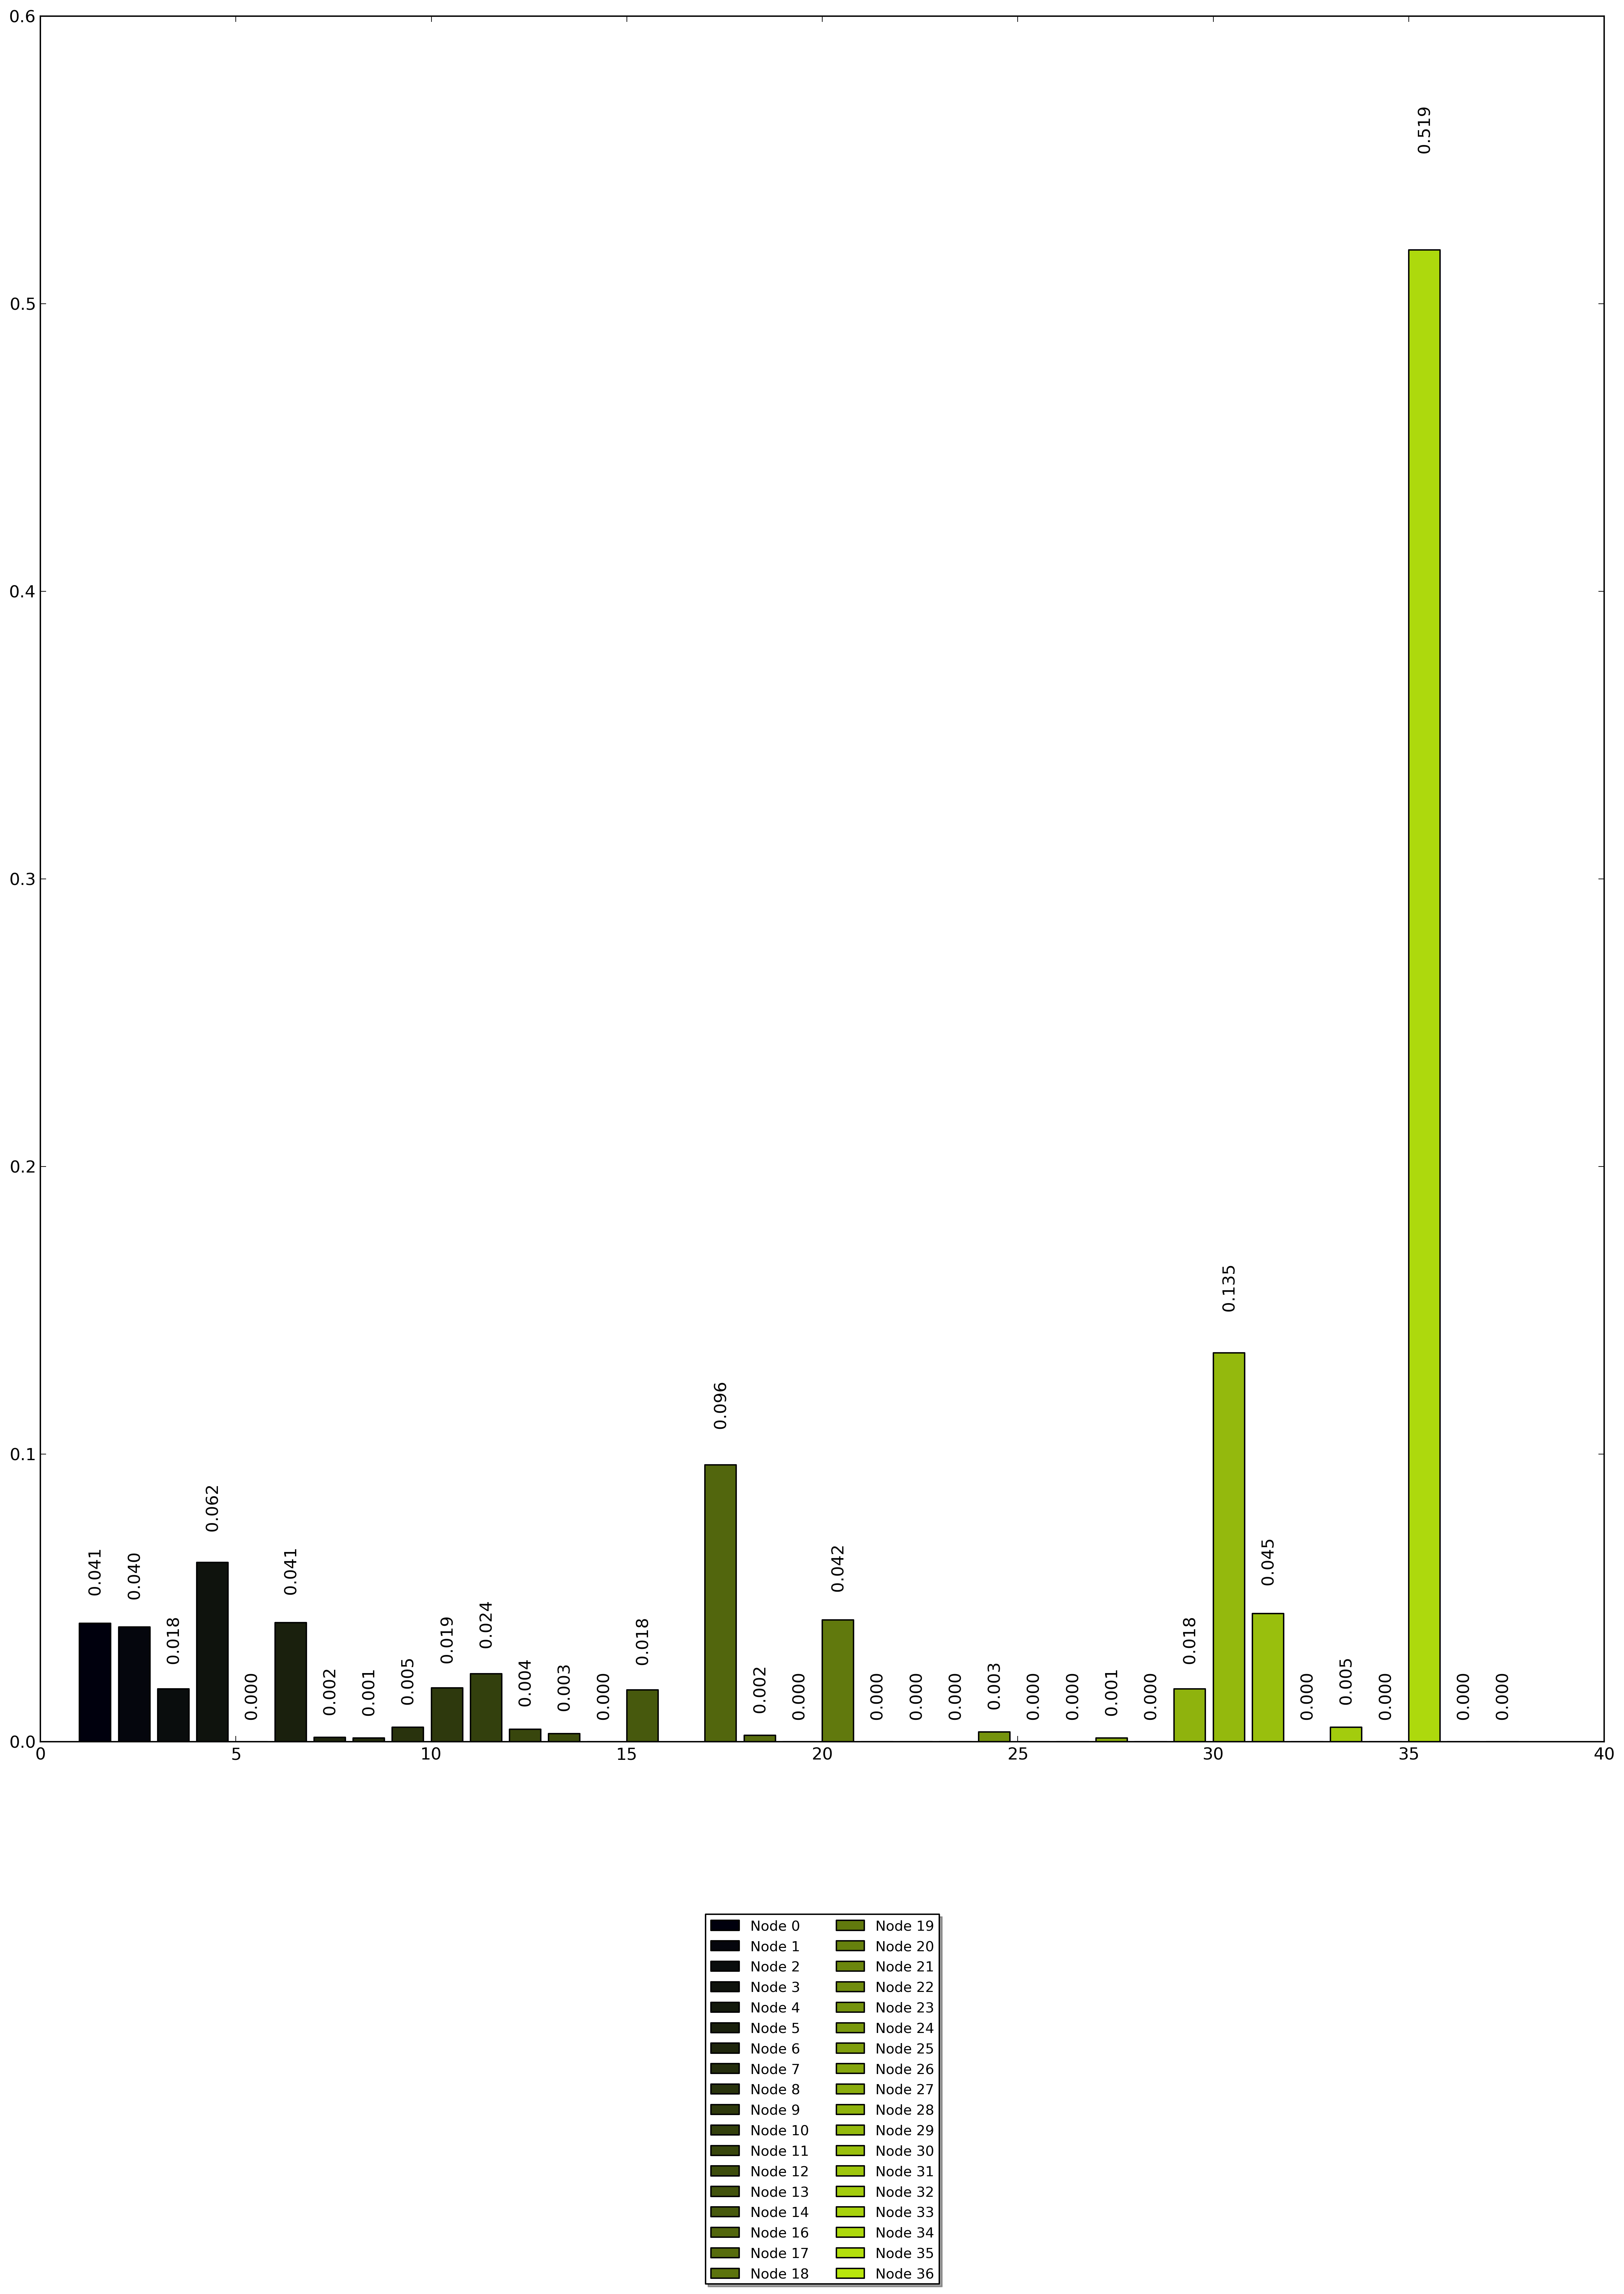
\includegraphics[scale=0.7]{resultsPL/Loss-rateALL.png}\\
  \caption{Bandwidth of all nodes.} \label{fig:loss-rate-plot}
\end{figure}
\end{center}



\section{GEO-Cloud Graphical User Interface}

In this section, the \ac{GUI} developed for managing the execution of the defined
scenarios in GEO-Cloud experiment is exposed. First, the architecture is
explained. The components such as \emph{ExperimentController}, \emph{Video
  Component}, \emph{Log Component}, \emph{About Component} and \emph{WorkLoad component} are described. Finally, the workflow is explained.

\subsection{Architecture}

The graphical user interface of GEO-Cloud experiment is composed by the following components:

\begin{itemize}

\item \emph{Experiment Controller}: it manages the \sss turning on or shutting it down.
\item \emph{Video Component}: it shows a video demonstration of the satellite constellation acquiring images at same time that the satellites in \vw.
\item \emph{About Component}: it shows the \emph{About} window where the acknowledments are shown.
\item \emph{Log Component}: it prints the logs which receives from satellites and ground stations.
\item \emph{Workload component}: it plots the workload of the Orchestrator and Processing chain machine.

\end{itemize}

The Figure~\ref{} shows the architecture where the relations between the components are pictured.

%esquema architectur

\subsubsection{Experiment Controller}

This component connects with the \sss for managing it execution. Basically, this component is constituted by the following classes: the ExperimentController class, VWConnection class and JFedParser class. This classes controls, connects and parsers the execution of the \sss, obtains the connections with \sss nodes and process a configuration file in order to obtain the \sss nodes hostnames, respectively.

The ExperimentController sequentially follows the next steps during the execution:
\begin{itemize}
\item First, the JFedParser is created and it parsers the contain of the file namely ``jfed.out'' located 

\end{itemize}

\subsubsection{Video Component}

This 

\subsection{About Component}

\subsection{Log Component}

\subsection{Workload Component}








% Local Variables:
%   coding: utf-8
%   fill-column: 90
%   mode: flyspell
%   ispell-local-dictionary: "american"
%   mode: latex
%   TeX-master: "main"
% End:

